\documentclass[12pt,a4paper,twocolumn,fleqn]{article}
\usepackage{graphicx}
\usepackage[colorlinks=true,linkcolor=black,anchorcolor=black,citecolor=black,filecolor=black,menucolor=black,runcolor=black,urlcolor=black]{hyperref}
\usepackage{chngcntr}
\counterwithin{figure}{section}
\usepackage[a4paper,top=20mm, bottom=30mm, left=18mm, right=18mm]{geometry}
\usepackage{fancyhdr}
\usepackage{tikz}
\usetikzlibrary{calc}
\usepackage{eso-pic}
\usepackage[shortlabels]{enumitem}
\usepackage{hyperref}
\usepackage{lastpage}
\usepackage{listings}
\usepackage[]{algorithm2e}
\usepackage{color}
\usepackage{fancybox}
\usepackage{lineno}
\usepackage{xtab,booktabs}
\usepackage{setspace}
\usepackage{amsmath}
\usepackage{xcolor}
\usepackage[compact]{titlesec}
\titleformat{\section}[block]{\color{black}\Large\bfseries\filcenter}{}{1em}{}
\titlespacing{\section}{0pt}{*0}{*0}
\titlespacing{\subsection}{0pt}{*0}{*0}
\titlespacing{\subsubsection}{0pt}{*0}{*0}
\setlength\columnsep{25pt}
\makeatletter
\g@addto@macro{\normalsize}{%
\setlength{\abovedisplayskip}{0pt}
\setlength{\abovedisplayshortskip}{0pt}
\setlength{\belowdisplayskip}{0pt}
\setlength{\belowdisplayshortskip}{0pt}}
\makeatother
\makeatletter
\renewenvironment{abstract}{%
    \if@twocolumn
      \section*{\abstractname}%
    \else %% <- here I've removed \small
      \begin{center}%
        {\bfseries \Large\abstractname\vspace{\z@}}%  %% <- here I've added \Large
      \end{center}%
      \quotation
    \fi}
    {\if@twocolumn\else\endquotation\fi}
\makeatother
\makeatletter
\let\latexl@section\l@section
\def\l@section#1#2{\begingroup\let\numberline\@gobble\latexl@section{#1}{#2}\endgroup}
\makeatother
\mathindent=0.0pt
\usepackage{float}
\renewcommand{\baselinestretch}{1.5}
\AddToShipoutPictureBG*{%
\begin{tikzpicture}[overlay,remember picture]
\draw[line width=4pt]
    ($ (current page.north west) + (1.3cm,-1.5cm) $)
    rectangle
    ($ (current page.south east) + (-1.3cm,1.5cm) $);
\draw[line width=1.5pt]
    ($ (current page.north west) + (1.5cm,-1.7cm) $)
    rectangle
    ($ (current page.south east) + (-1.5cm,1.7cm) $);
\end{tikzpicture}
}
\begin{document}
\pagestyle{empty}
\onecolumn
\begin{center}
\text{A Project Report On} \\
\smallskip
\textcolor{red}{\LARGE{Foodereum: A Blockchain-based Authenticated Solution for Food Supply Chain}} \\
\large{Submitted in partial fulfillment of the requirement for the $8^{th}$ semester} \\
\large{\textbf{Bachelor of Engineering}} \\
\large{in} \\
\large{Computer Science and Engineering} \\
\textcolor{blue}{\LARGE{DAYANANDA SAGAR COLLEGE OF ENGINEERING}} \\
\footnotesize{(An Autonomous Institute affiliated to VTU, Belagavi, Approved by AICTE \& ISO 9001:2008 Certified)} \\
\footnotesize{Accredited by National Assessment \& Accreditation Council (NAAC) with ‘A’ grade}  \\
\footnotesize{Shavige Malleshwara Hills, Kumaraswamy Layout, Bengaluru-560078} \\

\includegraphics[scale=0.4]{media/DSCE-min.png} \\
\textit{Submitted By} \\
\textbf{Gautam Kumar \space 1DS18CS710} \\
\textbf{Rithvik K Bhat \space 1DS18CS732} \\
\textbf{Vignesh K \space 1DS18CS744} \\ 
\textbf{[8th Semester,B.E.(CSE)]} \\ 
\hfill
\\
\textit{Under the guidance of} \\
\textbf{Dr. Nagaraja J } \\
\text{Associate Professor, CSE , DSCE} \\
\Large{\textbf{2021 - 2022}} \\
\textcolor{blue}{\Large{Department of Computer Science and Engineering}} \\
\textcolor{blue}{\Large{DAYANANDA SAGAR COLLEGE OF ENGINEERING}} \\
\textcolor{blue}{\Large{Bangalore - 560078}} \\
\end{center}
\newpage
  \pagestyle{fancy}
  \fancyhf{}
  \thispagestyle{empty}
\AddToShipoutPictureBG*{%
\begin{tikzpicture}[overlay,remember picture]
\draw[line width=4pt]
    ($ (current page.north west) + (1.3cm,-1.5cm) $)
    rectangle
    ($ (current page.south east) + (-1.3cm,1.5cm) $);
\draw[line width=1.5pt]
    ($ (current page.north west) + (1.5cm,-1.7cm) $)
    rectangle
    ($ (current page.south east) + (-1.5cm,1.7cm) $);
\end{tikzpicture}
}
\begin{center}
\textcolor{red}{\LARGE{VISVESVARAYA TECHNOLOGICAL UNIVERSITY}} \\
\textcolor{red}{\LARGE{Dayananda Sagar College of Engineering}} \\
\footnotesize{(An Autonomous Institute affiliated to VTU, Belagavi, Approved by AICTE \& ISO 9001:2008 Certified)} \\
\footnotesize{Accredited by National Assessment \& Accreditation Council (NAAC) with ‘A’ grade}  \\
\footnotesize{Shavige Malleshwara Hills, Kumaraswamy Layout, Bengaluru-560078} \\
\begin{flushleft}
\textcolor{blue}{\LARGE{\textbf{Department of Computer Science \& Engineering}}} \\
\end{flushleft}

\includegraphics[scale=0.4]{media/DSCE-min.png} \\
\Large{\underline{\textbf{CERTIFICATE}}} \\
  \end{center}
\normalsize
This is to certify that the project entitled \textbf{Foodereum: A Blockchain-based Authenticated Solution for Food Supply Chain} is a bonafide work carried out by \textbf{Gautam Kumar [1DS18CS710], Rithvik K Bhat [1DS18CS732]} and \textbf{Vignesh K [1DS18CS744]} in partial fulfillment of 8th semester, Bachelor of Engineering in Computer Science and Engineering under Visvesvaraya Technological University, Belgaum during the year 2021-22. \\
\\
\textbf{Dr. Nagaraja J}
\hfill
\hfill
\textbf{Dr. Ramesh Babu D R}
\hfill
\textbf{Dr. C P S Prakash} \\
\text{(Internal Guide)}
\hfill 
\text{Vice Principal \& HOD}
\hfill
\text{Principal} \\
\text{Associate Prof.} 
\hfill
\text{CSE, DSCE}
\hfill
\text{DSCE} \\
\text{CSE, DSCE}
\\
\\
\text{Signature:...........}
\hfill
\text{Signature:...........}
\hfill
\text{Signature:...........} \\
\\
\\
\text{Name of the Examiners:}
\hfill
\text{Signature with date:} \\
\text{1...........................}
\hfill{.............................} \\
\text{2.............................} 
\hfill{............................} \\
\newpage
  \pagestyle{fancy}
  \fancyhf{}
  \thispagestyle{empty}
\AddToShipoutPictureBG*{%
\begin{tikzpicture}[overlay,remember picture]
\draw[line width=4pt]
    ($ (current page.north west) + (1.3cm,-1.5cm) $)
    rectangle
    ($ (current page.south east) + (-1.3cm,1.5cm) $);
\draw[line width=1.5pt]
    ($ (current page.north west) + (1.5cm,-1.7cm) $)
    rectangle
    ($ (current page.south east) + (-1.5cm,1.7cm) $);
\end{tikzpicture}
}
\begin{center} 
\LARGE{{\textbf{\underline{Acknowledgement}}}} \\
\end{center}
\normalsize
We are pleased to have successfully completed the project \textbf{Foodereum: A Blockchain-based Authenticated Solution for Food Supply Chain}. We thoroughly enjoyed the process of working on this project and gained a lot of knowledge doing so.
\\
\hfill
\\
We would like to take this opportunity to express our gratitude to \textbf{Dr. C P S Prakash}, Principal of DSCE, for permitting us to utilize all the necessary facilities of the institution.
\\
\hfill
\\
We also thank our respected Vice Principal, HOD of Computer Science \& Engineering, DSCE, Bangalore,\textbf{ Dr. Ramesh Babu D R}, for his support and encouragement throughout the process.
\\
\hfill
\\
We are immensely grateful to our respected and learned guide, \textbf{Dr. Nagaraja J}, Associate Professor CSE, DSCE  for their valuable help and guidance. We are indebted to them for their invaluable guidance throughout the process and their useful inputs at all stages of the process.
\\
\hfill
\\
We would like to thank our project coordinators \textbf{Dr. Vindhya Malagi}, Associate Professor, CSE, DSCE for their guidance and support.
\\
\hfill
\\
We also thank all the faculty and support staff of Department of Computer Science, DSCE. Without their support over the years, this work would not have been possible.
\\
\hfill
\\
Lastly, we would like to express our deep appreciation towards our classmates and our family for providing us with constant moral support and encouragement. They have stood by us in the most difficult of times.
\\
\hfill
\\
\begin{flushright}
\textbf{Gautam Kumar \space 1DS18CS710} \\
\textbf{Rithvik K Bhat \space 1DS18CS732} \\
\textbf{Vignesh K \space 1DS18CS744} \\ 
\end{flushright}
\newpage
  \pagestyle{fancy}
  \fancyhf{}
  \thispagestyle{empty}
\AddToShipoutPictureBG*{%
\begin{tikzpicture}[overlay,remember picture]
\draw[line width=4pt]
    ($ (current page.north west) + (1.3cm,-1.5cm) $)
    rectangle
    ($ (current page.south east) + (-1.3cm,1.5cm) $);
\draw[line width=1.5pt]
    ($ (current page.north west) + (1.5cm,-1.7cm) $)
    rectangle
    ($ (current page.south east) + (-1.5cm,1.7cm) $);
\end{tikzpicture}
}
\setstretch{1.5}
\twocolumn[
\begin{@twocolumnfalse}
\begin{abstract}

The Food Supply Chain, which is currently in effect across different nations, enables consumers to have access to healthy and nutritious food. However, there are various issues in the existing supply chain, which includes a lack of transparency and traceability due to centralised systems, third-party interference during shipment, high transportation and storage costs, food wastage due to rotting and contamination, and poor accountability of entities involved. Our proposed solution is an Ethereum-based authentication system for food programmes that allow organisations to record, track and authenticate food products along the supply chain. Since immutability is a virtue of the blockchain, transactions cannot be tampered or hidden because every transaction is recorded in a distributed ledger, which also can be traced and revealed to the whole network who have access to the data. This implies that anytime a product is delivered, a new receiver will be able to view the product's entire history on the blockchain network.
\end{abstract}
\end{@twocolumnfalse}]
\linenumbers
\nolinenumbers
\onecolumn
\newpage
  \pagestyle{fancy}
  \fancyhf{}
  \renewcommand{\headrulewidth}{0pt}
  \cfoot{Page \thepage \hspace{1pt} of \pageref{LastPage}}
  \pagenumbering{roman}
\tableofcontents
\newpage
  \pagestyle{fancy}
  \fancyhf{}
  \renewcommand{\headrulewidth}{0pt}
  \cfoot{Page \thepage \hspace{1pt} of \pageref{LastPage}}
\listoffigures
\newpage
  \pagestyle{fancy}
  \thispagestyle{empty}
  \thispagestyle{plain}
  \fancyhf{}
  \lhead{Foodereum: A Blockchain-based Authenticated Solution for Food Supply Chain $|$}
  \chead{}
  \rhead{Batch No.: 41}
  \renewcommand{\headrulewidth}{0.4pt}%
  \rfoot{Page \thepage \hspace{1pt} of \pageref{LastPage}}
  \lfoot{Dept. of CSE, DSCE}
\renewcommand{\footrulewidth}{0.4pt}%
\normalsize
\section{Chapter 1: Introduction}
\pagenumbering{arabic}
\subsection{Food Supply Chain}
\begin{figure} [H]
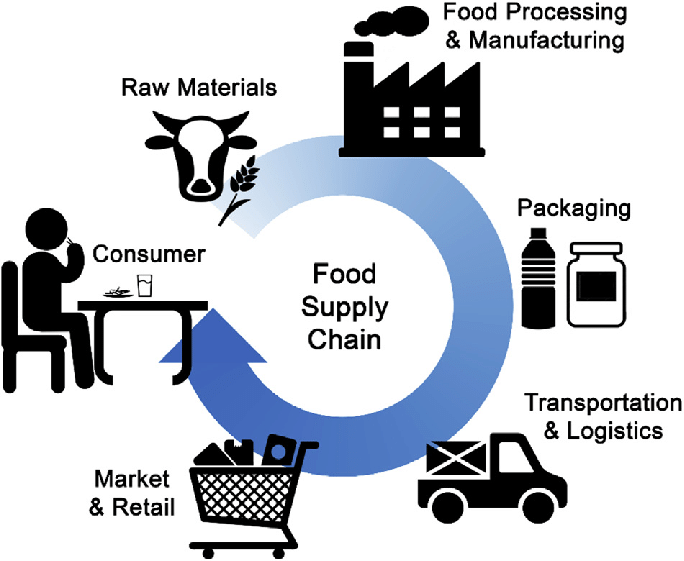
\includegraphics[width=10cm,height=8cm]{media/Food Supply Chain GS.png}
\centering
\caption{A General structure of conventional Food Supply Chain}
\end{figure}
The food industry plays a vital role in supplying the essentials and needs for numerous human activities and behaviours. Once harvested or manufactured, food should be preserved, distributed, and retailed so that it reaches its end consumers on time. According to reports, over one-third of all food produced is abandoned or wasted each year. Two-third of all food waste occurs in the supply chain, including harvesting, transporting, and warehousing. For example, fruits and vegetables, which were wasted in megatons worldwide owing to inefficient and inadequate food supply chain management (FSCM). As a result, Food supply chain management is critical in saving our food. 

The global economy relies on supply chains. Food supply chains are complicated systems with several actors. Currently, conventional records in food supply chains merely monitor and store orders and shipments, without incorporating essential features such as transparency, traceability and auditability. Furthermore, communication gaps between supply chain partners, the possibility of food fraud, rising supply chain costs and growing regulations highlight the system's inefficiencies. Tackling these hurdles will improve food quality and safety, gaining popularity among consumers. 
\subsection{Blockchain Technology}
Blockchain is a decentralised, immutable and distributed ledger that may be used to replace the traditional method of recording transactions by employing a centralised database with transactions that are validated by network nodes and recorded on a new block in the blockchain. To ensure trust and reliability across the supply chain, the stored assets must be tamper-proof. Since all of the entries maintained in a blockchain are based on a consensus reached by the overall majority of the network's peers, this distributed ledger is immutable by design and provides an auditable and transparent source of information. Blockchain technology is applied in a wide range of industries, such as banking, healthcare, IoT (Internet of Things), insurance and supply chain management. It has been demonstrated to be extremely successful in combating fraud and theft.
\\
\subsubsection{Application of Blockchain Technology in Food Supply Chain}
Blockchain technology can be applied to many industries including food supply chain which improves the supply chain efficiency by allowing organisations to conduct transactions without the intervention of third parties. The use of blockchain in the food supply chain has been gaining traction in the past few years. There are many use cases of blockchain in the food supply chain, but some of the more prominent ones include traceability, anti-counterfeiting, and transparency. These three benefits have made blockchain a popular choice for companies to choose as their method for tracking their products and services. It is easy to track and monitor a product’s history and insights into a customer's purchase. This makes fraud much harder to commit. \\

Using Blockchain to handle fruits and vegetables in the agricultural supply chain, allows farmers to participate without the involvement of intermediaries. It will also allow different stakeholders, including customers, to track and trace agricultural items as they travel through the supply chain. A blockchain-based system should record transactions relevant to the supply chain's sales and acquisitions of items. Smart contracts are self-executing contracts that transform a buyer-seller agreement into code representation. Such contracts can be used to record the terms of the negotiations and to compare the results to the agreed-upon conditions. The system is decentralised and transparent since no one entity has authority over the transaction's execution any more, offering security by promoting authenticity and immutability. \\

Digitization of the food supply chain, aided by blockchain technology, is possible by combining numerous digital technologies such as QR codes, RFID, NFC, online certification and digital signatures, sensors and actuators, mobile phones, and so on, and the Internet is the infrastructure that connects everything. Every action conducted across the food chain is logged on the blockchain, which offers an immutable means of storing information that has been accepted by all parties involved. The information obtained during each transaction is validated by the food supply network's key stakeholders, resulting in agreement among all participants. Each validated block is added to the chain of transactions, producing a permanent record of the whole process. At each level of the food supply chain, new technologies are used, and different information is written to the blockchain.
\subsubsection{Decentralised Application - DAPP}
An application that combines a smart contract and a frontend user interface is referred to as a decentralised application (dapp) and is constructed on a decentralised network. Your dapp can even contain a smart contract that was created by someone else as smart contracts on Ethereum are transparent and easily accessible, much like open APIs.
\begin{figure} [H]
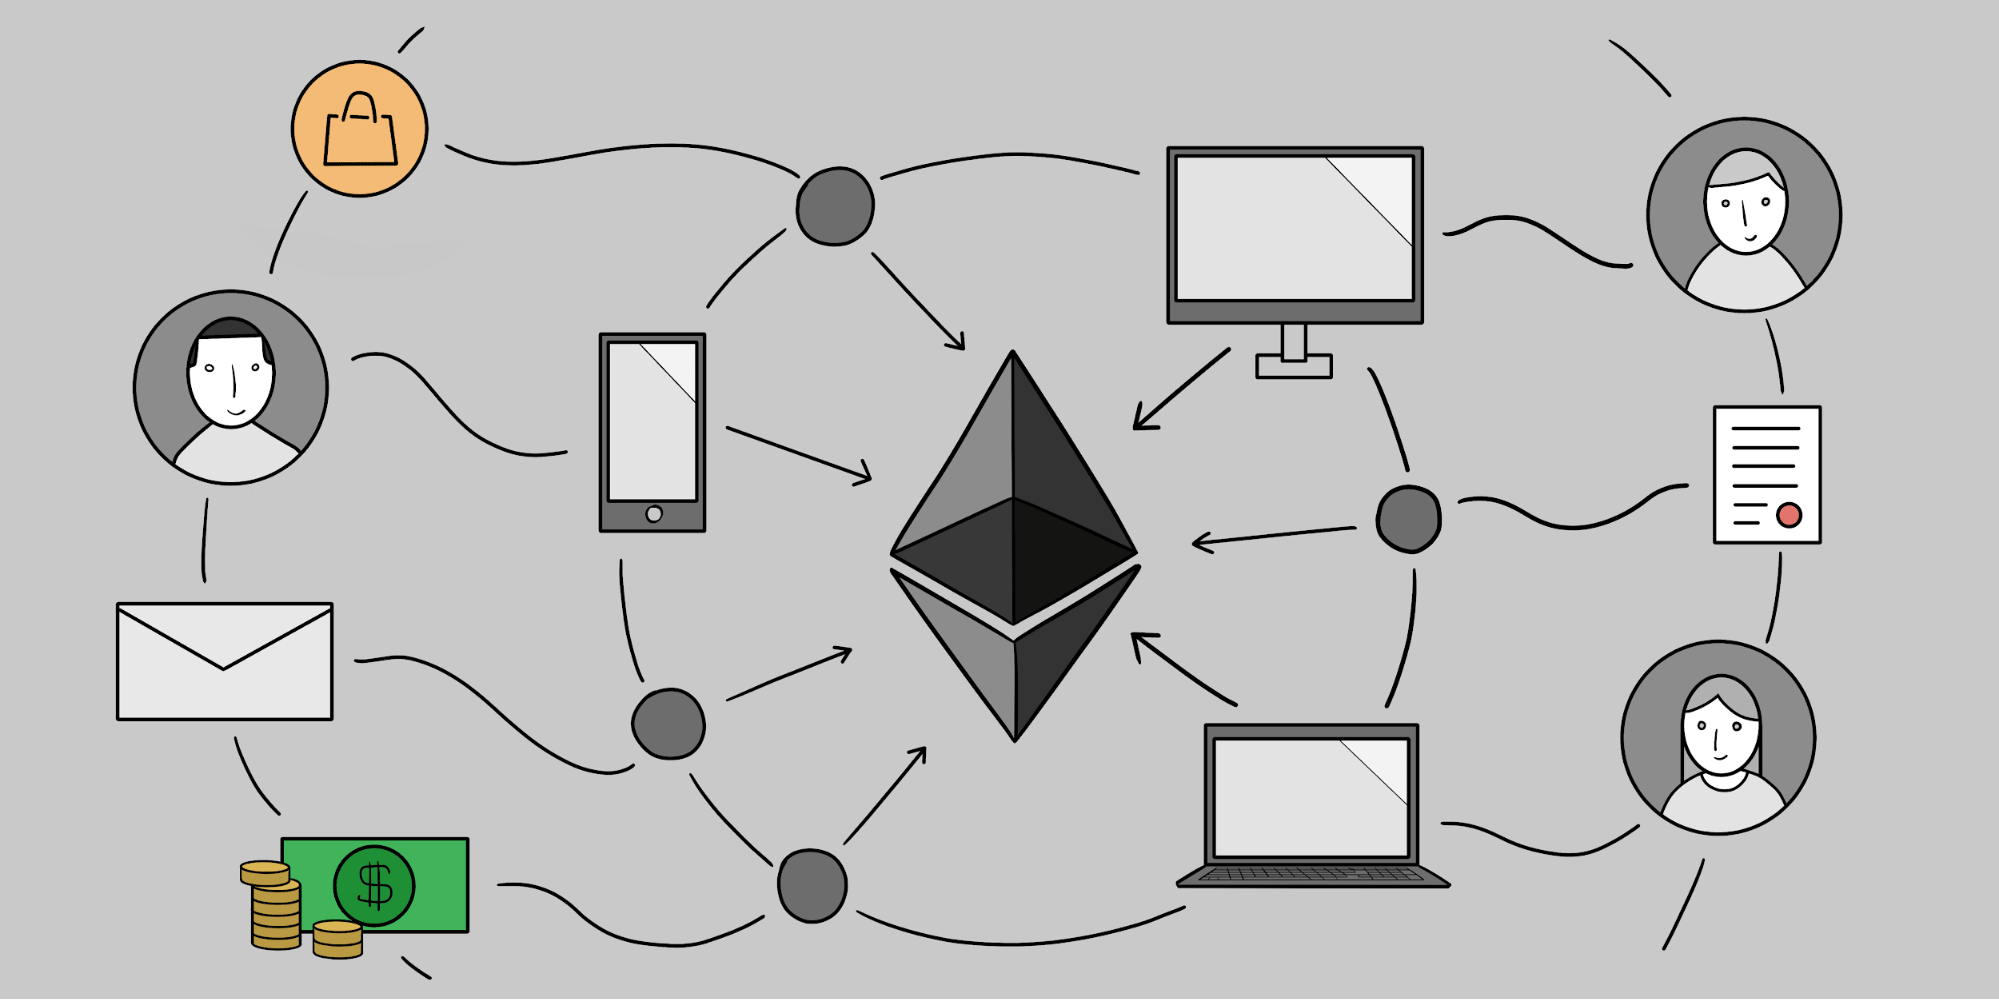
\includegraphics[width=8cm,height=6cm]{media/DAPP.png}
\centering
\caption{DAPP}
\end{figure}
Smart contract capability is available on Ethereum, a decentralised, open-source blockchain. Its native cryptocurrency is called Ether (ETH). Only Bitcoin has a larger market cap among cryptocurrencies than Ether. Programmer Vitalik Buterin came up with the idea for Ethereum in 2013. Gavin Wood, Charles Hoskinson, Anthony Di Iorio, and Joseph Lubin were further founding members of the Ethereum project. Crowdfunding for the network's development work started in 2014, and on July 30, 2015, it launched. Anyone may create decentralised applications that are permanent, irreversible, and interact with users on Ethereum. Applications for "decentralised finance" (DeFi) offer a wide range of financial services without the need for conventional financial intermediaries like banks, brokerages, or exchanges, such as enabling cryptocurrency owners to borrow money against their holdings or lend them out for interest. NFTs, which are distinctive tokens that indicate ownership of an associated asset or privilege and are acknowledged by a number of institutions, are likewise possible to generate and exchange using Ethereum.
\subsubsection{Metamask}
The Ethereum blockchain can be interacted with using the software wallet MetaMask. It enables users to interact with decentralised applications by giving them access to their Ethereum wallet via a browser extension or mobile application. A blockchain software business focused on Ethereum-based infrastructure and tools, ConsenSys Software Inc. is the creator of MetaMask. With MetaMask, users may send and receive Ethereum-based cryptocurrencies and tokens, broadcast transactions, store and manage account keys, and securely connect to decentralised applications using a suitable web browser or the built-in browser of the mobile app. Using a JavaScript plugin like Web3js or Ether to specify interactions between Metamask and Smart Contracts, developers connect Metamask to their decentralised applications. By combining numerous decentralised exchanges (DEXs) to discover the best exchange rate, the Metamask application features an integrated facility for trading Ethereum tokens.
\subsubsection{Ganache}
A personal blockchain called Ganache is used to create distributed applications for Ethereum and Corda quickly. Ganache allows you to develop, deploy, and test your dApps in a secure and deterministic environment across the whole development cycle. 

The two varieties of ganache are GUI and CLI. An Ethereum and Corda desktop application called Ganache UI is available. For Ethereum development, the ganache-cli command-line tool is provided (it was originally known as the TestRPC). 
\subsubsection{Remix IDE}
For Ethereum smart contracts, Remix IDE is one of the most popular programming environments. It can offer network-based approaches to rapidly compile and release Solidity and Vyper programmes on in-house VMs or outside Web3 service providers (such as MetaMask).
Solidity is a high-level, object-oriented language that can be used to construct smart contracts. Programs known as smart contracts control how accounts behave in the Ethereum state. Targeting the Ethereum Virtual Machine, Solidity is a curly-bracket language (EVM). C++, Python, and JavaScript have an impact on it. 
\subsection{Authenticated solution for Food Supply Chain}
In our project, we present Foodereum, an Ethereum-based authentication system for food programmes that allow organisations to record, track and authenticate food products along the supply chain. Since immutability is a virtue of the blockchain, transactions cannot be tampered or hidden because every transaction is recorded in a distributed ledger, which also can be traced and revealed to the whole network who have access to the data. This implies that anytime a product is delivered, a new receiver will be able to view the product's entire history on the blockchain network. A comprehensive performance analysis of the proposed method in terms of gas consumption has been reviewed.
\begin{figure} [H]
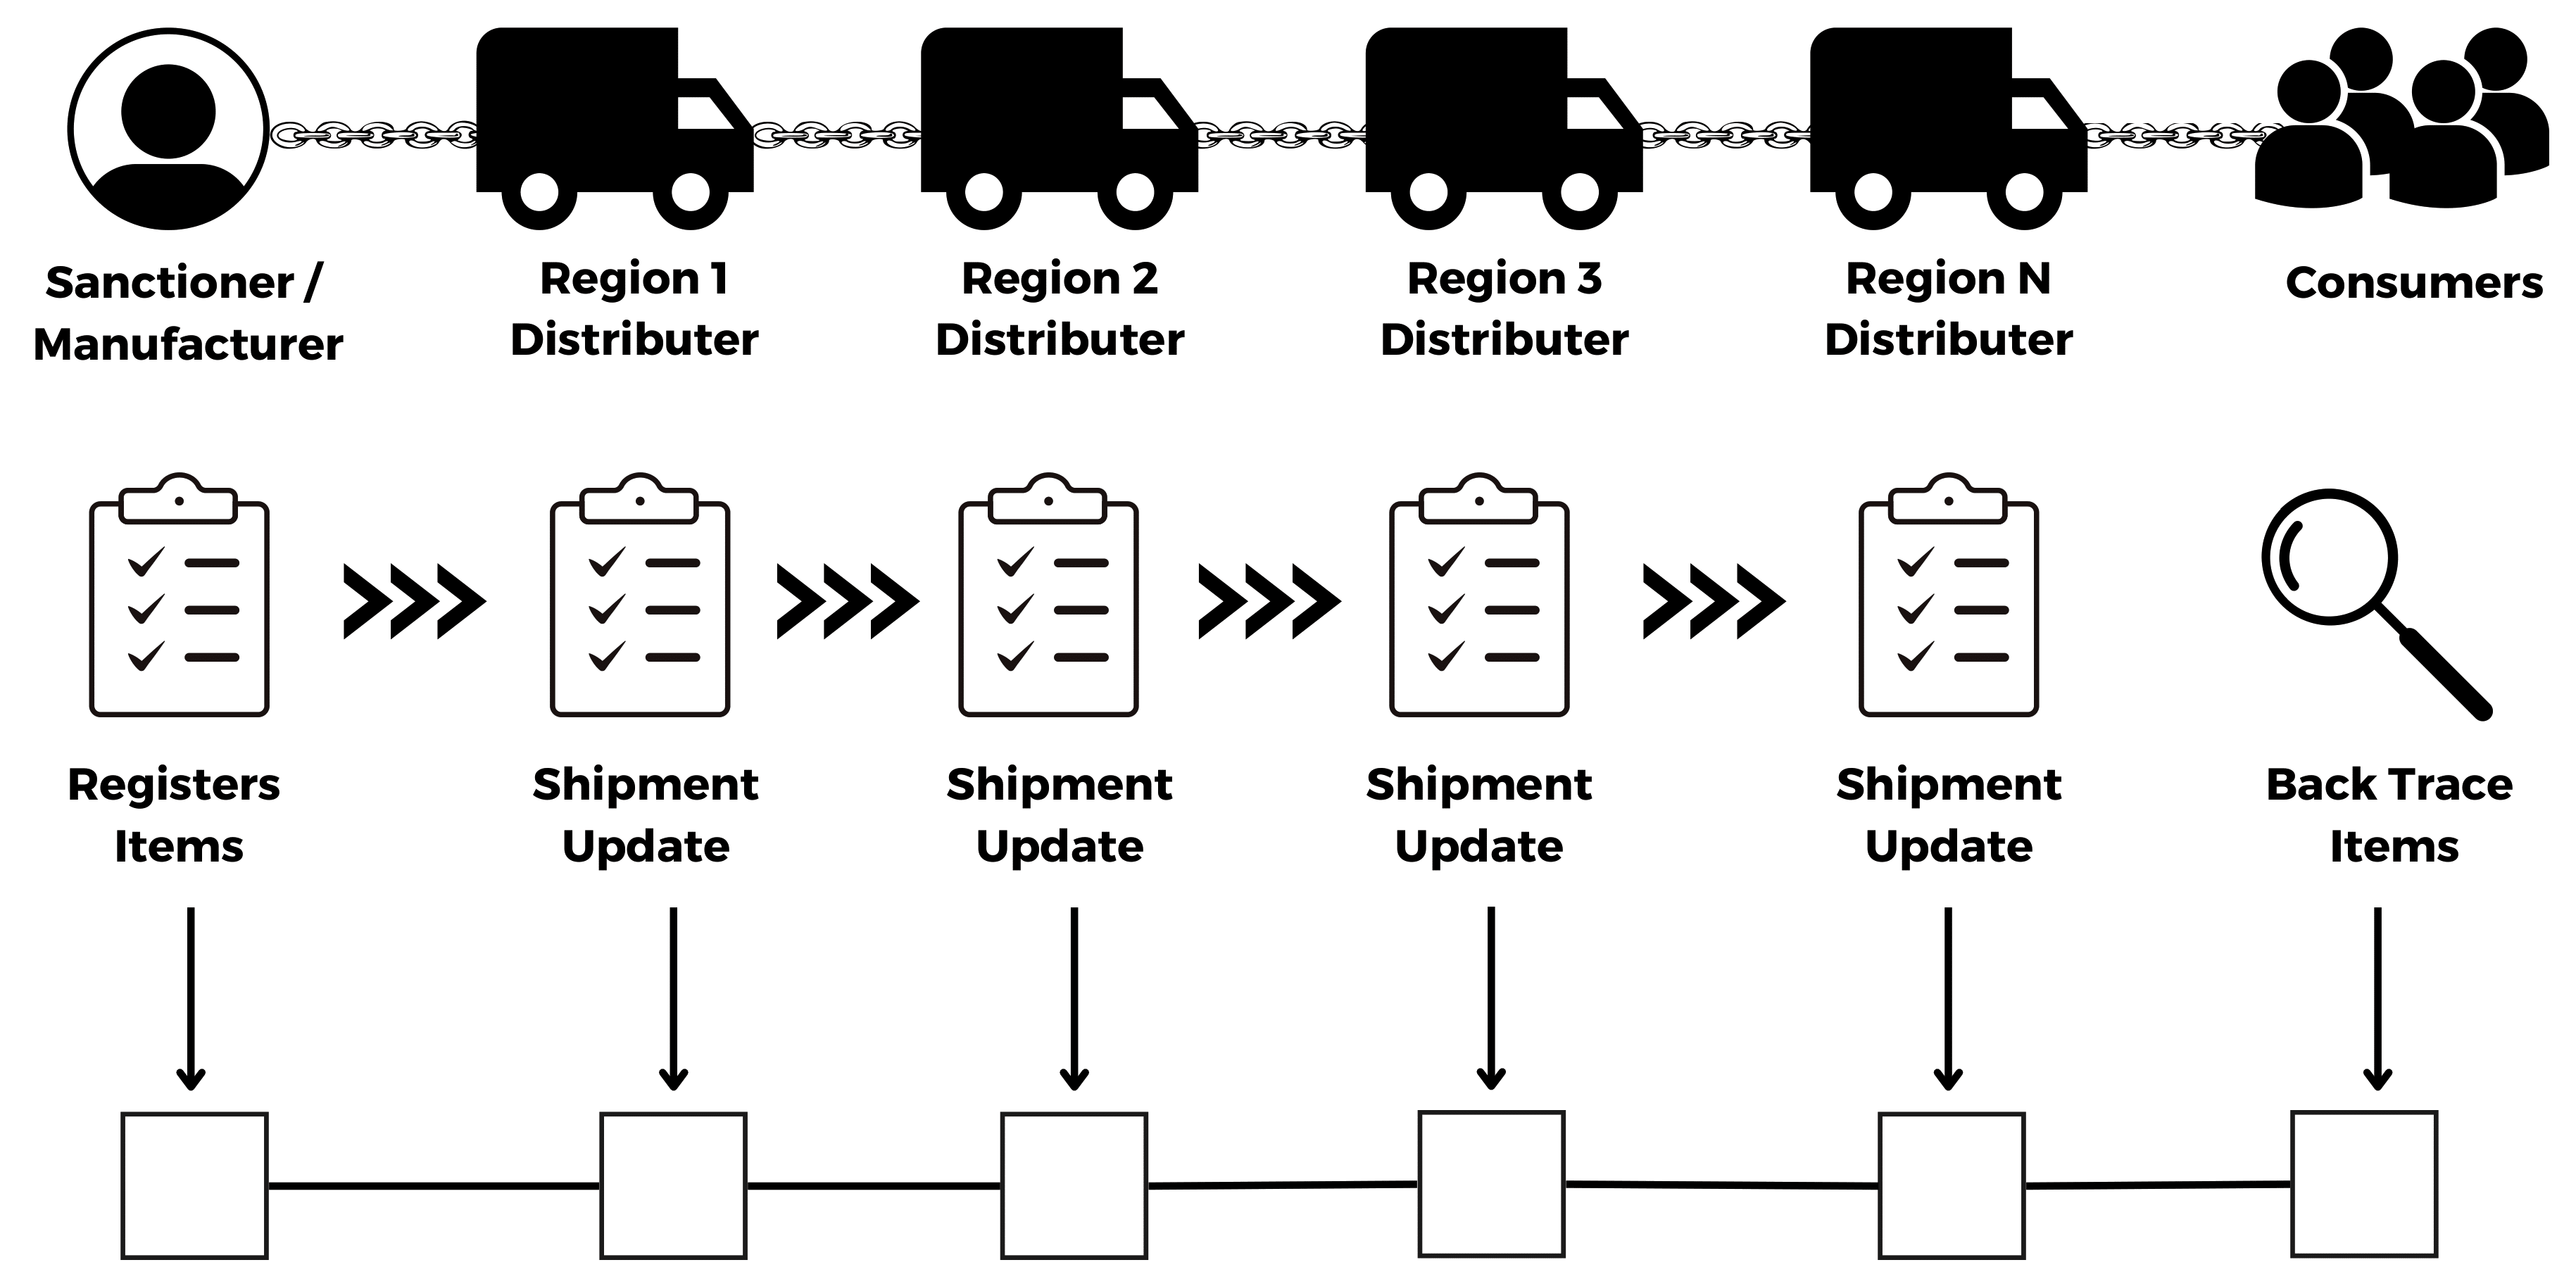
\includegraphics[width=11cm,height=7cm]{media/Sanctioner.png}
\centering
\caption{Blockchain-based food supply chain}
\end{figure}
Blockchain overcomes the difficulties by offering a balance in a sophisticated supply chain. Since there are no third parties engaged in transaction, authorisation and everything is accomplished by consensus, both users and system operators must follow a set of rules to keep the system working. In our proposed model the food products have to be authenticated upon shipment at each level or region. The authentication in the system establishes a tamper-proof environment in the supply chain, which eliminates fraudulent activities, ensures accountability of the entities involved, maintains data integrity and also the provides complete transparency in the system. As consumers seek assurance for the food they consume, an authentication system in the food supply chain, allows consumers to be treated with transparency and openness which enables them to recognise and consume high quality food. 
Figure 1.3 is a representation of the blockchain based food supply chain. 
The components of the supply chain are: 
\begin{itemize}
    \item \textbf{Sanctioner / Manufacturer:} Who is resposible for sanctioning or producing the food commodities.
    \item \textbf{Distributors}: These entities are in charge of authenticating the shipments and transporting the food commodities from place to place which are sanctioned by the Sanctioner / Manufacturer.
    \item \textbf{Consumers:} The end users who receives the food products.
\end{itemize}

Each transaction such as, the process of registering or sanctioning the food products in the network and authenticating it for the purpose of shipment will be recorded as blocks, which enables to achieve complete traceability in the system and maintain trust among the consumers in the food supply chain. \\
\subsection{Real-time Applications}
\begin{enumerate}
    \item \textbf{Government Mid-day meal scheme:} Due to a lack of transparency and quality control, there is a risk of food contamination or low quality of food items under this program. Blockchain technology may be used to address this issue since information is saved in blocks that cannot be tampered with and is visible to all blockchain network participants.
    \item \textbf{Groceries delivery:} The grocery industry finds it difficult to satisfy the growing need for transparency because of logistical issues that might lead to food waste. Blockchain may be able to resolve these problems.
    \item \textbf{Agriculture:} By enabling  traceability of information across the food supply chain, blockchain technology helps to increase food safety. It gives users a safe means to store and manage data, which makes it easier to create and use data-driven innovations for smart farming.
    \item \textbf{Import and Export businesses:} Utilizing warehouse automation and blockchain technology will help keep the supply and demand of fruits and vegetables in balance, save food from deteriorating, and increase business profitability. The vendor is no longer concerned about the import or export of fruits and vegetables. \\ \\
    \item \textbf{Food delivery or quick-commerce:} By organising all processes such as raw material procurement, order administration, meal preparation, packing, and delivery to the customer's door, blockchain can help optimise the food delivery supply chain. Operations optimization at all levels reduces expenses and saves time.
\end{enumerate} 
\subsection{Organisation of the Project Report}
The project report is organized as given below: In Chapter (2), we discuss the problem statement and our solution to the problem. The same chapter also deals with the other existing technology and the proposed solution. The Chapter that follows i.e. Chapter (3) consists of the details on the literature survey of the papers to the problem statement. In Chapter (4), we present the System Architecture in the form of System Model and Data Flow Diagram. The next chapter, Chapter (5) gives the requirements and details about the implementation of the proposed system along with the technology stack used in the project. In Chapter (6), we discuss the end result of the project. Chapter (7) concludes the paper along with a mention of the Future Enhancements. The other supporting information and the source code are gathered in the Appendix. 
\newpage
  \pagestyle{fancy}
  \thispagestyle{empty}
  \thispagestyle{plain}
  \fancyhf{}
  \lhead{Foodereum: A Blockchain-based Authenticated Solution for Food Supply Chain $|$}
  \chead{}
  \rhead{Batch No.: 41}
  \renewcommand{\headrulewidth}{0.4pt}%
  \rfoot{Page \thepage \hspace{1pt} of \pageref{LastPage}}
  \lfoot{Dept. of CSE, DSCE}
\renewcommand{\footrulewidth}{0.4pt}%
\normalsize
\section{Chapter 2: Problem Statement and Proposed Solution}
\subsection{Problem Statement}
To build an authenticated food supply chain system that provides efficient traceability, transparency of information, improves the quality and prevents wastage of food and ensures accountability of Supply Chain entities involved in the distribution of food commodities. \\
\subsection{Existing Systems}
\subsubsection{AgriBlockIoT}
\begin{figure} [H]
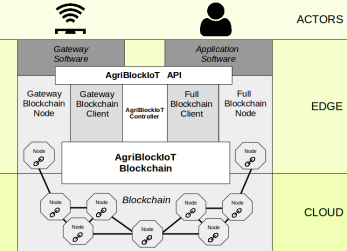
\includegraphics[width=11cm,height=7cm]{media/AgriBlockIoT.png}
\centering
\caption{AgriBlockIoT}
\end{figure}
AgriBlockIoT, a fully decentralised traceability solution for the Agriculture and Food (Agri-Food) supply chain management. By directly creating and consuming critical information from IoT devices along the supply chain and storing such data directly in its underlying blockchain. All players (including IoT devices) must be registered users of the blockchain, having the required public/private key pairs to digitally sign each action on the distributed ledger. The proposed solution ensures transparent, immutable and auditable asset tracking in a trustless environment. However, no discussion has been made of the performance study of more limited hardware designs to test the suitability of the proposed framework to applications employing real IoT devices and gateways along the Agri-Food supply chain. \\
\subsubsection{Monitoring Crop prices}
\begin{figure} [H]
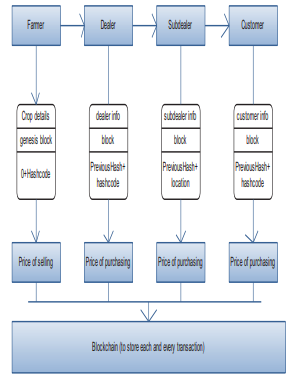
\includegraphics[width=11cm,height=16cm]{media/Supplychain_Model.png}
\centering
\caption{Monitoring Crop price}
\end{figure}
A method for monitoring crop prices in the agricultural supply chain is demonstrated using blockchain to regulate, track and execute business activities by eliminating intermediaries. The proposed solution includes automated payments and delivery proof, in which parties are compensated using cryptocurrency via smart contracts for successful product distribution. However, the approach does not address concerns such as identity authentication, enforcement, scalability, privacy standards and legislation. This solution does not use a QR code to identify items, and there is no real-time application implemented. 
\subsubsection{Reputation System}
\begin{figure} [H]
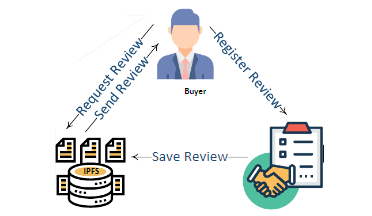
\includegraphics[width=11cm,height=7cm]{media/Reputation_System.png}
\centering
\caption{Reputation System}
\end{figure}
A blockchain-based reputation system is implemented in the Agri-Food supply chain.  It employs Ethereum smart contracts to provide trust across trade entities and to ensure that the buyer is aware of the seller's reputation before collecting data from the seller. When entities sign a smart contract for a transaction, a reputation smart contract is initiated, which provides reviews of available data sellers. The system maintains the credibility of trade entities and product quality ratings. Furthermore, because it is built on blockchain, it ensures the immutability and integrity of the recorded review. The paper also provides extensive simulation results proving that the system requires a set amount of waiting time in order to mine the transaction. Nonetheless, the waiting time is independent of input length of reviews. However there are no discussions made about how to improve the efficiency of the proposed solution, using the performance parameters. \\
\subsection{Proposed Solution}
The proposed solution uses Ethereum-based Blockchain network that provides transparency of information, improves the quality, prevents wastage and ensures accountability of Government administration in the distribution of food commodities. The food products will be Authenticated at each level along with the Geolocation by Government officials using QR codes or Product IDs, which ensures transparency and eliminates corruption in the system. The food products can be tracked using QR code or Product ID by any entity at
any time in the network. \\
We use 3 Smart Contract functionalities:
\begin{enumerate}[a)] % a), b), c), ...
    \item Sanction Products
    \item Scan \& Update Products
    \item Track Products
\end{enumerate}

In \textbf{Sanction Product}, the sanctioner can sanction food goods as a single block (Genesis Block) by providing the product name and its quantity to be sanctioned. Following sanctioning, a QR code and its associated Product ID will be generated, which may be downloaded and used to trace the product throughout the network. Once the food goods have been approved, users must be informed of the details through an inbuilt notification system. This makes tracking the food products transparent and efficient. \\

The \textbf{Scan \& Update Product} feature allows the user to authenticate food products by updating the shipment status and the product's Geo-location by either scanning the QR code or entering the product ID. Using QR code, the user can automatically update the shipment details without having to enter it manually. The Scan \& Update provides a cost-efficient, paper-free, and a time-saving alternative to traditional inventory management systems. \\

The \textbf{Track Product} feature allows the user to track the status of food products that have been updated using the Scan \& Update Product feature. Each food product may be traced in detail at each level by scanning the QR code or entering the Product ID, details include entities engaged in previous shipments, date, time and geolocation. In the event of a quality issue, the product may be tracked from its point of origin and located in no time. \\

The \textbf{Notifications} feature enables users to alert the intended recipient about the improper handling of food products or it's subpar quality. The communications would be recorded as evidence in the case of an incident. A notification describing the issue will appear when the message's recipient signs into the portal. This feature guarantees transparency and reduces the likelihood of fraud or poor management. \\

\subsection{System Requirements} 
\begin{itemize}
    \item \textbf{Ethereum:} For the simulations, an open-source blockchain technology, Ethereum, is employed. Ethereum develops decentralized apps using blockchain technology. It enables users to create smart contracts to form agreements without the intervention of a third party. 
    \item \textbf{Remix Integrated Development Environment (IDE):} Remix is used to create, execute and test smart contracts for the blockchain-based supply-chain network. Solidity is the language used in remix to create smart contracts.
    \item \textbf{Ganache:}  Ganache gives virtual accounts with a pre-defined quantity of crypto-currency in Ethers which gets deducted after each transaction. Each Ganache account has its own private key and address.
    \item \textbf{Metamask:} It is a browser plugin that works as a gateway between Ganache and Remix IDE, allowing them to communicate.
    \item \textbf{The system specifications are as follows:} Intel Core i5 8th Generation, 2.4 GHz processor, 8 GB RAM, and 1.5TB storage. 
\end{itemize}
\newpage
  \pagestyle{fancy}
  \thispagestyle{empty}
  \thispagestyle{plain}
  \fancyhf{}
  \lhead{Foodereum: A Blockchain-based Authenticated Solution for Food Supply Chain $|$}
  \chead{}
  \rhead{Batch No.: 41}
  \renewcommand{\headrulewidth}{0.4pt}%
  \rfoot{Page \thepage \hspace{1pt} of \pageref{LastPage}}
  \lfoot{Dept. of CSE, DSCE}
\renewcommand{\footrulewidth}{0.4pt}% 
\normalsize
\section{Chapter 3: Literature Survey} 
\hfill \\ 

\textbf{\emph {A. Haya R. Hasan, Khaled Salah, "Blockchain-Based Proof of Delivery of Physical Assets With Single and Multiple Transporters," IEEE Access PP(99):1-1 ( Volume: 6), 21 August 2018.}}

Due to the implementation of the proof-of-delivery technique to provide a blockchain-based proof of the distribution of real items by one or more transporters, all participating firms are honest and have dual trust security. The strategy to confirm that each unit receives the intended proportion of ether when delivered successfully must include automated ether payments. Additionally, if there is a dispute during the shipping process, there is an arbitration mechanism built into the system. The cost-effectiveness of this approach makes it suitable for both domestic and international trading in physical items. Selling digital assets, however, does not have a PoD option. For all types of physically or virtually exchanged property, this assures widespread, trustworthy, and steady transit as well as automated billing. \\ \\ \\

\textbf{\emph {B. Affaf Shahid, Umair Sarfraz, Muhammad Waseem Malik, Muhammad Sohaib Iftikhar, Abid Jamal, and Nadeem Javaid, "Blockchain-based Reputation System in Agri-Food Supply Chain," 34th International Conference on Advanced Information Networking and Applications (AINA), Luigi Vanvitelli, Caserta, Italy, February 2020.}}

This study builds a blockchain-based reputation system in the agri-food supply chain using the agri-food chain model. Using the file encryption method, it preserves the integrity and consistency of the audits enrolled through smart contracts, and provides a point by point execution inspection of the proposed system in relation to the necessary gas. While it has certain benefits, it also has some drawbacks. The results demonstrate that the framework requires special measures of holding up an excellent chance to mine the exchange, but the wait time is free of information length of audits. \\ \\

\textbf{\emph {C. Muhammad Shoaib, Ming K. Lim, Chao Wang, "An integrated framework to prioritize blockchain-based supply chain success factors," Industrial Management \& Data Systems 120(11):2103-2131, October 2020.}}

This study employs a taxonomy approach to provide an integrated framework for evaluating blockchain-based supply chain success outcomes. The goal of this assessment is to identify and prioritise factors that can have a substantial influence on the execution of blockchain-based supply chains via an integrated structure. Previous research has not attempted to focus on these factors to get the most out of the compiler's data. Key success indicators for blockchain-based supply chain technologies may be identified. However, no solution has been developed to identify impediments / challenges to effective blockchain technology deployment. \\ \\

\textbf{\emph {D. Tianhui Meng, Yubin Zhao, Katinka Wolter, Cheng-Zhong Xu , "On Consortium Blockchain Consistency: A Queueing Network Model Approach," IEEE Transactions on Parallel and Distributed Systems (Volume: 32, Issue: 6), 08 January 2021.}}

This study examines the consistency attributes of consortium blockchain technologies. The success of the fundamental processes in blockchain consensus can be evaluated using the suggested method. The framework is employed in the hyperledger fabric system to retrieve crucial elements of the blockchain network. It uses the raft consensus algorithm, which has a number of benefits, including improved scalability, the isolation of trust presumptions from purchasing criteria and purchasing, support for non-deterministic smart contracts, partitioning of smart-contract programmes and data across several nodes, with its use of modular consensus adoption. However, the suggested method is not the best for examining public blockchains because PoW imposes a lag that regulates the consensus mechanism and is highly variable. The model ignores the warm-up period and business waiting time in favour of looking at the stable distribution of the consortium blockchain system. \\ \\ \\ \\ \\

\textbf{\emph {E. Jiang Duan, Chen Zhang, Yu Gong, Steve Brown and Zhi Li, "A Content-Analysis Based Literature Review in Blockchain Adoption within Food Supply Chain," International Journal of Environmental Research and Public Health 17(5):1784, March 2020.}}

This study employs a blockchain model based on hyperledger fabric to conduct a literature review which is based on content analysis of blockchain usage in food supply chains. It employs consensus algorithms to improve food discernibility, data clarity, and review efficacy. However, this provides more experimental evidence than speculations. Different food items may necessitate a distinct supply chain. \\

\textbf{\emph {F. Miguel Pincheira Caro, Muhammad Salek Ali, Massimo Vecchio, Raffaele Giaffreda, "Blockchain-based Traceability in Agri-Food Supply Chain Management: A Practical Implementation," 2018 IoT Vertical and Topical Summit on Agriculture - Tuscany (IOT Tuscany), 07 June 2018.}}

The main goal of the system's research and development is AgriBlockIoT, a completely decentralised tracking solution for tracking the agri-food supply chain. The suggested system, in particular, can use either the publically available blockchain implementations of Ethereum and can include a variety of IoT sensor devices. AgriBlockIoT offers open and auditable asset tracking by instantly creating, gathering, and storing vital data from IoT devices all throughout the supply chain and the underlying blockchain. It is consensus-based and uses an open provenance approach. Open, fault-tolerant, invariable, and auditable records could be made available by the suggested system. \\

\textbf{\emph {G. Ahmed Alketbi, Qassim Nasir, Manar Abu Talib, "Blockchain for Government Services – Use Cases, Security Benefits and Challenges," 2018 15th Learning and Technology Conference (L\&T), 25-26 Feb. 2018.}}

This research examines the various blockchain government services, including applications, security features, and restrictions, using Random-Sample Elections models. It makes use of the consensus algorithm, which has various benefits, including more dispersed, cost-effective, and voluntary delivery of government services. There is a lot of potential in using blockchain technology to provide smart government services. While it has certain benefits, it also has some drawbacks, such as failing to emphasise security enhancements and issues with applying blockchain in IoT environments.

\textbf{\emph {H. Shangping Wang, Xixi Tang, Yaling Zhang, Juanjuan Chen, "Auditable Protocols for Fair Payment and Physical Asset Delivery Based on Smart Contracts," IEEE Access PP(99):1-1 ( Volume: 7), 08 August 2019.}}

In this study, a smart contract-based traceable mechanism for equitable financing and physical asset allotment between retailers, clients, and logistics firms is investigated. The suggested protocol makes use of blockchain to address network dependability challenges. This has the benefit of being transparent, unambiguous, secure, and verifiable. It employs a shopping model, however the bulk of studies in existence only address payments or asset delivery, failing to provide clients with a thorough shopping model. The study shows that the exact same consensus method is required for global nodes in a decentralised network to agree. Based on the consensus algorithm, this strategy chooses practical byzantine fault tolerance consensus approaches and is constructed on a permissioned chain with a significant level of decentralisation. The suggested solution combines high performance, security, and scalability with openness, simplicity, validity, and credibility by using a distributed network transaction system. Transaction costs and hazards for participants are reduced. The technique, which depends on the trust of the merchant, does not, however, address how consumers may ensure the quality and usability of the goods they purchase. Therefore, the reputation of the service will be the subject of our next research study. \\

 
\textbf{\emph {I. Khaled Salah, Nishara Nizamuddin, Raja Jayaraman, Mohammad Omar, "Blockchain-Based Soybean Traceability in Agricultural Supply Chain," IEEE Access ( Volume: 7), 20 May 2019.}}

To establish soy blockchain-based traceability in the agricultural supply chain, this work employs a food processing and tracking methodology. An intermediate that uses smart contract algorithms and improved practical Byzantine Fault Tolerance Algorithms (iPBFTs) to give centralised permissions while also increasing transaction record integrity, reliability, efficiency, and security. It also allows for consistent and decentralised supply chain traceability. The evidence of payment and delivery, however, will not be automated if the cryptocurrency is given to the parties in a centralised manner automated by smart contracts following successful physical delivery and dispute settlement of the crop or product. \\ \\
 
 
\textbf{\emph {J. Saveen A. Abeyratne, Radmehr P. Monfared, "Blockchain Ready Manufacturing Supply Chain Using Distributed Ledger," IJRET: International Journal of Research in Engineering and Technology eISSN: 2319-1163 $|$ pISSN: 2321-7308 $|$ Volume: 05 Issue: 09, September 2016.}}

This paper aims to build a blockchain-compatible manufacturing supply chain with distributed ledger using a blockchain-based paradigm. It employs a cryptographic technique to increase system traceability and maximise transparency of system parts while ensuring data integrity and security. It also makes it easier to collect enormous volumes of data on manufactured goods and users, which is beneficial to a wide range of researchers, companies, individuals and governments. However, it needs particular IT infrastructure, such as internet connectivity. This is currently impractical for certain faraway raw material suppliers. Digital profiles must be updated on a regular basis, either manually or automatically. To incentivize the blockchain and speed the pace of business operations, smart contracts must be built and incorporated into the system. Furthermore, the performance of such systems may be a hindrance in implementing the proposed approach.
 
\newpage
  \pagestyle{fancy}
  \fancyhf{}
  \lhead{Foodereum: A Blockchain-based Authenticated Solution for Food Supply Chain $|$}
  \chead{}
  \rhead{Batch No.: 41}
  \rfoot{Page \thepage \hspace{1pt} of \pageref{LastPage}}
  \lfoot{Dept. of CSE, DSCE}
\renewcommand{\footrulewidth}{0.4pt}% 
\normalsize
\begin{figure} [H]
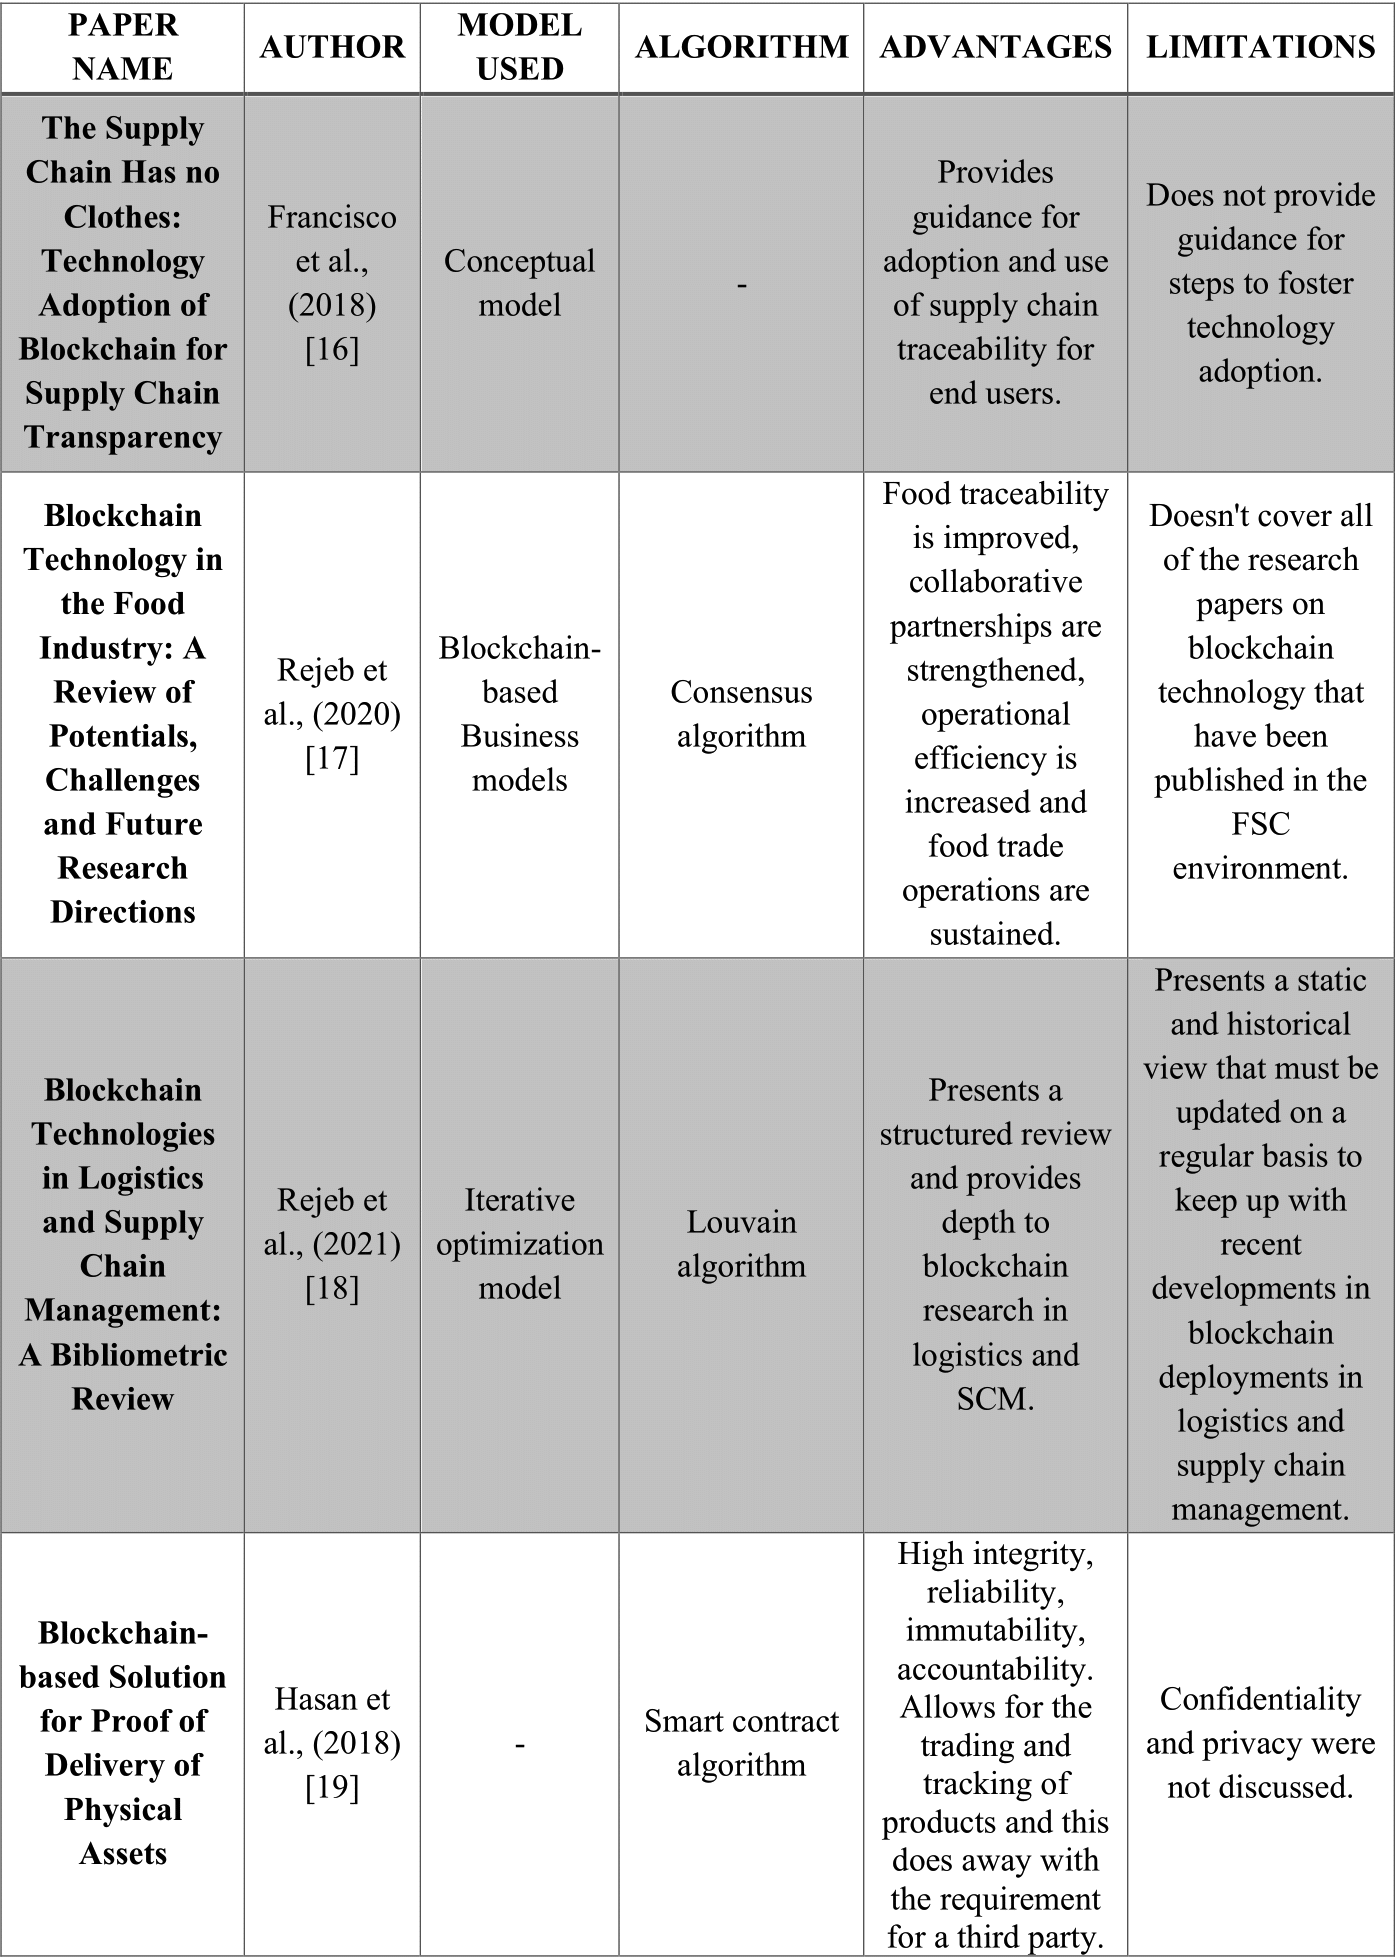
\includegraphics[width=17cm]{media/Lit_Survey_1.png}
\centering
\end{figure}
\begin{figure} [H]
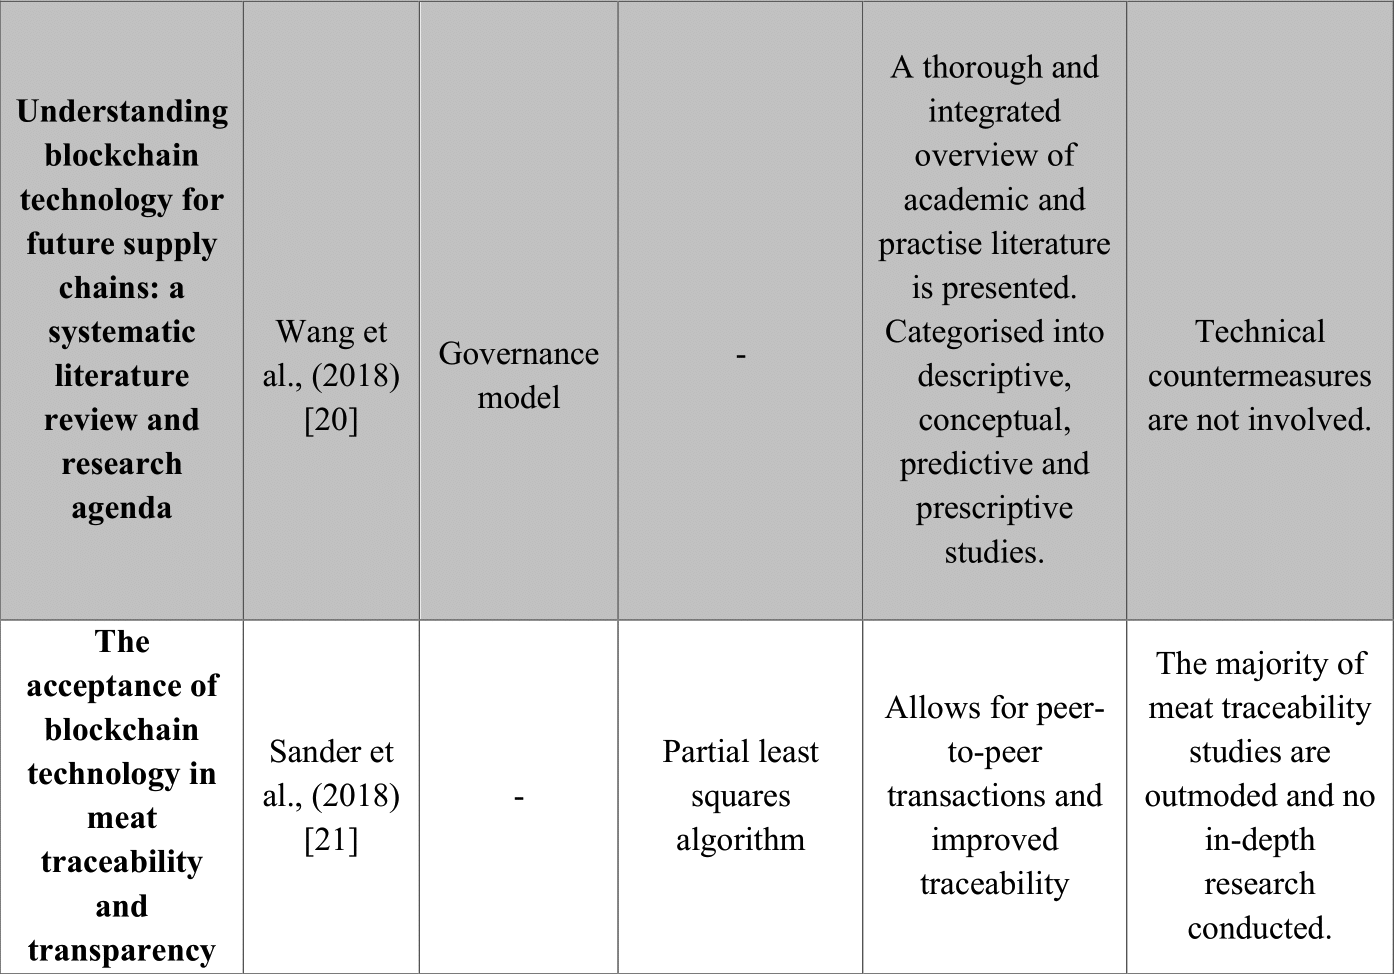
\includegraphics[width=17cm]{media/Lit_Survey_2.png}
\centering
\end{figure}
\newpage
  \pagestyle{fancy}
  \thispagestyle{empty}
  \thispagestyle{plain}
  \fancyhf{}
  \lhead{Foodereum: A Blockchain-based Authenticated Solution for Food Supply Chain $|$}
  \chead{}
  \rhead{Batch No.: 41}
  \renewcommand{\headrulewidth}{0.4pt}%
  \rfoot{Page \thepage \hspace{1pt} of \pageref{LastPage}}
  \lfoot{Dept. of CSE, DSCE}
\renewcommand{\footrulewidth}{0.4pt}%
\section{Chapter 4: Architecture and Design} 
\subsection{System Architecture}
\subsubsection{System Model}
We provide our system model in this section, which is used to identify and analyse the system's key components, as well as their linkages and interactions. Our proposed model is a three-layered architecture with supply chain entities in the first layer, a smart contract and notification system in the second layer, and a simulated Ethereum blockchain in the third layer. 

The shipping details which are generated from the first layer through the supply chain entities are stored in a ledger on the second layer, through smart contract, the shipping events are then recorded on the blockchain in the third layer. The transactions which are stored in the ledger at the second layer contain the hashes of the blocks, which helps in efficient storage management. 

At second layer, a smart contract is employed which holds the core functionalities and a strict control access mechanism is also integrated on the basis of the roles of the supply chain entities, which determines who has access to read or write the data on the blockchain. A notification system is also a part of second layer, which is accounted for establishing communication and enabling trust between entities. This feature also acts as a reputation system, which is in charge of handling discrepancies or miscommunications between entities. The third layer in the system responsible for storing the data in the blockchain which is produced from layer two.
\begin{figure} [H]
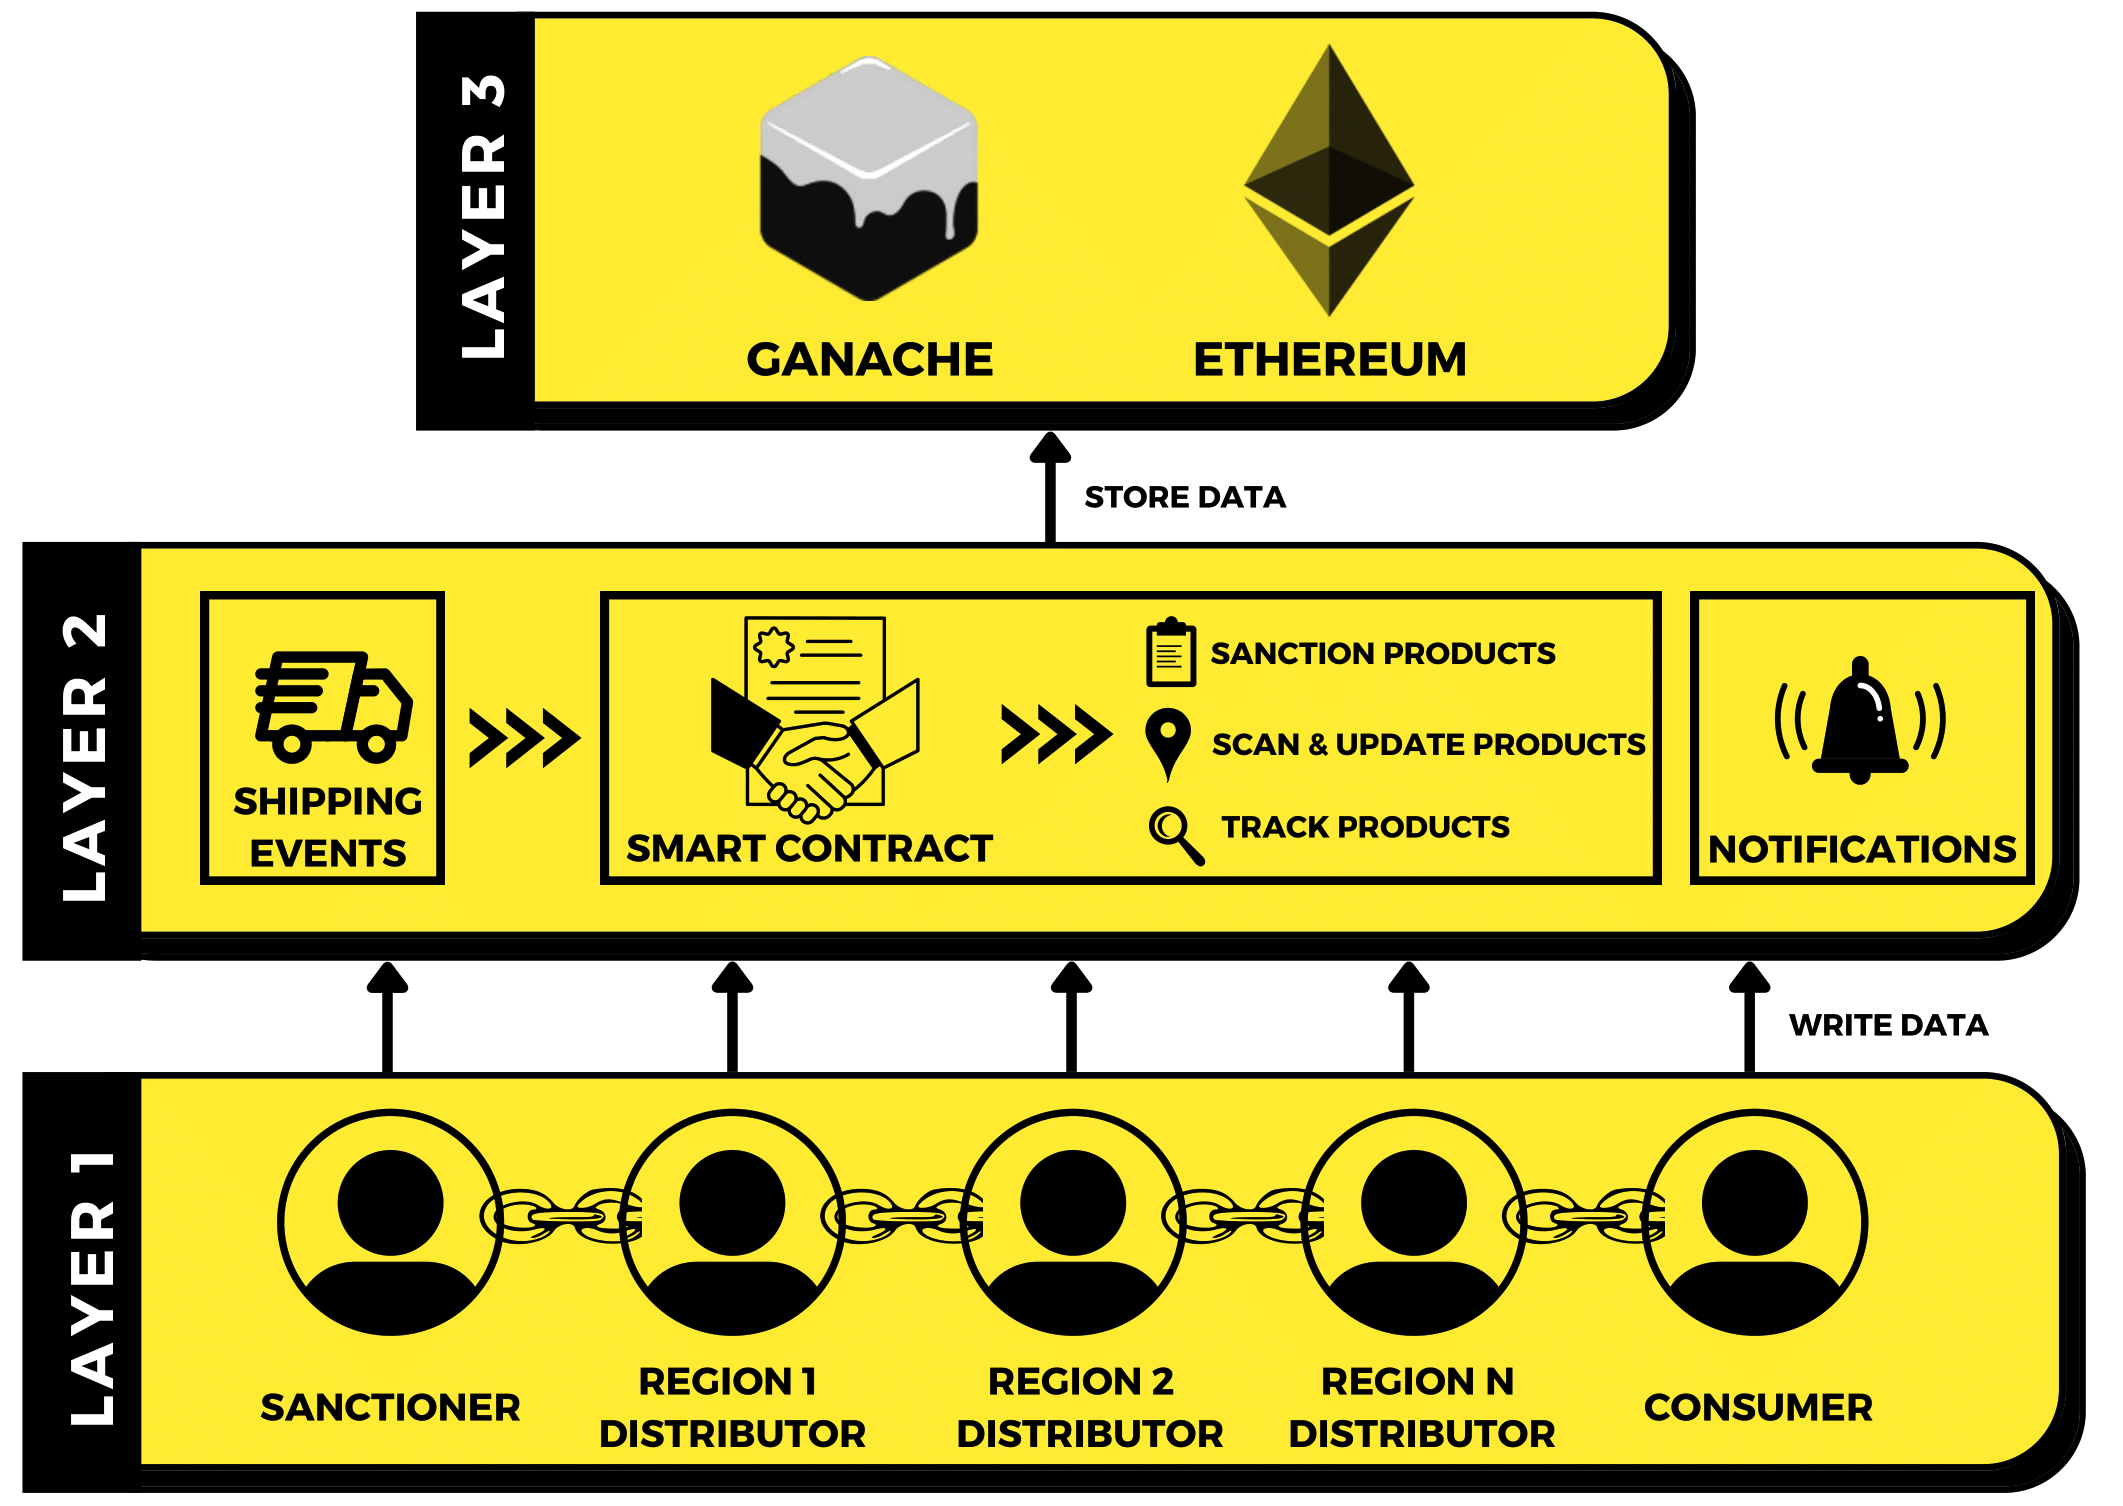
\includegraphics[width=12cm,height=8cm]{media/System_model.png}
\centering
\caption{System Model}
\end{figure}
\textbf{Layer 1} consists of the several supply chain entities who communicate via the smart contract and act according to their roles. They are:
\begin{itemize}
    \item \textbf{Sanctioner:} The only person who has authority to sanction food commodities to the Consumers. Thus, a genesis block will be mined at the time of registering the food commodities in the system.
    \item \textbf{Region-wise Distributors:} The distributors are in charge of authenticating the shipments at each level which tends to record accurate data upon receiving the physical package and transporting the package from place to place. 
    \item \textbf{Consumers:} The end users who receives the food commodities.
\end{itemize}

\textbf{Layer 2}  consists of shipping events, a smart contract and a notification system. 
As the sanctioner registers the food commodities to the consumers, the commodities have to be shipped from place to place. In that context, the shipping events in the layer 2 are the details of every shipment which are authenticated by the distributors at their region across the supply chain. These shipping events are then recorded on the blockchain which can be accessed by the entities to track shipment status of the food commodities. 

A self-executing Smart contract which is present in the layer 2 of our system, contains three prominent functions which enables the entities to interact in the supply chain. The three functions are: 

\textbf{Sanction products ( ):} In Sanction Product, the sanctioner can sanction food commodities as a single block (Genesis Block). The function accepts the name of the product and its quantity to be sanctioned as the input. Following sanctioning, a QR code and its associated Product ID will be generated, which may be downloaded and used to trace the product throughout the network. Once the food goods have been approved, users must be informed of the details through an inbuilt notification system. This makes tracking the food products transparent and efficient.  \\

\textbf{Scan \& Update Products ( ):} The Scan \& Update Product feature allows the user to authenticate food products by updating the shipment status and the product's Geo-location by either scanning the QR code or entering the product ID. This function takes Product ID and the Geo-location as the inputs. Using QR code, the user can automatically update the shipment details without having to enter it manually. The Scan Update feature provides a cost-efficient, paper-free, and a time-saving alternative to traditional inventory management systems. 

\textbf{Track Products ( ):} The Track Product feature allows the user to track the status of food products that have been updated using the Scan \& Update Product feature. This function accepts the Product ID as the input. Each food product may be traced in detail at each level by scanning the QR code or entering the Product ID, details include entities engaged in previous shipments, date, time and geolocation. In the event of a quality issue, the product may be tracked from its point of origin and located in no time. This feature ensures complete traceability and transparency in the system. \\

A \textbf{Notification system} is also a part of second layer, which is accounted for establishing communication and enabling trust between entities. The Notification system also acts as a reputation system which is in charge of handling discrepancies or miscommunications between entities as any entity can communicate with any other entities in the chain to solve or raise issues. This feature also helps Food Sanctioners to assure the authenticity and reliability of their supplies by tracking tampering attempts as the food commodities flows through the supply chain. \\

At \textbf{Layer 3} , the data or the shipping events which are produced by the supply chain entities from layer two are stored in the blockchain against their roles / profiles. The transactional data which are stored in the ledger at the second layer contain the hashes which points to the blocks of the Ethereum blockchain, these transactional data are stored as metadata to overcome the limitations of a storage unit, this helps in efficient storage management. Due to the incorporation of a strict control access mechanism in the system, the access to read or write the data on the blockchain on the basis of the roles of the entities, ensures that the network's privacy and confidentiality are protected. 
\newpage
  \pagestyle{fancy}
  \fancyhf{}
  \lhead{Foodereum: A Blockchain-based Authenticated Solution for Food Supply Chain $|$}
  \chead{}
  \rhead{Batch No.: 41}
  \renewcommand{\headrulewidth}{0.4pt}%
  \rfoot{Page \thepage \hspace{1pt} of \pageref{LastPage}}
  \lfoot{Dept. of CSE, DSCE}
\renewcommand{\footrulewidth}{0.4pt}%
\normalsize
\subsubsection{Data Flow Diagram}
\begin{figure} [H]
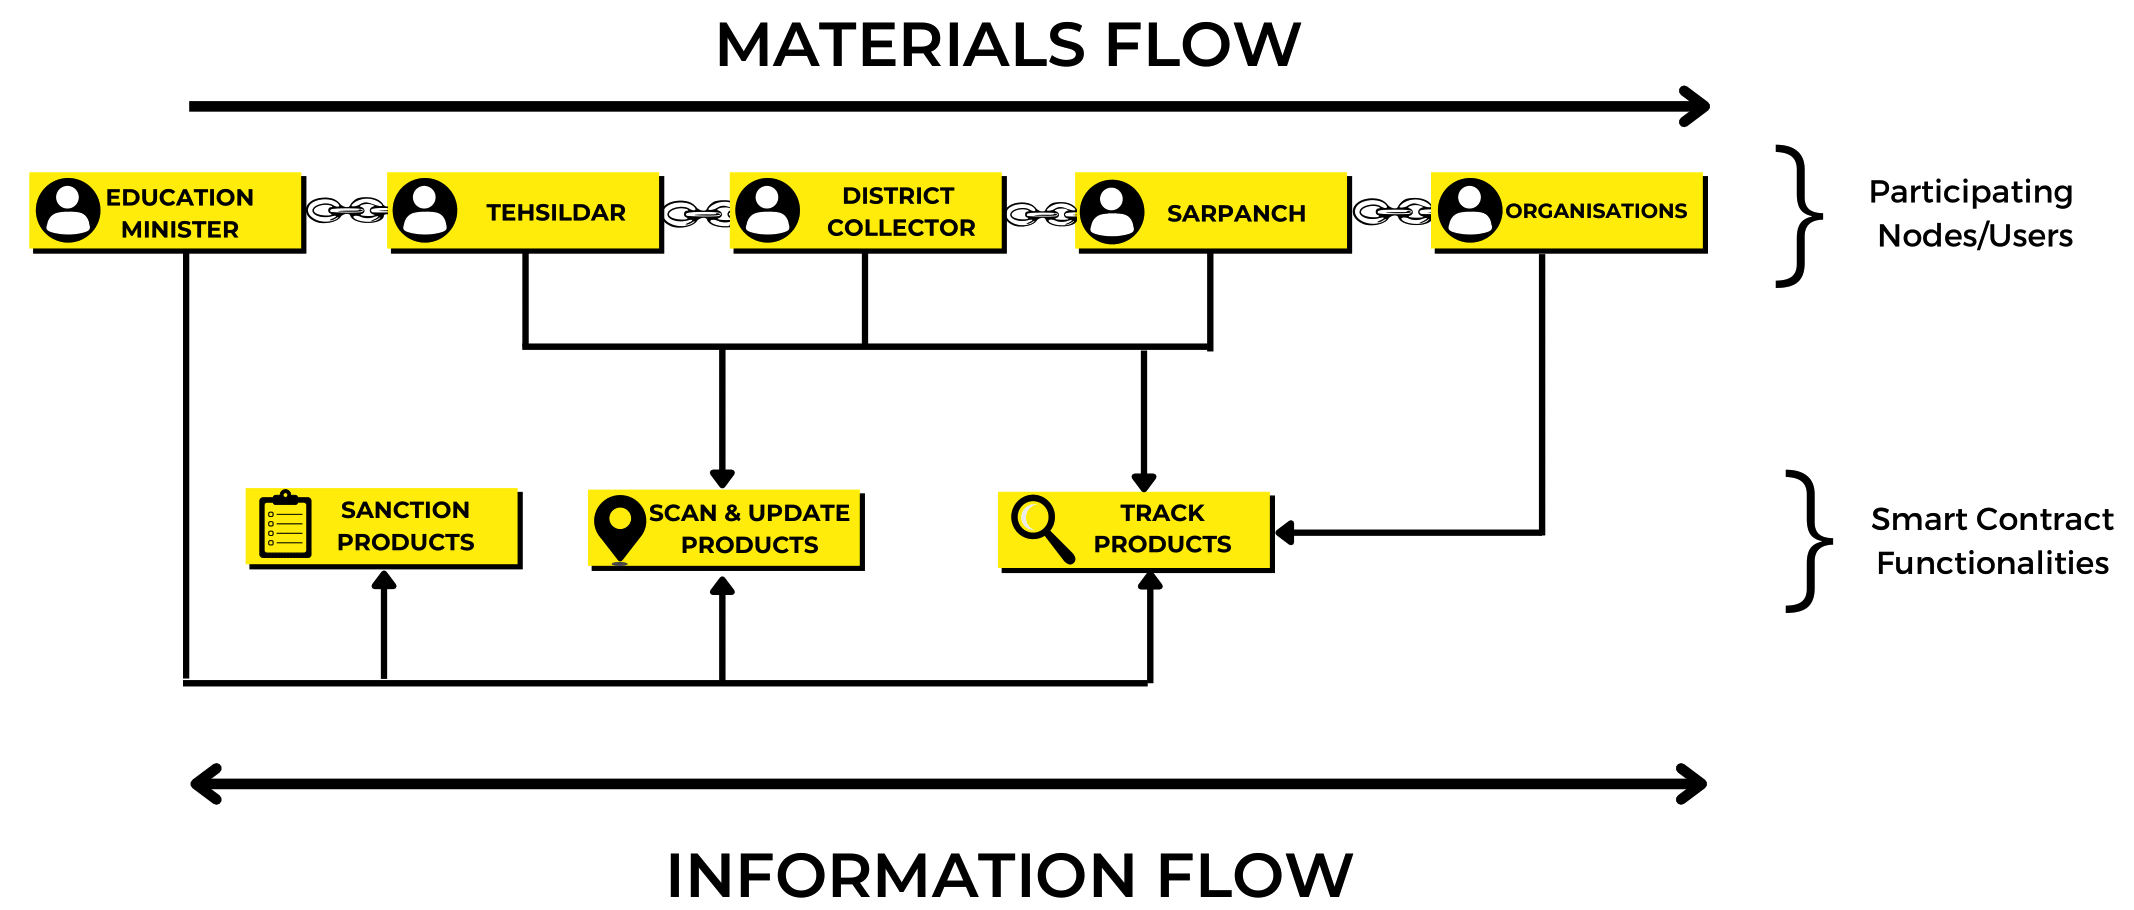
\includegraphics[width=18cm,height=10cm]{media/Data_flow.png}
\centering
\caption{Data Flow Diagram}
\end{figure}
Figure 4.2 represents the Data flow diagram where several supply chain entities communicate via the smart contract and act according to their roles. The Education Minister act as the chief sanctioner who is responsible for sanctioning the food commodities. The Tehsildar, District Collector and Sarpanch act as the region-wise distributors who authenticates the shipment at each level and finally sends the package to the organisations or the consumers. The food package is distributed in a linear fashion from the Education Minister to the Consumer via the Tehsildar, District Collector and Sarpanch representing the Material flow. At each level the package is authenticated and the details are stored in blocks, which can be tracked by any entity at any level using QR code or product ID. This information can be bidirectional representing the Information flow.
\newpage
  \pagestyle{fancy}
  \thispagestyle{empty}
  \thispagestyle{plain}
  \fancyhf{}
  \lhead{Foodereum: A Blockchain-based Authenticated Solution for Food Supply Chain $|$}
  \chead{}
  \rhead{Batch No.: 41}
  \renewcommand{\headrulewidth}{0.4pt}%
  \rfoot{Page \thepage \hspace{1pt} of \pageref{LastPage}}
  \lfoot{Dept. of CSE, DSCE}
\renewcommand{\footrulewidth}{0.4pt}%
\normalsize
\newpage
  \pagestyle{fancy}
  \thispagestyle{empty}
  \thispagestyle{plain}
  \fancyhf{}
  \lhead{Foodereum: A Blockchain-based Authenticated Solution for Food Supply Chain $|$}
  \chead{}
  \rhead{Batch No.: 41}
  \renewcommand{\headrulewidth}{0.4pt}%
  \rfoot{Page \thepage \hspace{1pt} of \pageref{LastPage}}
  \lfoot{Dept. of CSE, DSCE}
\renewcommand{\footrulewidth}{0.4pt}%
\normalsize
\section{Chapter 5: Implementation} 
\subsection{Implementation Platforms}
\subsubsection{Hardware}
\begin{itemize}
    \item \textbf{Processor:} Intel Core i5 8th Generation, 2.4 GHz processor
    \item \textbf{RAM:} 8 GB 
    \item \textbf{Storage:} 1.5 TB 
\end{itemize}
\subsubsection{Software}
\begin{itemize}
    \item \textbf{Operating System:} Windows (10) (64bit) or MacOS
    \item \textbf{Software Used:} Ganache, Metamask, Remix IDE, MAMP
    \item \textbf{Programming Languages:} Solidity
    \item \textbf{Server:} Apache
\end{itemize}
\subsection{Implementation Details}
\subsubsection{Architectural Diagram}
\begin{figure} [H]
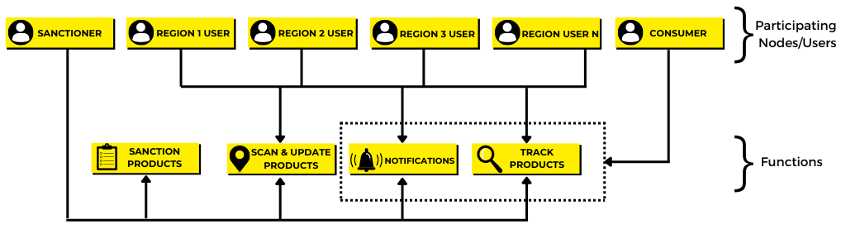
\includegraphics[width=17cm]{media/Foodereum_Arc.png}
\centering
\caption{Foodereum Architecture}
\end{figure} 
Figure 5.1 depicts how various users in the supply chain have access to different functionalities. Out of all the users in the supply chain, only the sanctioner has the authority to sanction a product. The features that the sanctioner may access are Sanction Product, Scan and Update Product, Track Product, and Notification. Users in Regions 1 through Region N are responsible for scanning delivered products and updating data on the blockchain. This helps authenticate each product on the blockchain and holds all users accountable for the safety of the product. They can also check the product's status using the Track Product feature. By using the notification feature, a user can send a message to other users informing them that the product is of low quality or missing. Only two functions are available to the consumer: Track Product and Notification.
\begin{figure} [H]
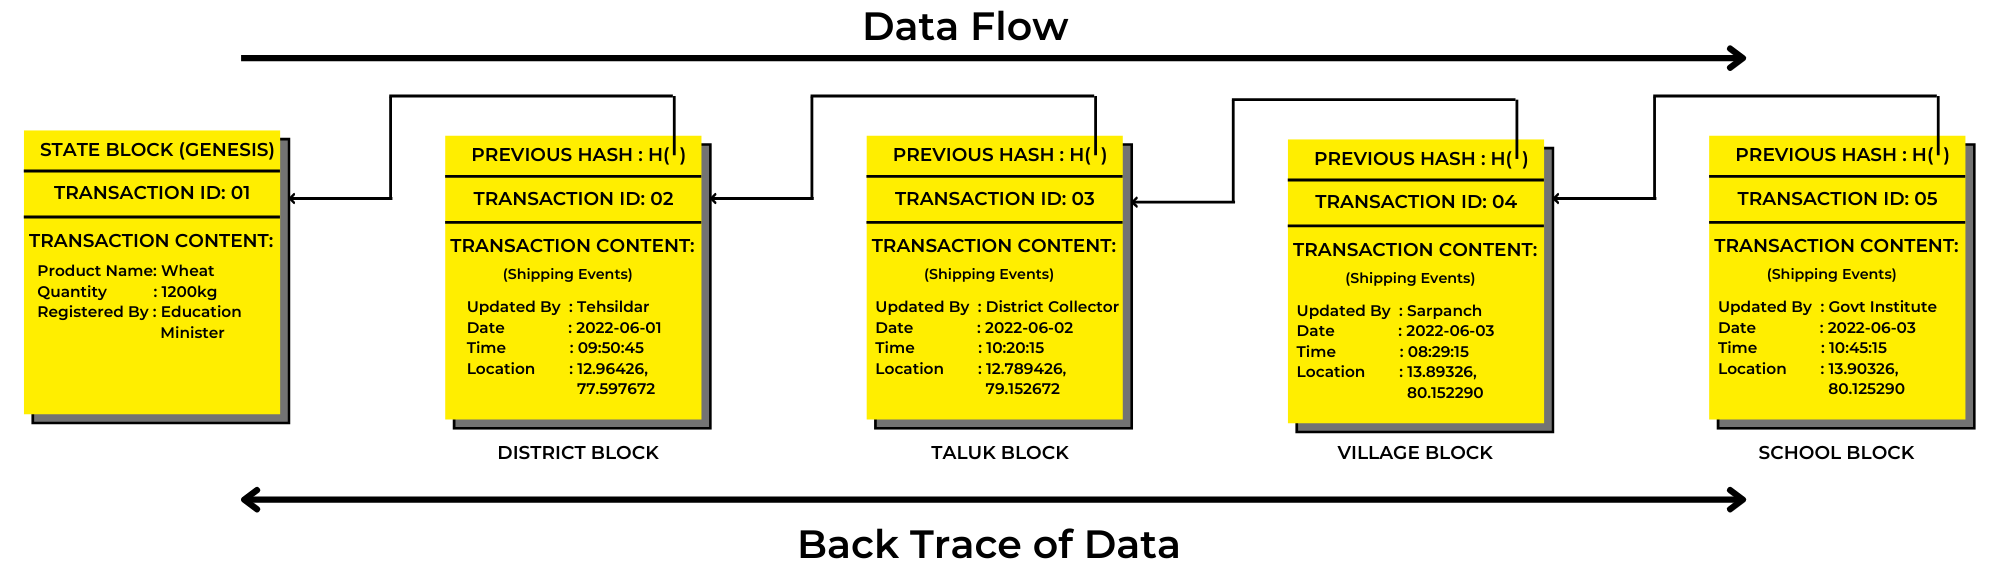
\includegraphics[width=17cm]{media/Blocks.png}
\centering
\caption{General skeletal structure of Blocks}
\end{figure}
The data flow between distinct regional blocks is depicted in Figure 5.2. Each block provides the data for a specific region that the user has given. The block contains information on who updated it, as well as the date, time, and location. Each block contains a distinct transaction ID that makes it easier to identify the original source of data.
\newpage
  \pagestyle{fancy}
  \fancyhf{}
  \lhead{Foodereum: A Blockchain-based Authenticated Solution for Food Supply Chain $|$}
  \chead{}
  \rhead{Batch No.: 41}
  \renewcommand{\headrulewidth}{0.4pt}%
  \rfoot{Page \thepage \hspace{1pt} of \pageref{LastPage}}
  \lfoot{Dept. of CSE, DSCE}
\renewcommand{\footrulewidth}{0.4pt}%
\normalsize
\subsubsection{Backend Integration}
\begin{figure} [H]
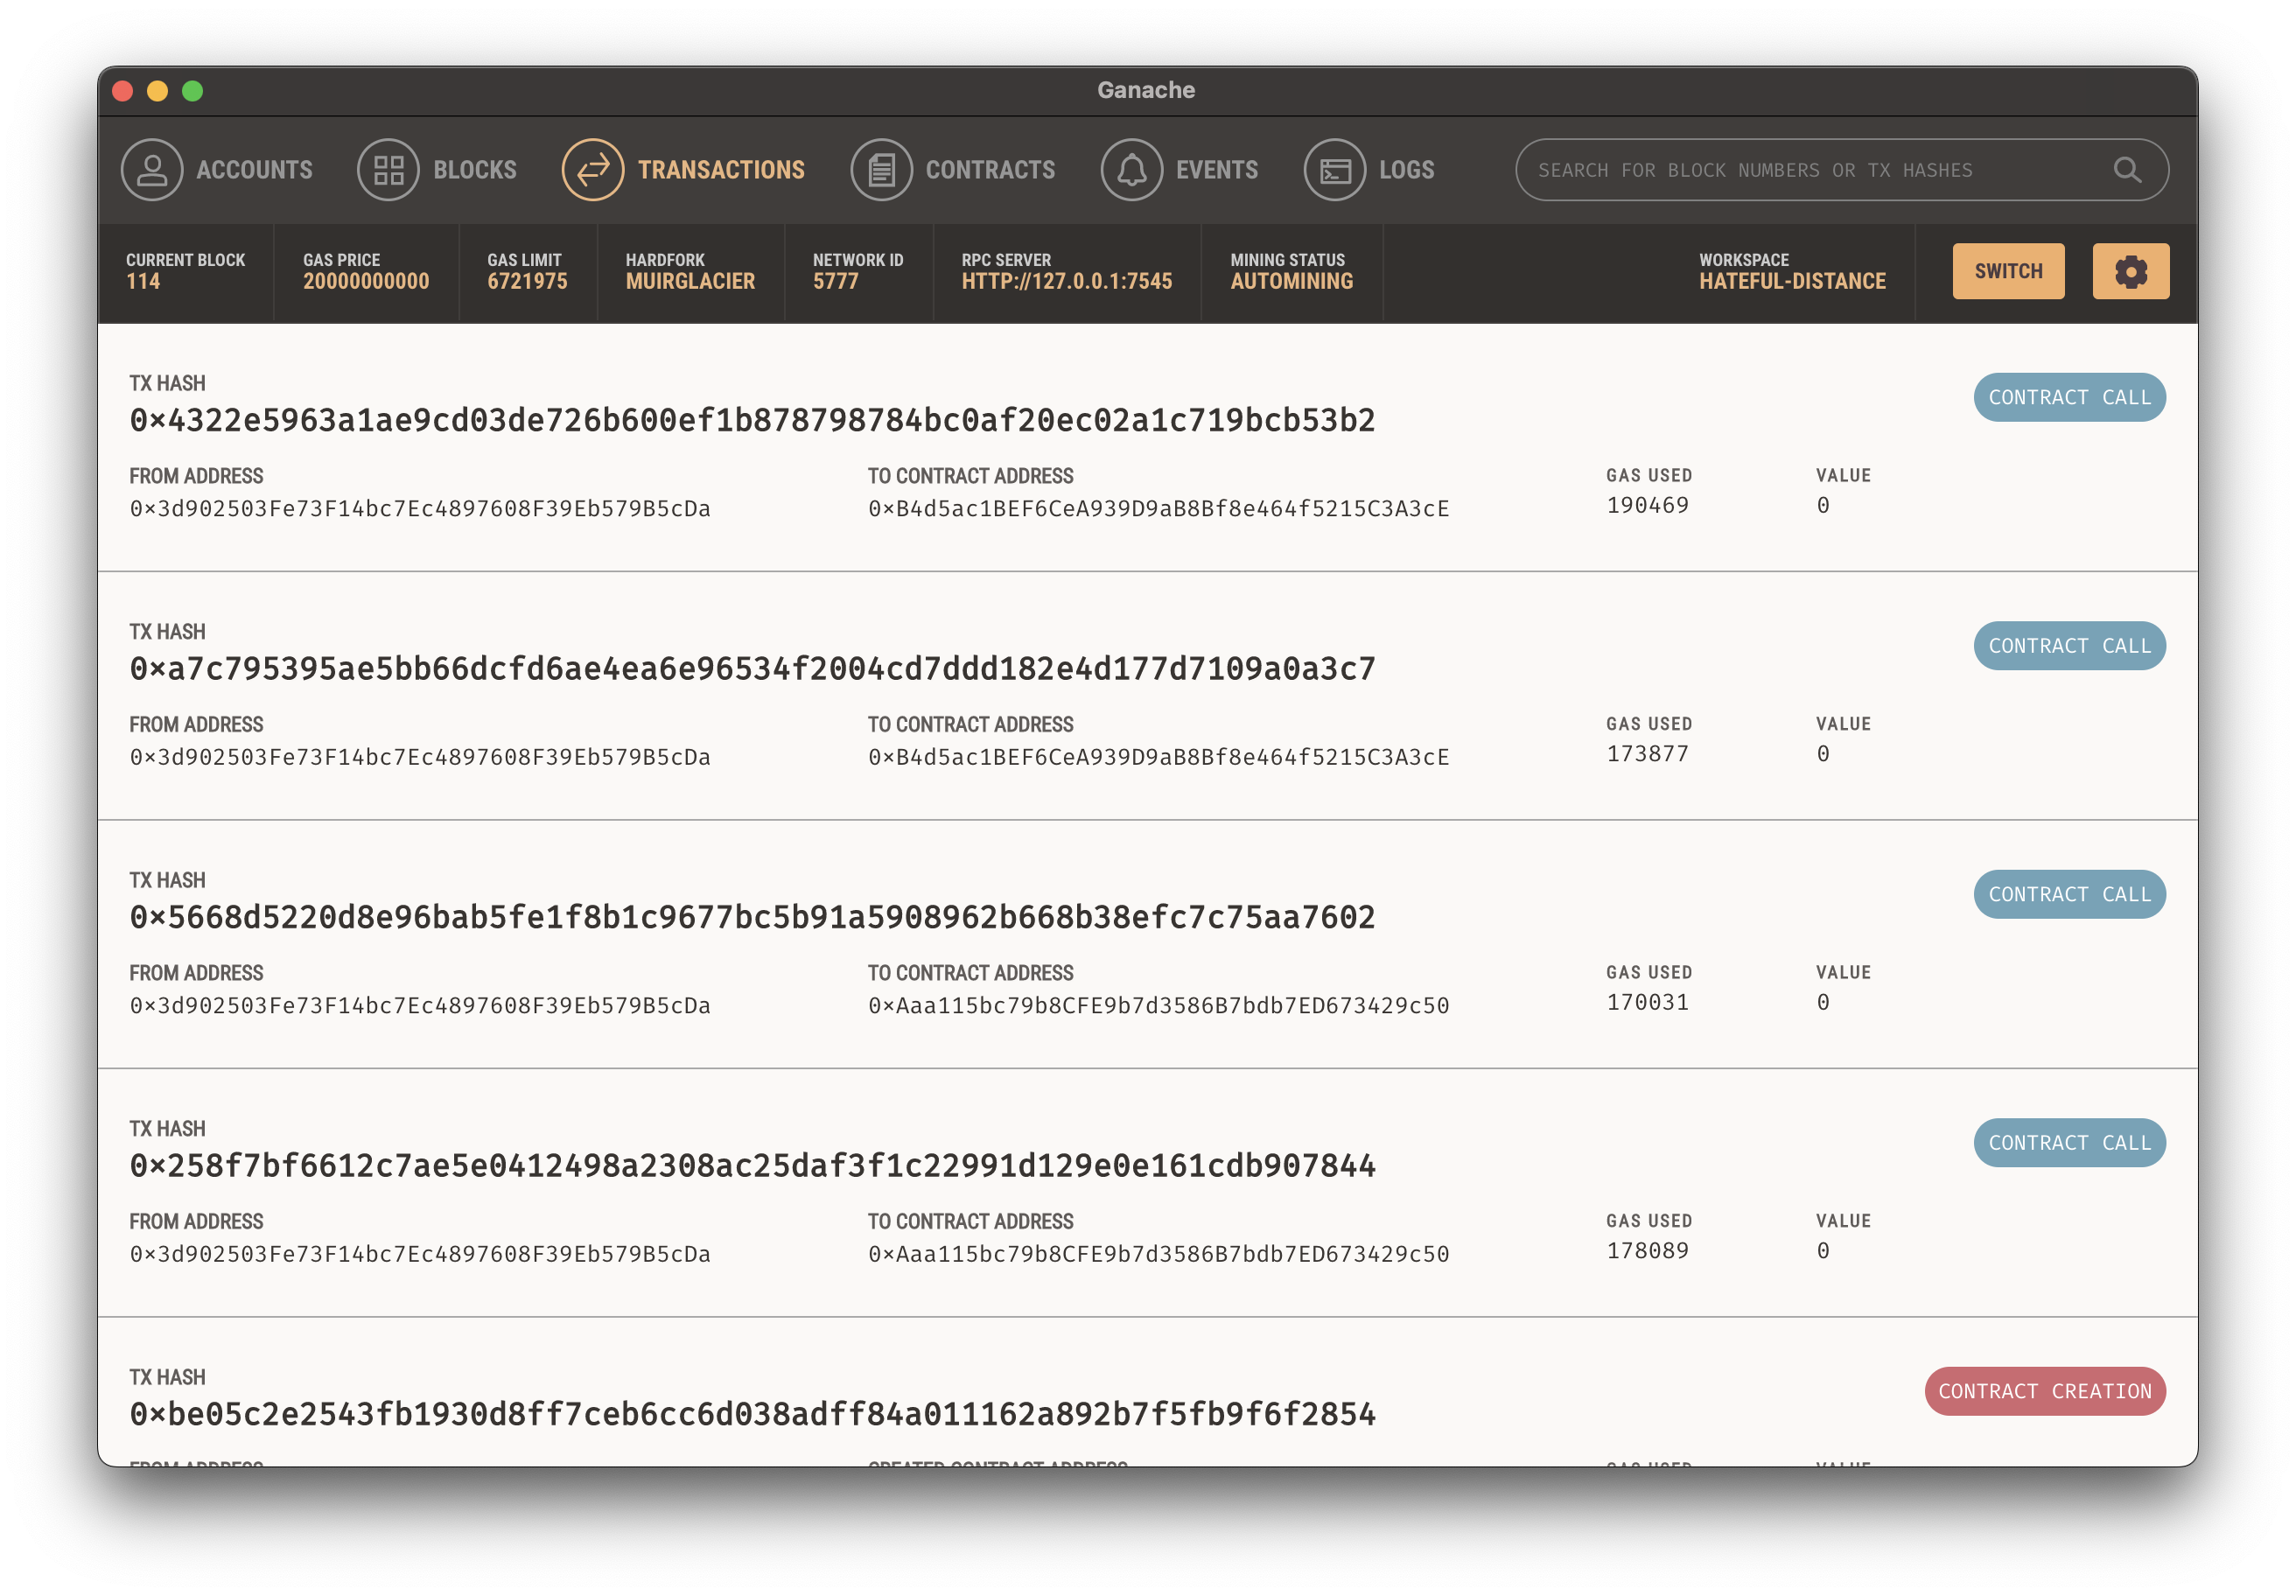
\includegraphics[width=13cm]{media/Ganache_Transactions.png}
\centering
\caption{Ganache Transactions}
\end{figure}
\begin{figure} [H]
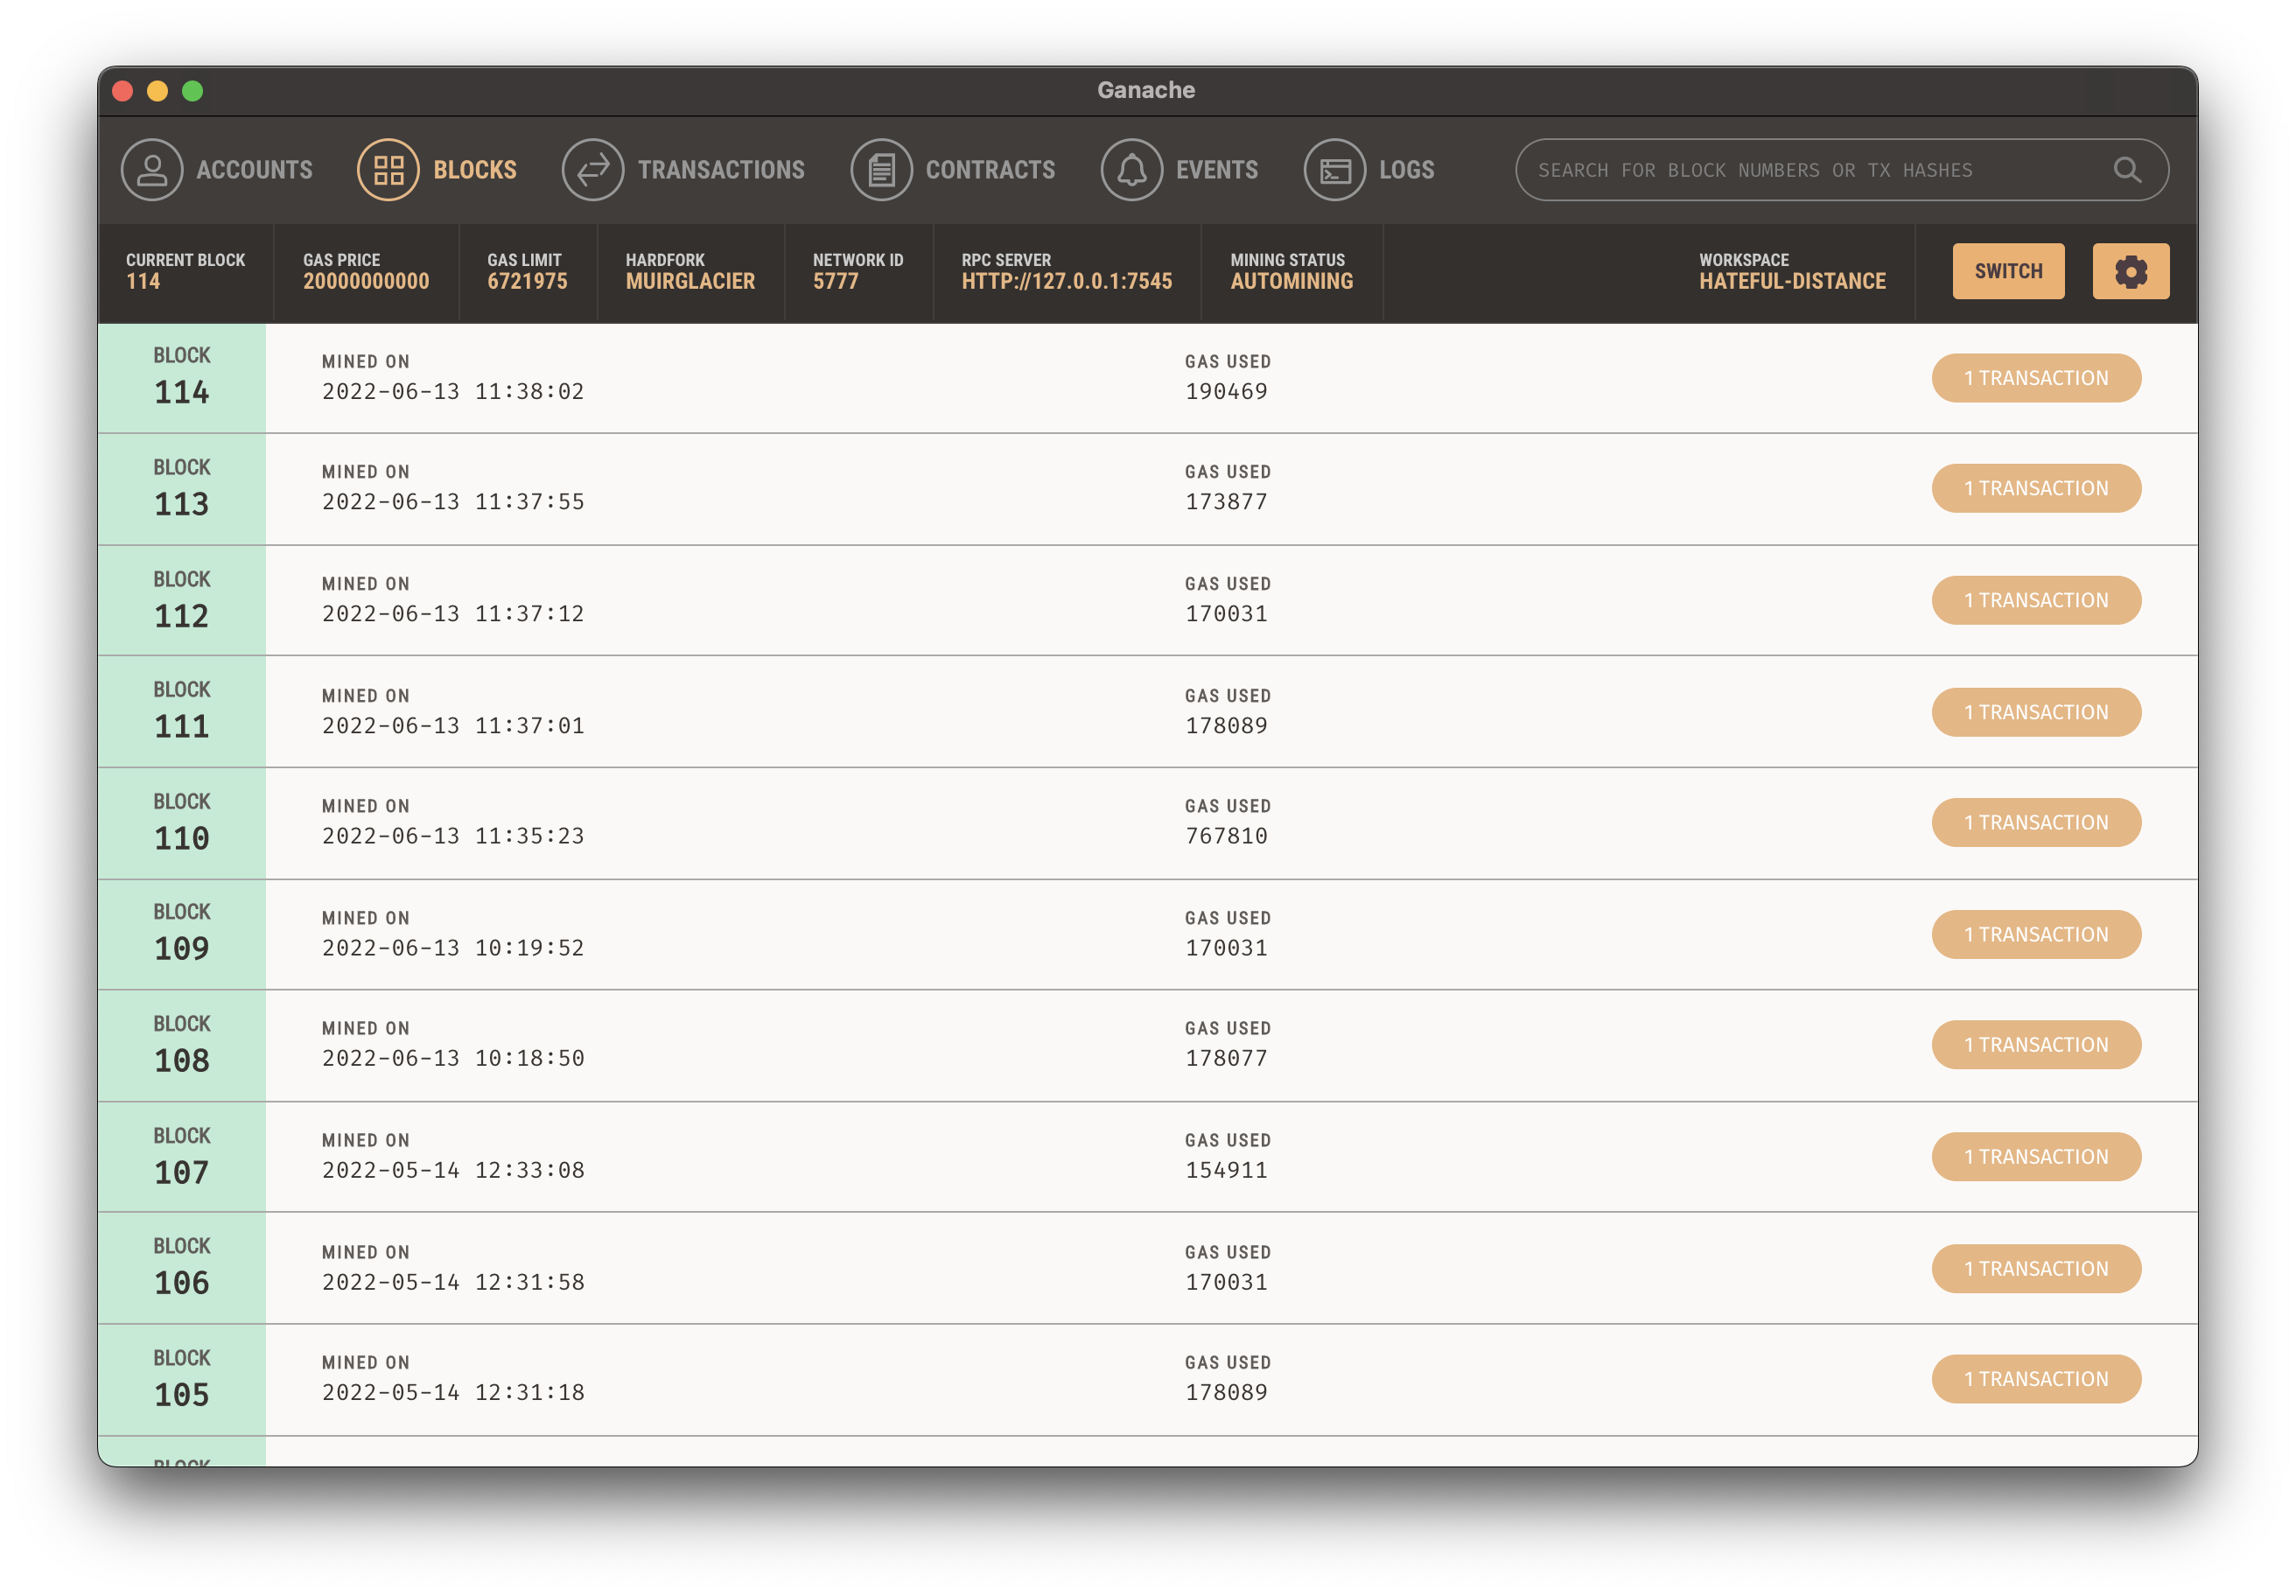
\includegraphics[width=13cm]{media/Ganache_Blocks.png}
\centering
\caption{Ganache Blocks}
\end{figure}
\begin{figure} [H]
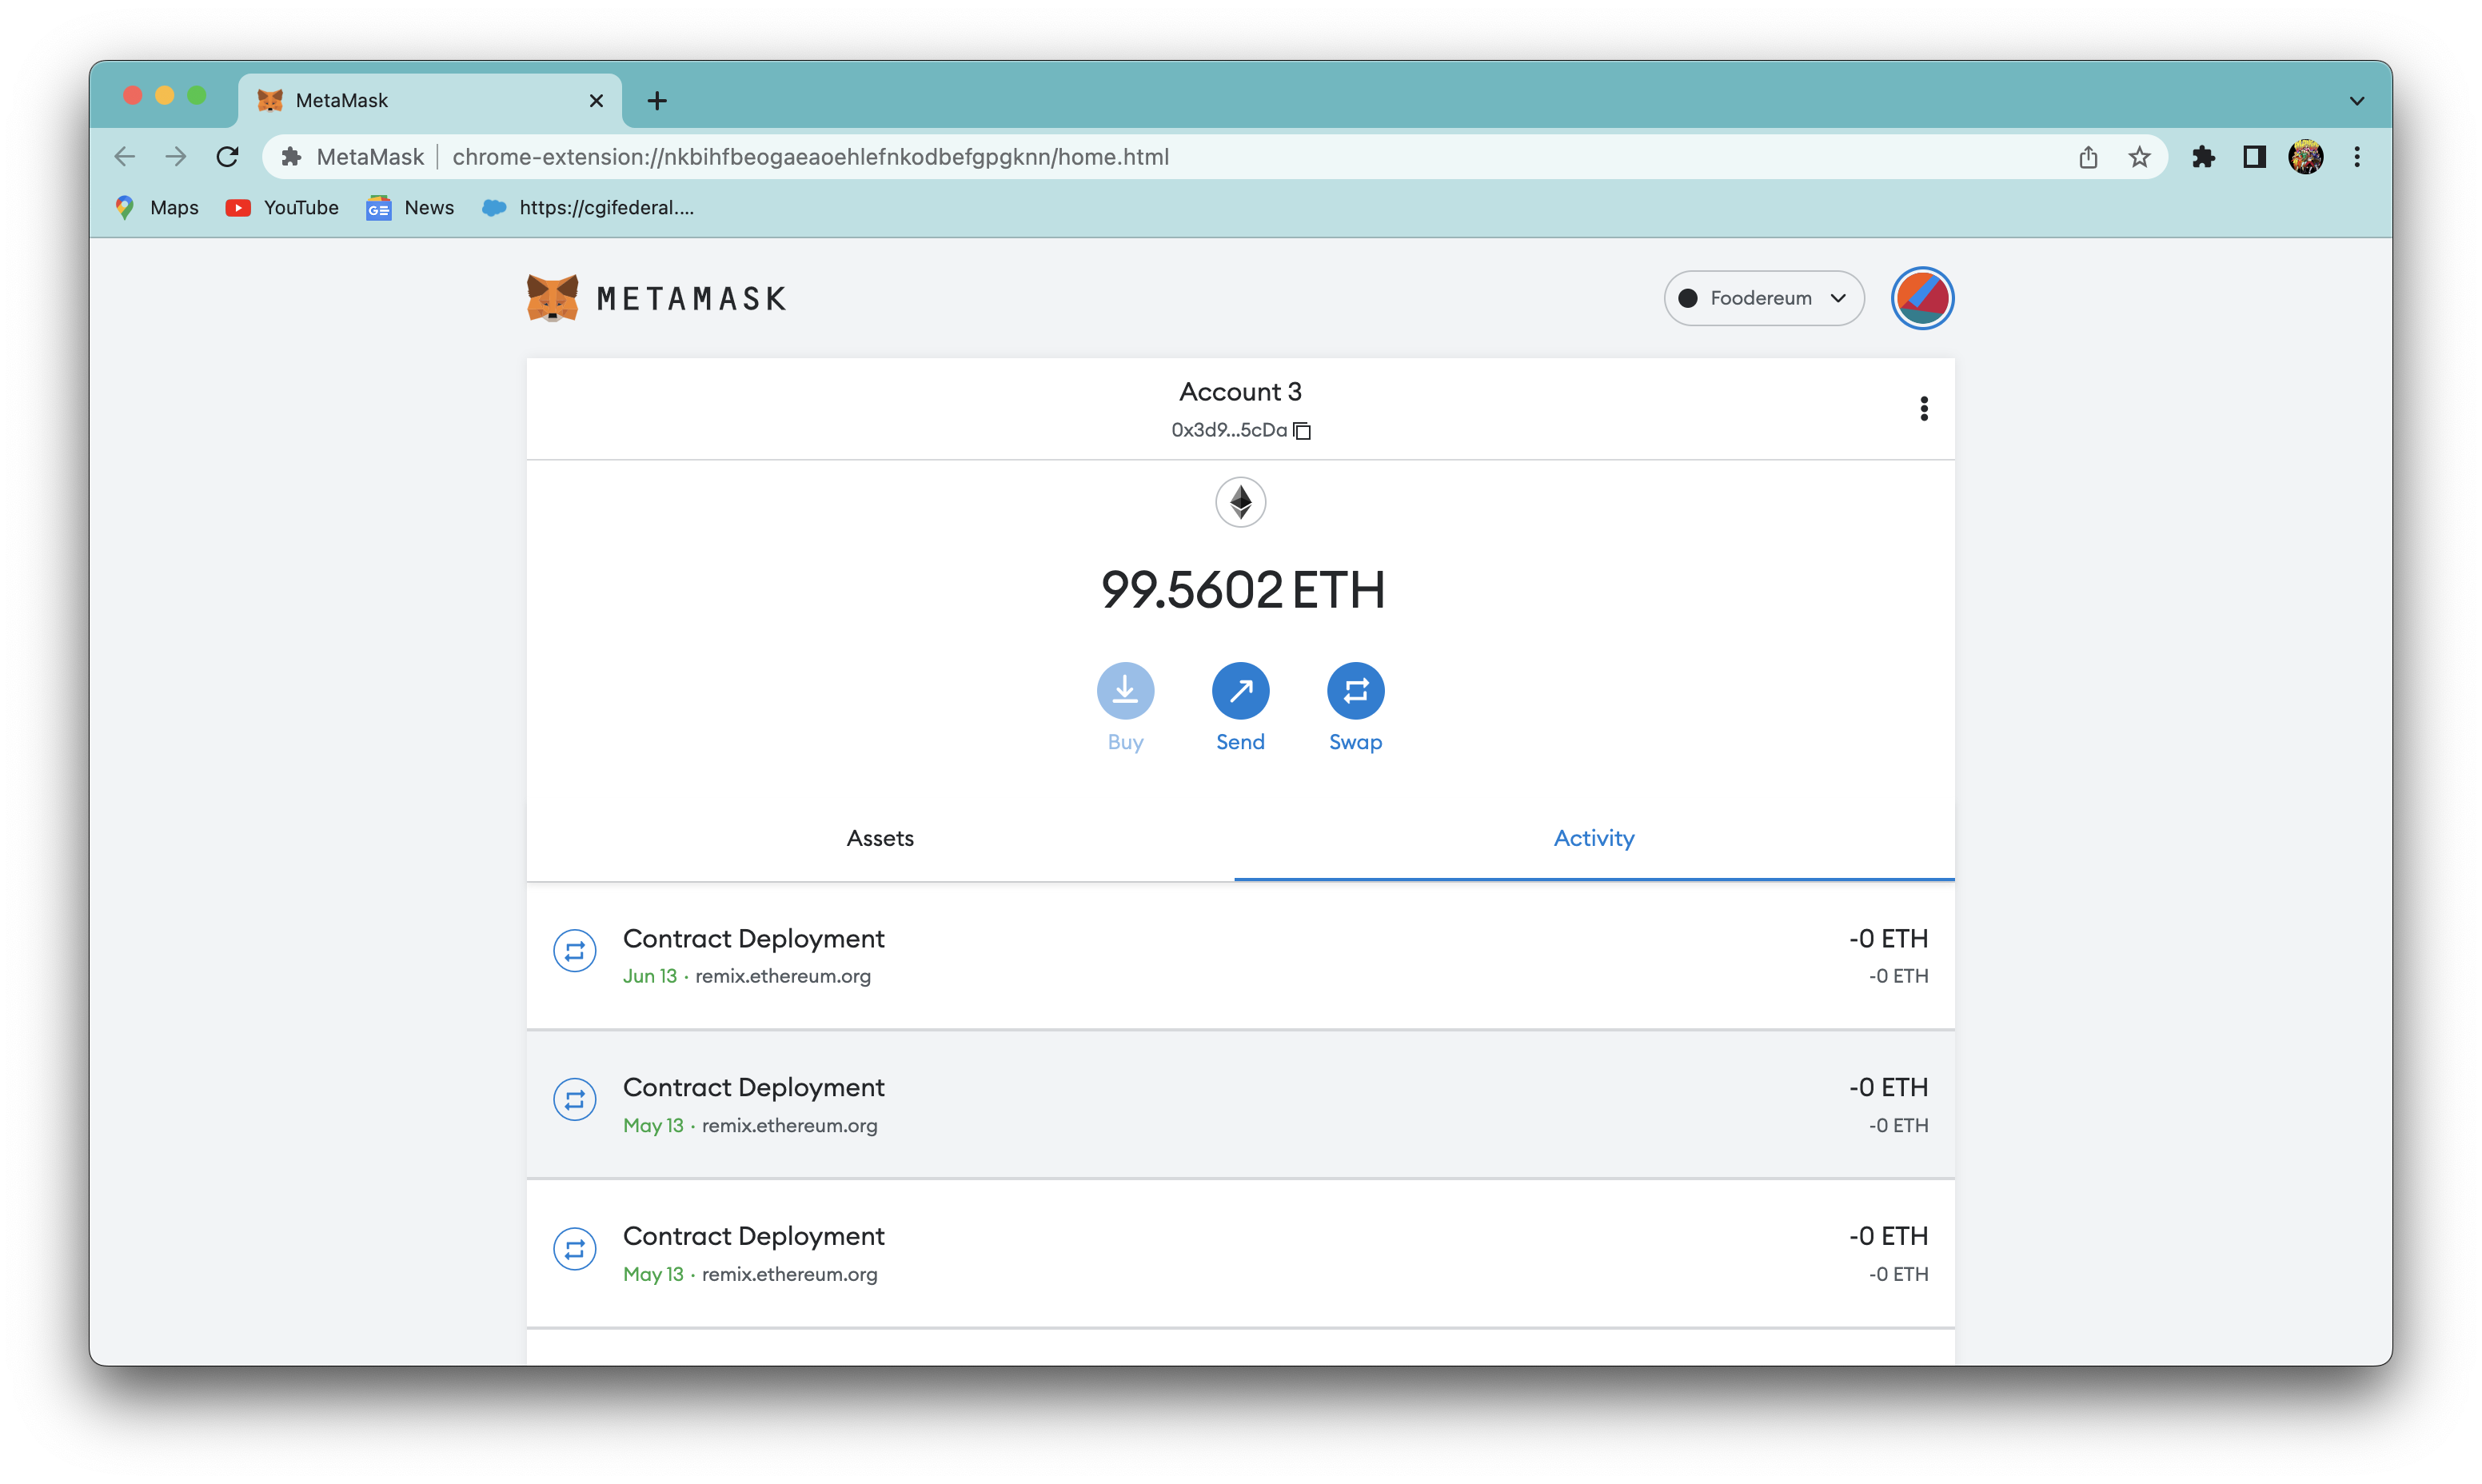
\includegraphics[width=15cm]{media/Metamask_Foodereum.png}
\centering
\caption{Metamask with Personalized Network}
\end{figure}
\begin{figure} [H]
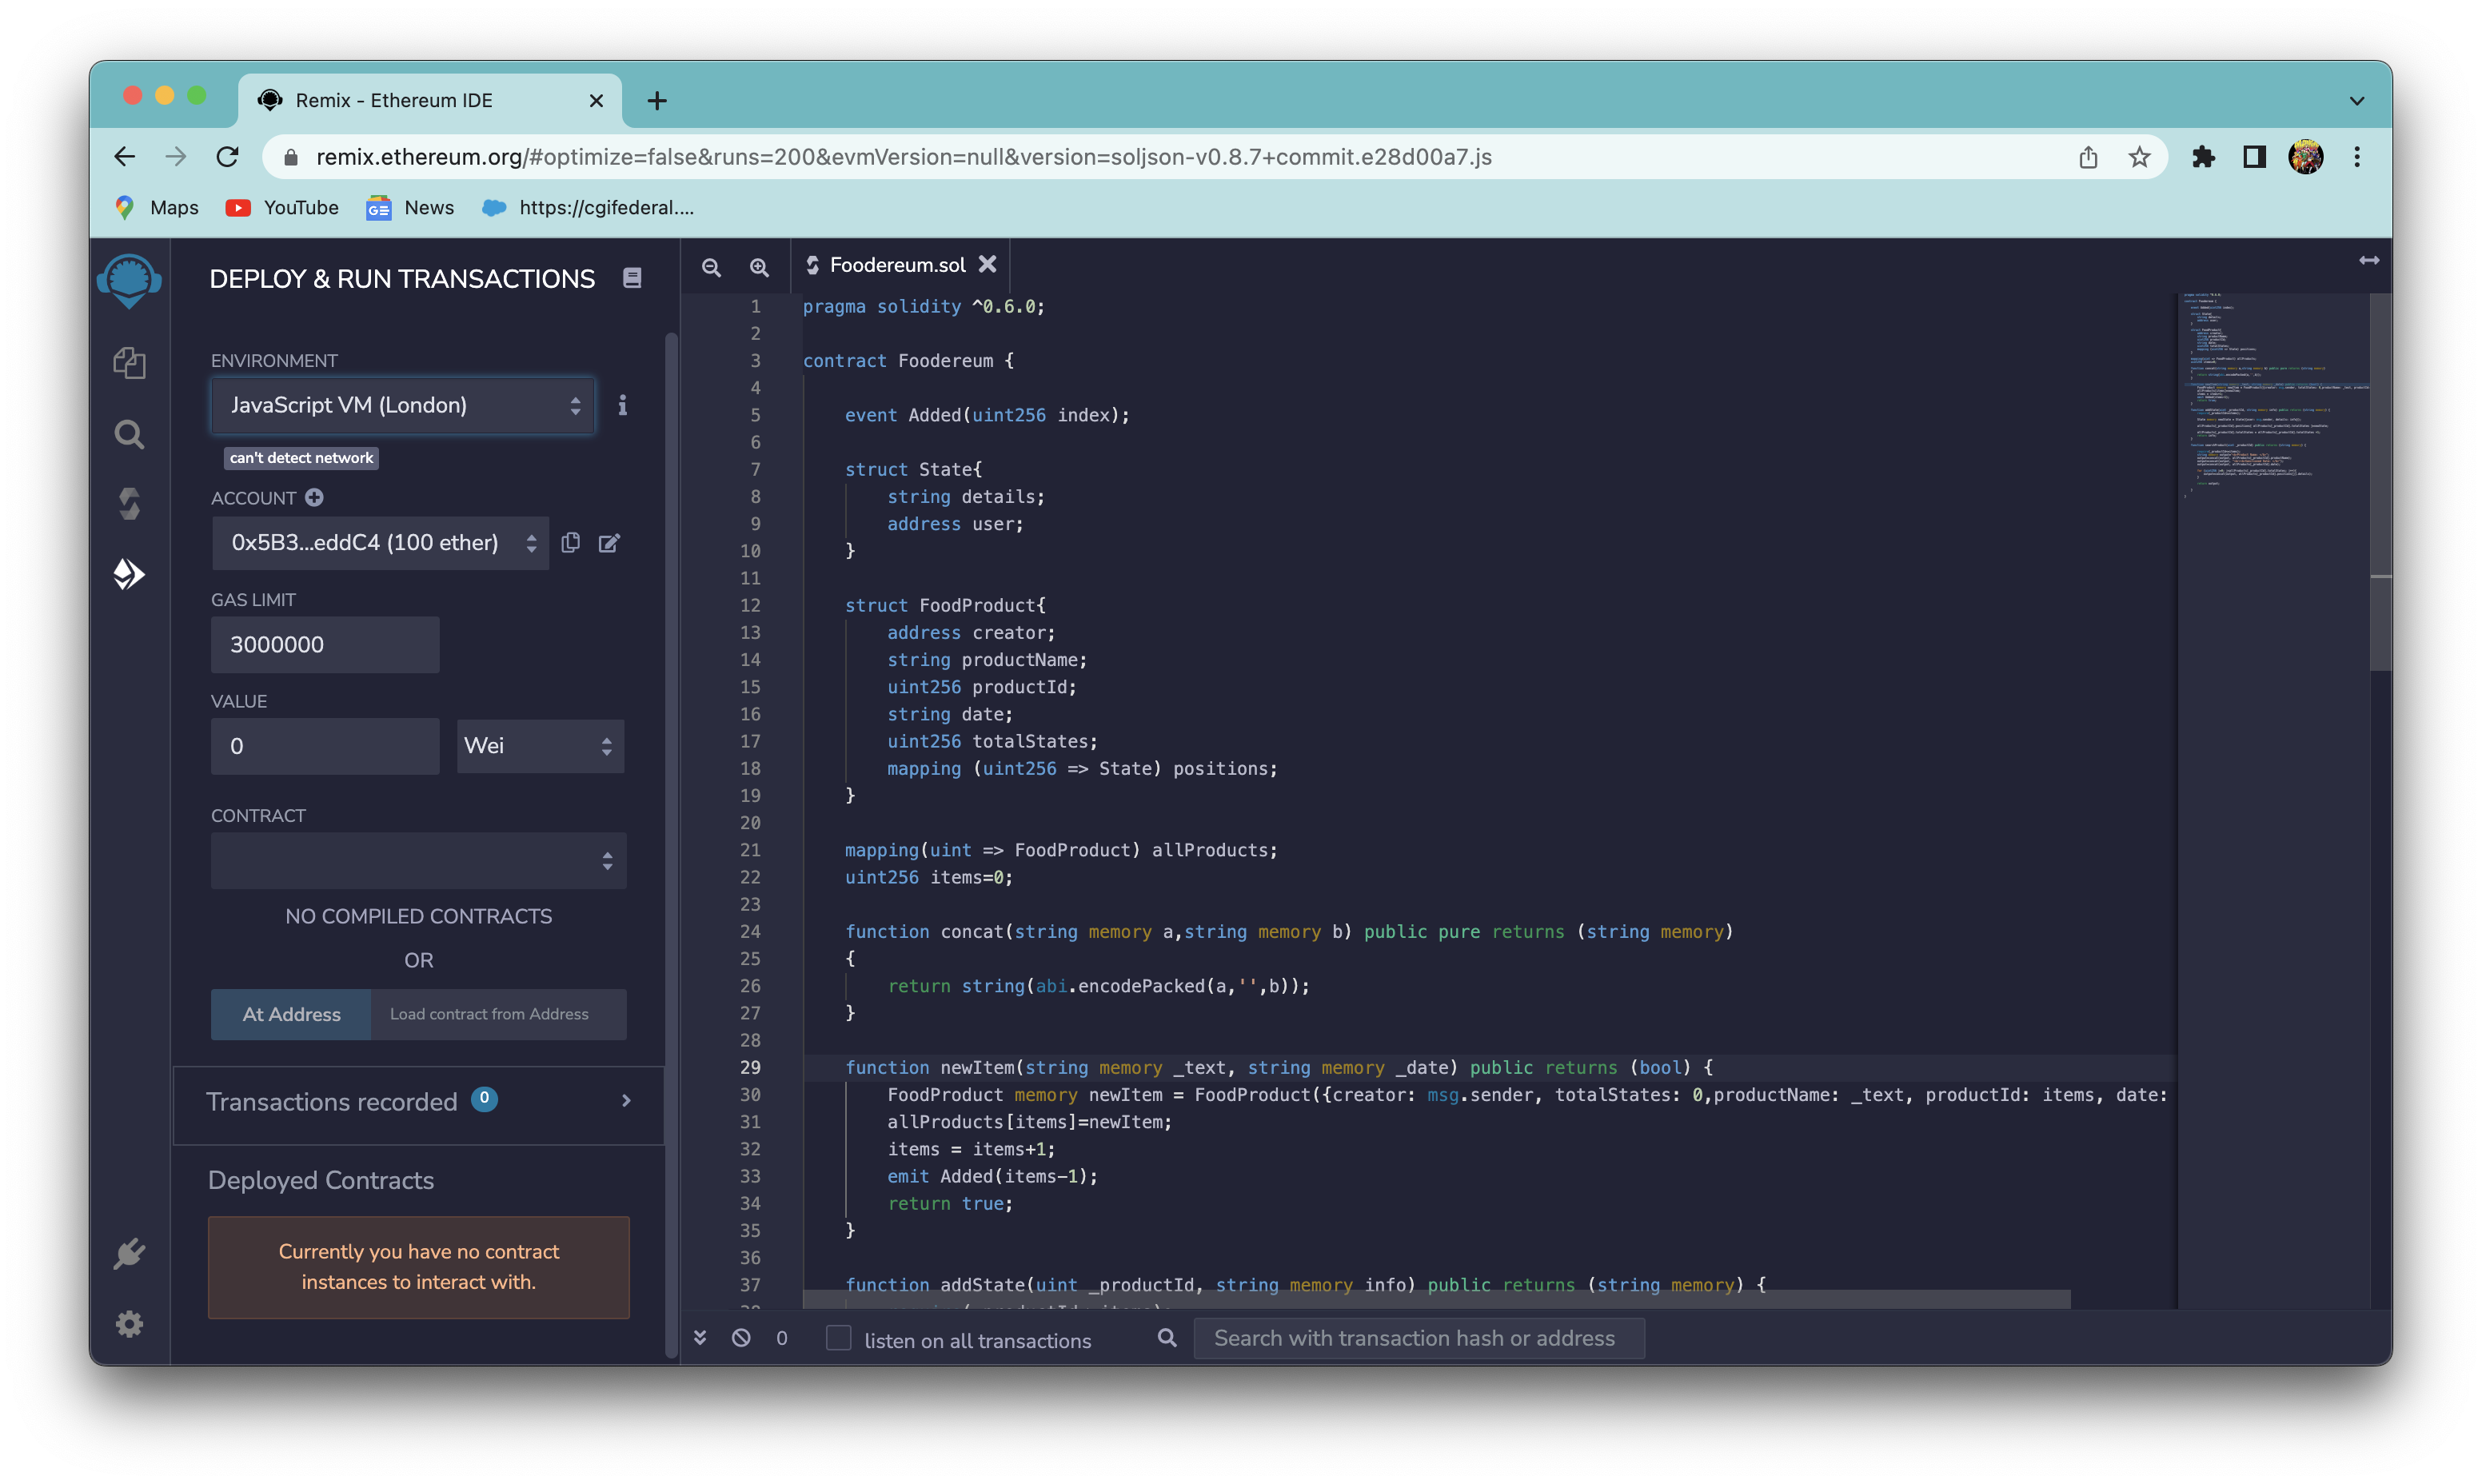
\includegraphics[width=15cm]{media/Remix.png}
\centering
\caption{Remix IDE}
\end{figure}
\begin{figure} [H]
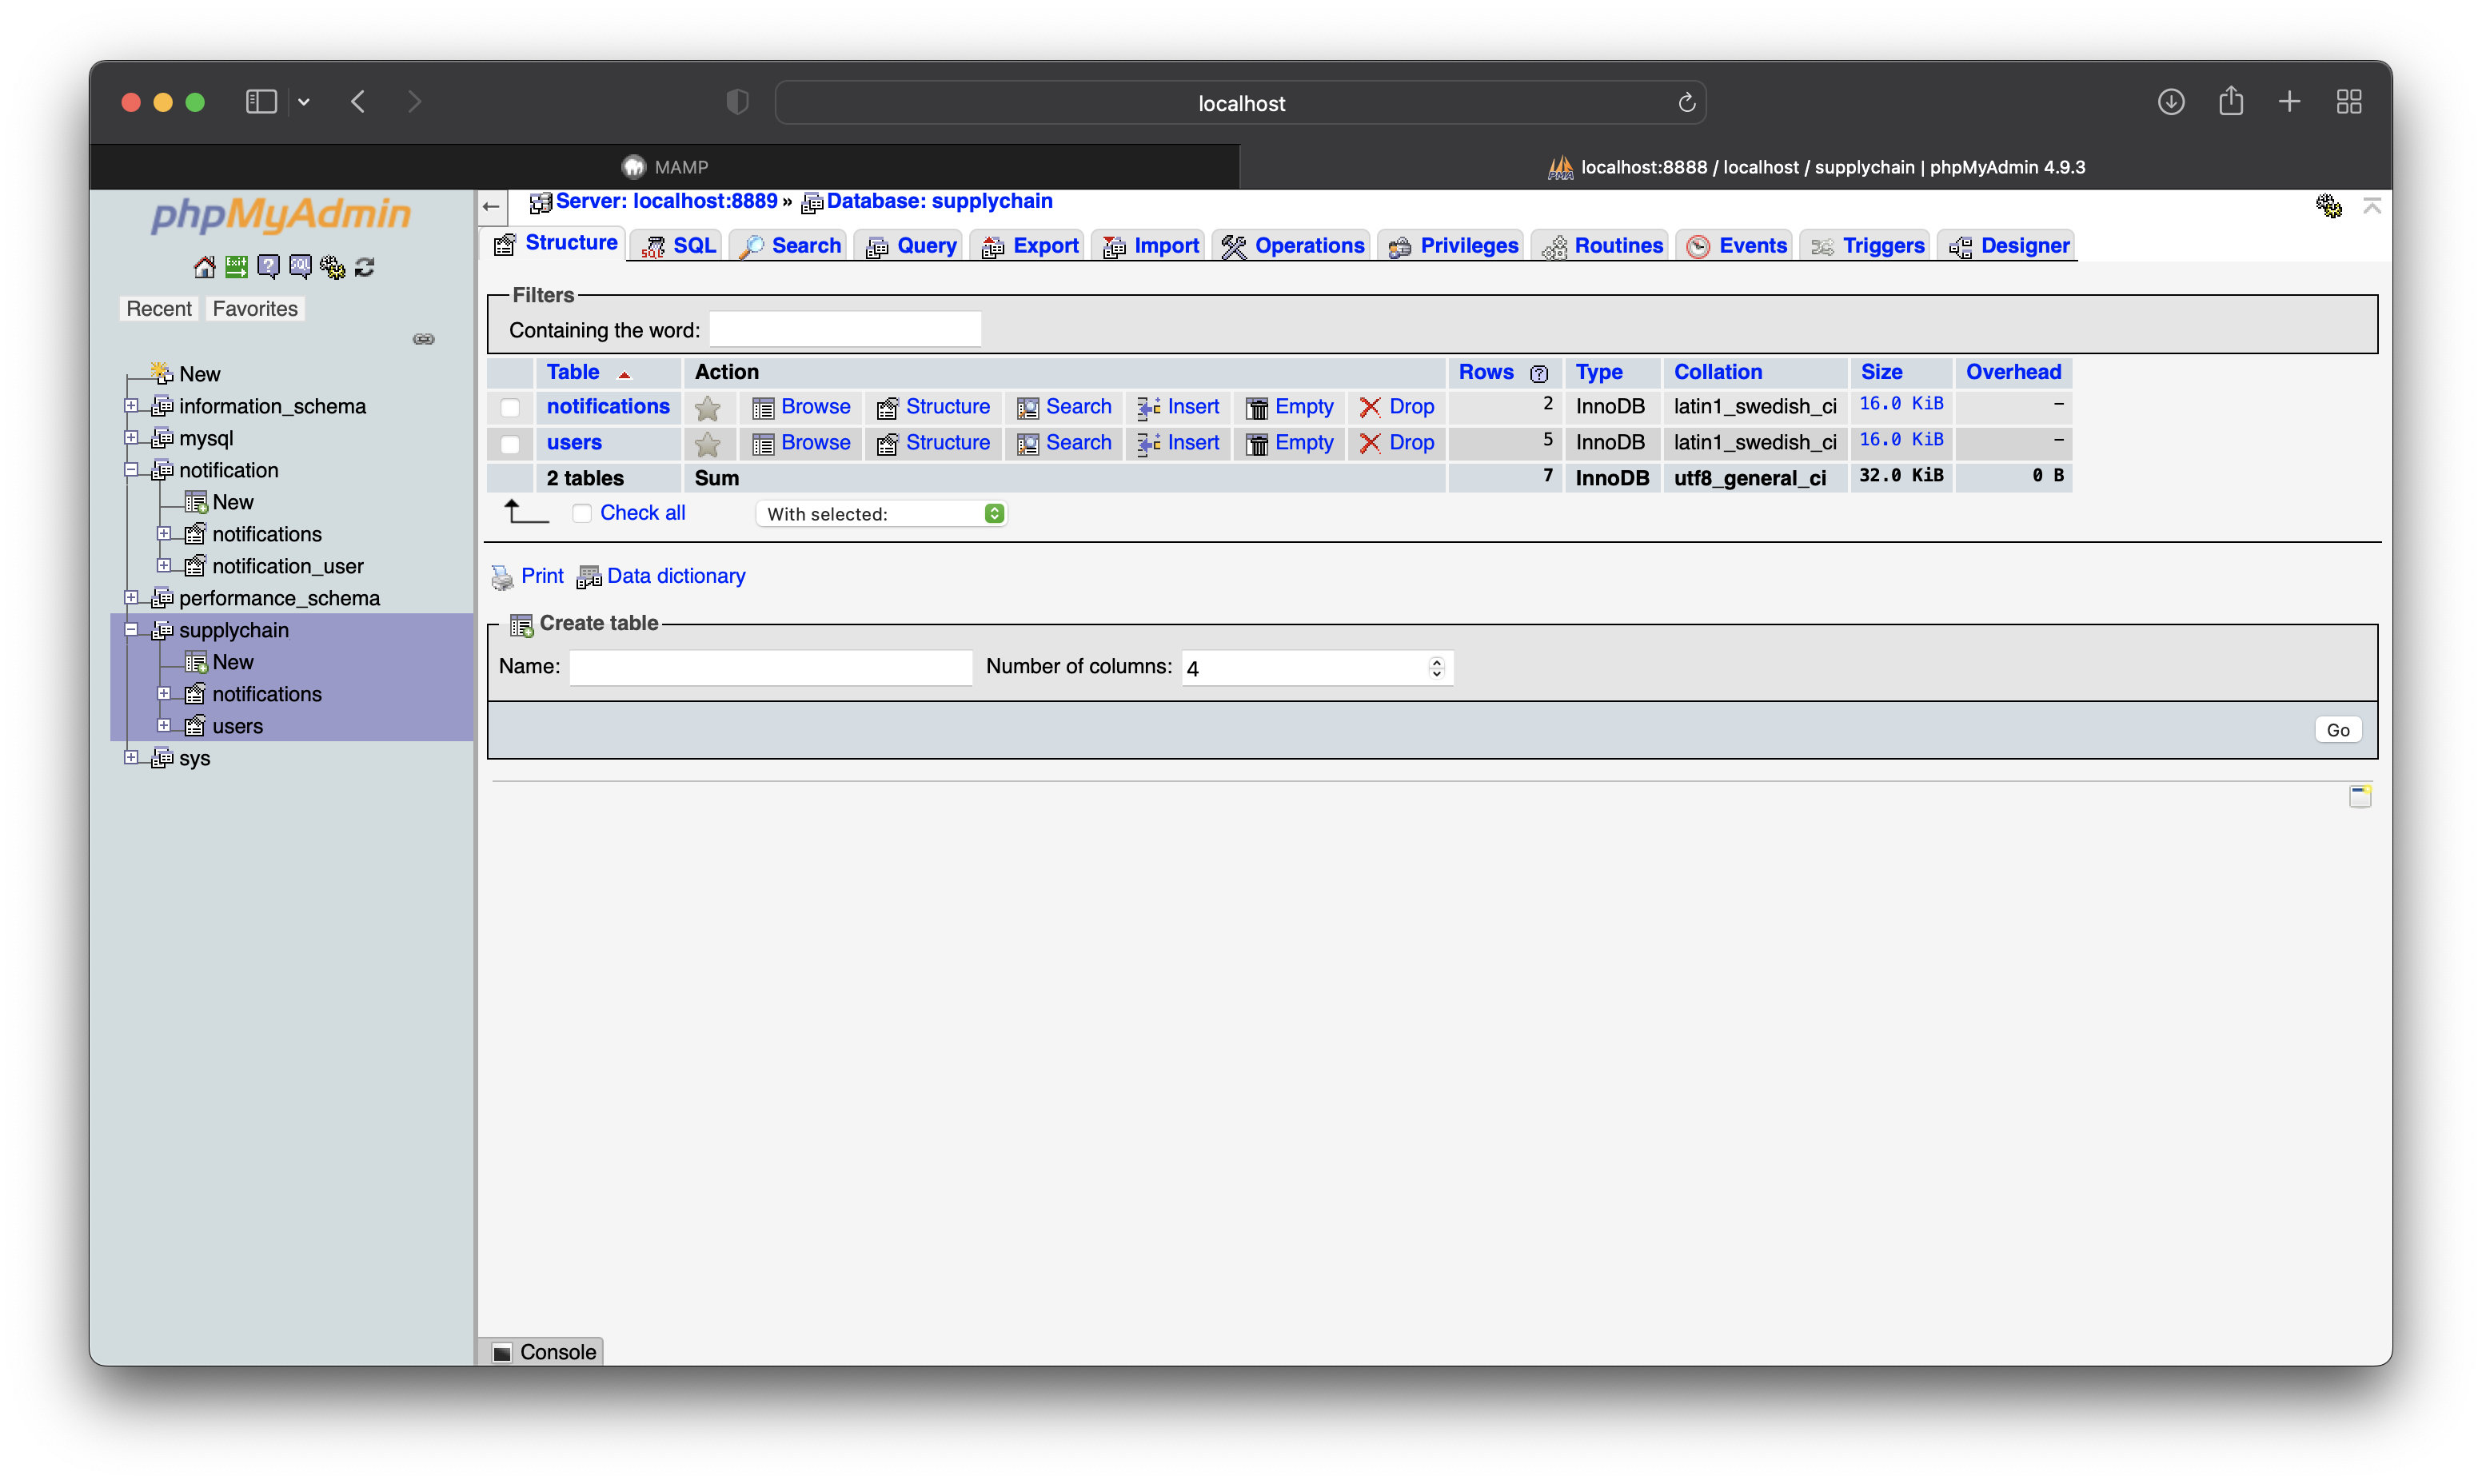
\includegraphics[width=15cm]{media/DBTables.png}
\centering
\caption{MySQL Database Tables}
\end{figure}
\begin{figure} [H]
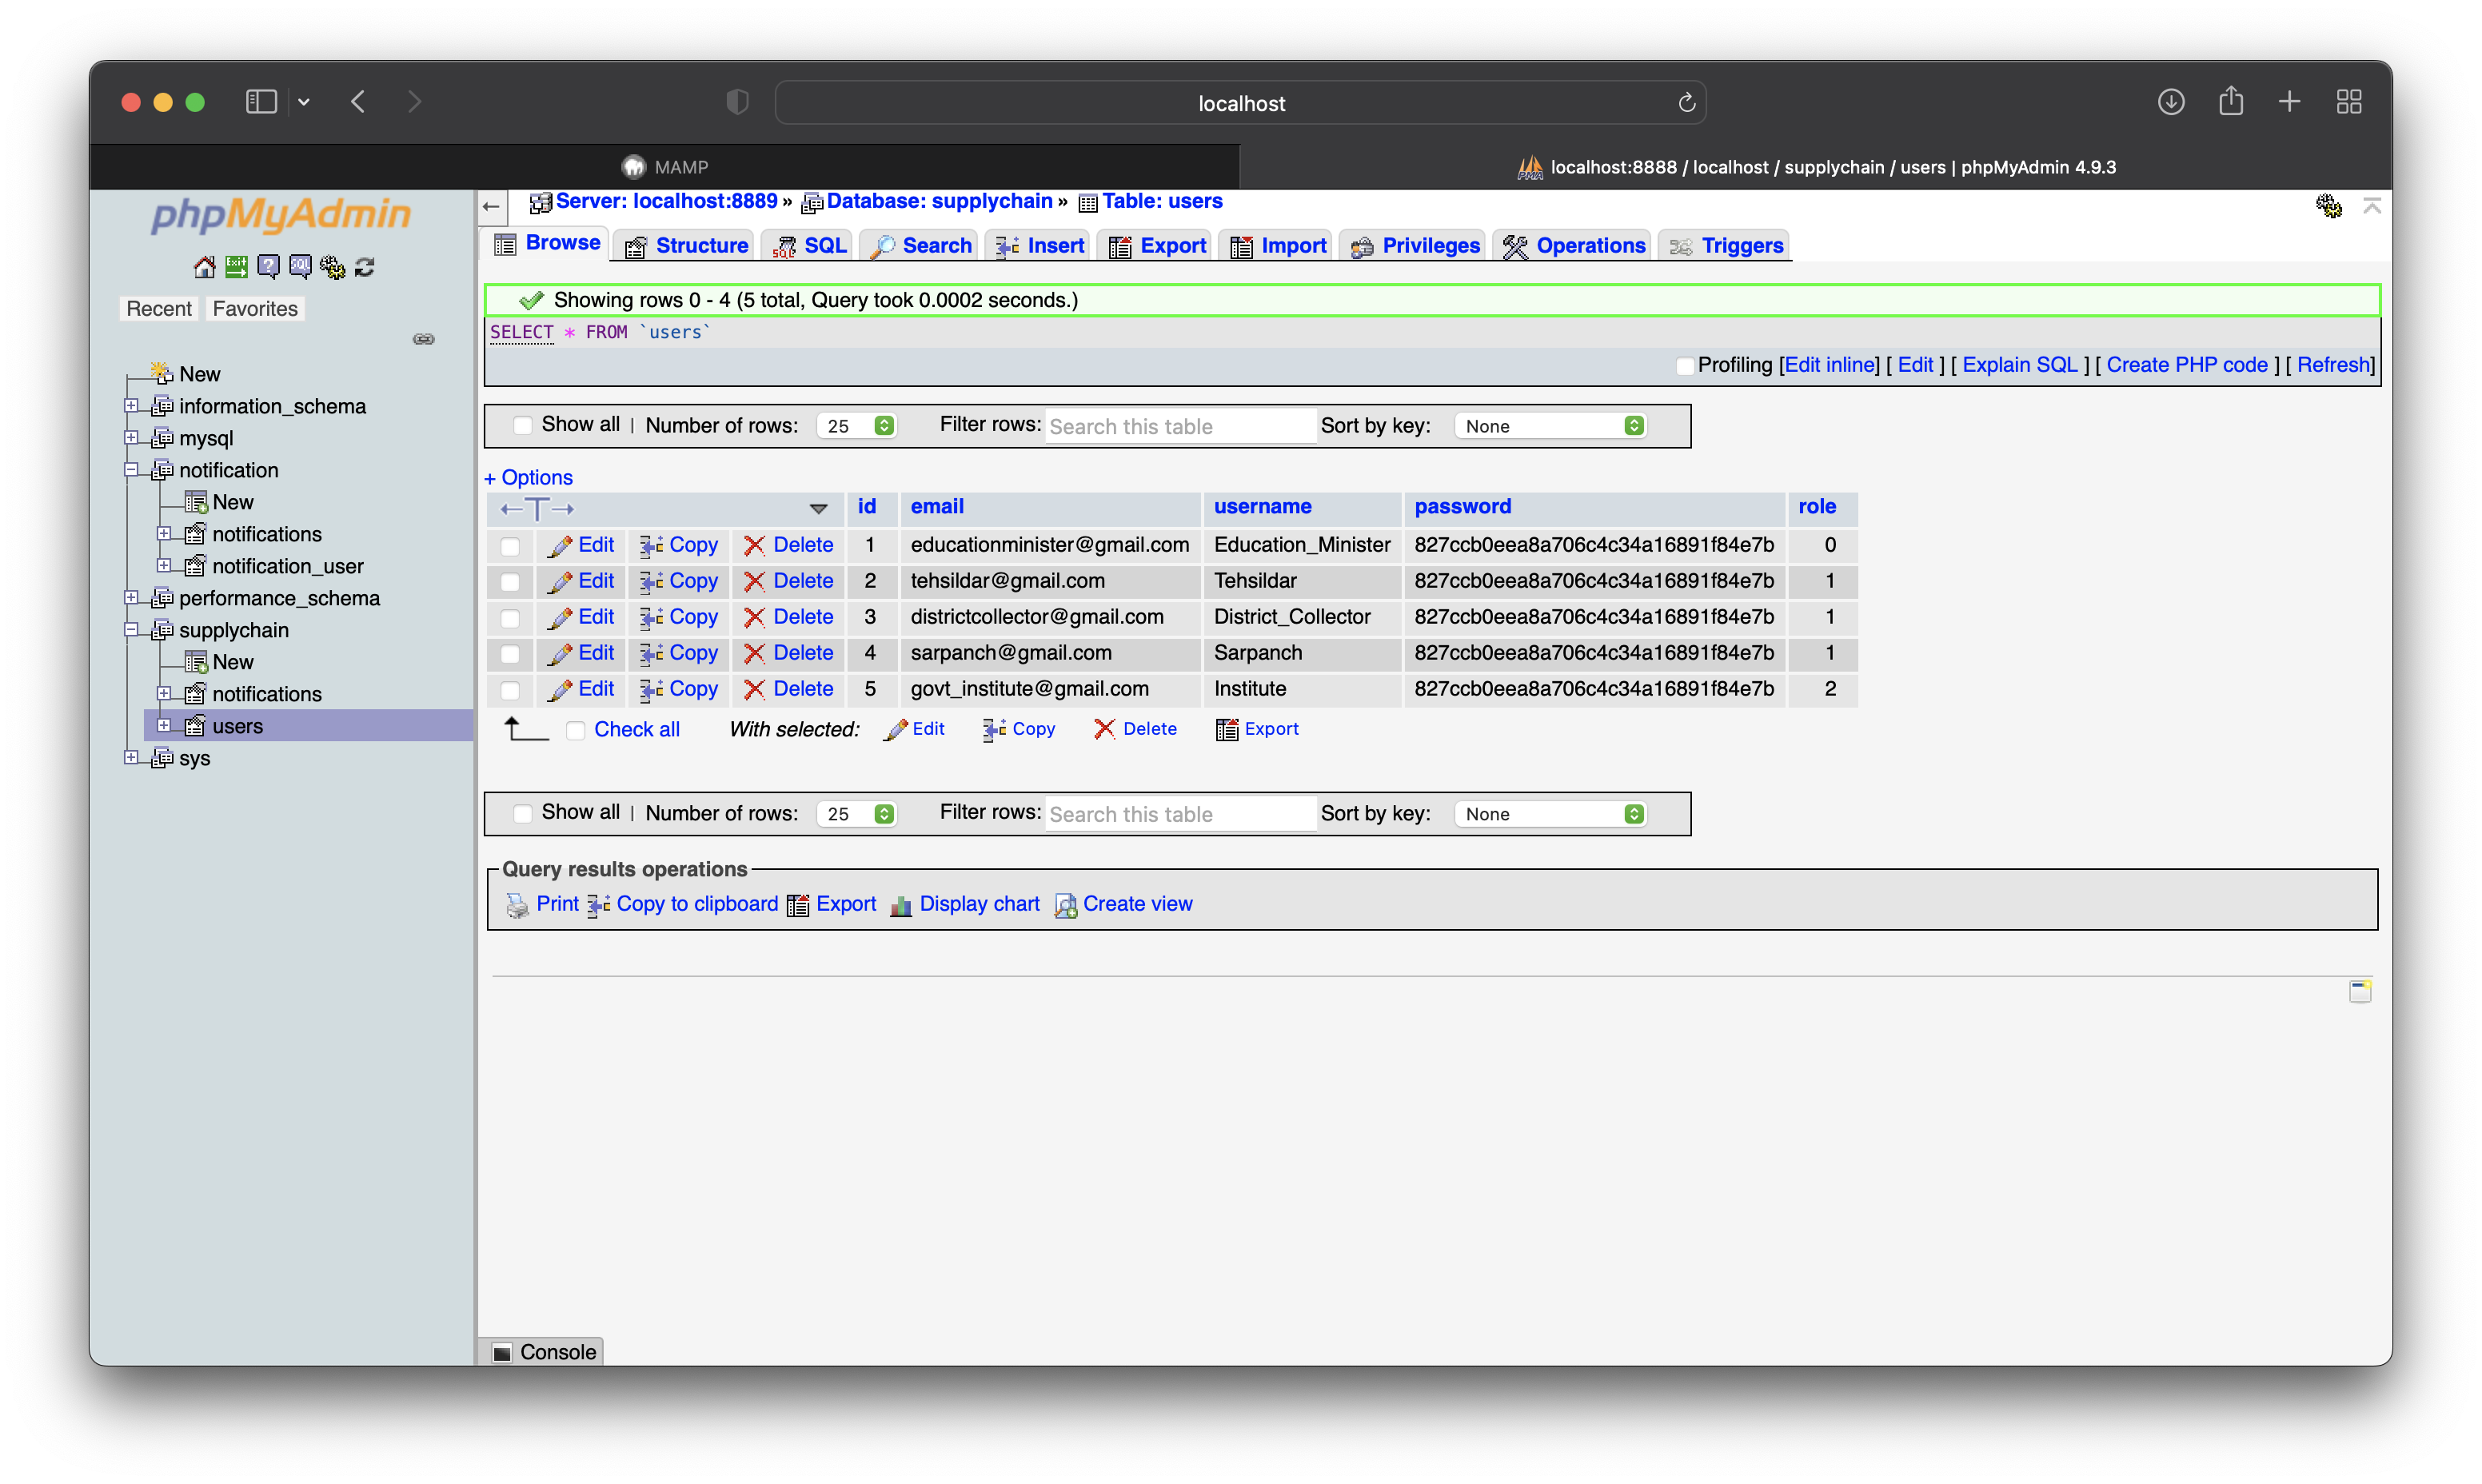
\includegraphics[width=15cm]{media/DBUsers.png}
\centering
\caption{Entities in Supply Chain}
\end{figure}
\newpage
  \pagestyle{fancy}
  \thispagestyle{empty}
  \thispagestyle{plain}
  \fancyhf{}
  \lhead{Foodereum: A Blockchain-based Authenticated Solution for Food Supply Chain $|$}
  \chead{}
  \rhead{Batch No.: 41}
  \renewcommand{\headrulewidth}{0.4pt}%
  \rfoot{Page \thepage \hspace{1pt} of \pageref{LastPage}}
  \lfoot{Dept. of CSE, DSCE}
\renewcommand{\footrulewidth}{0.4pt}%
\renewcommand{\footrulewidth}{0.4pt}% 
\normalsize
\section{Chapter 6: Results} 
\begin{figure} [H]
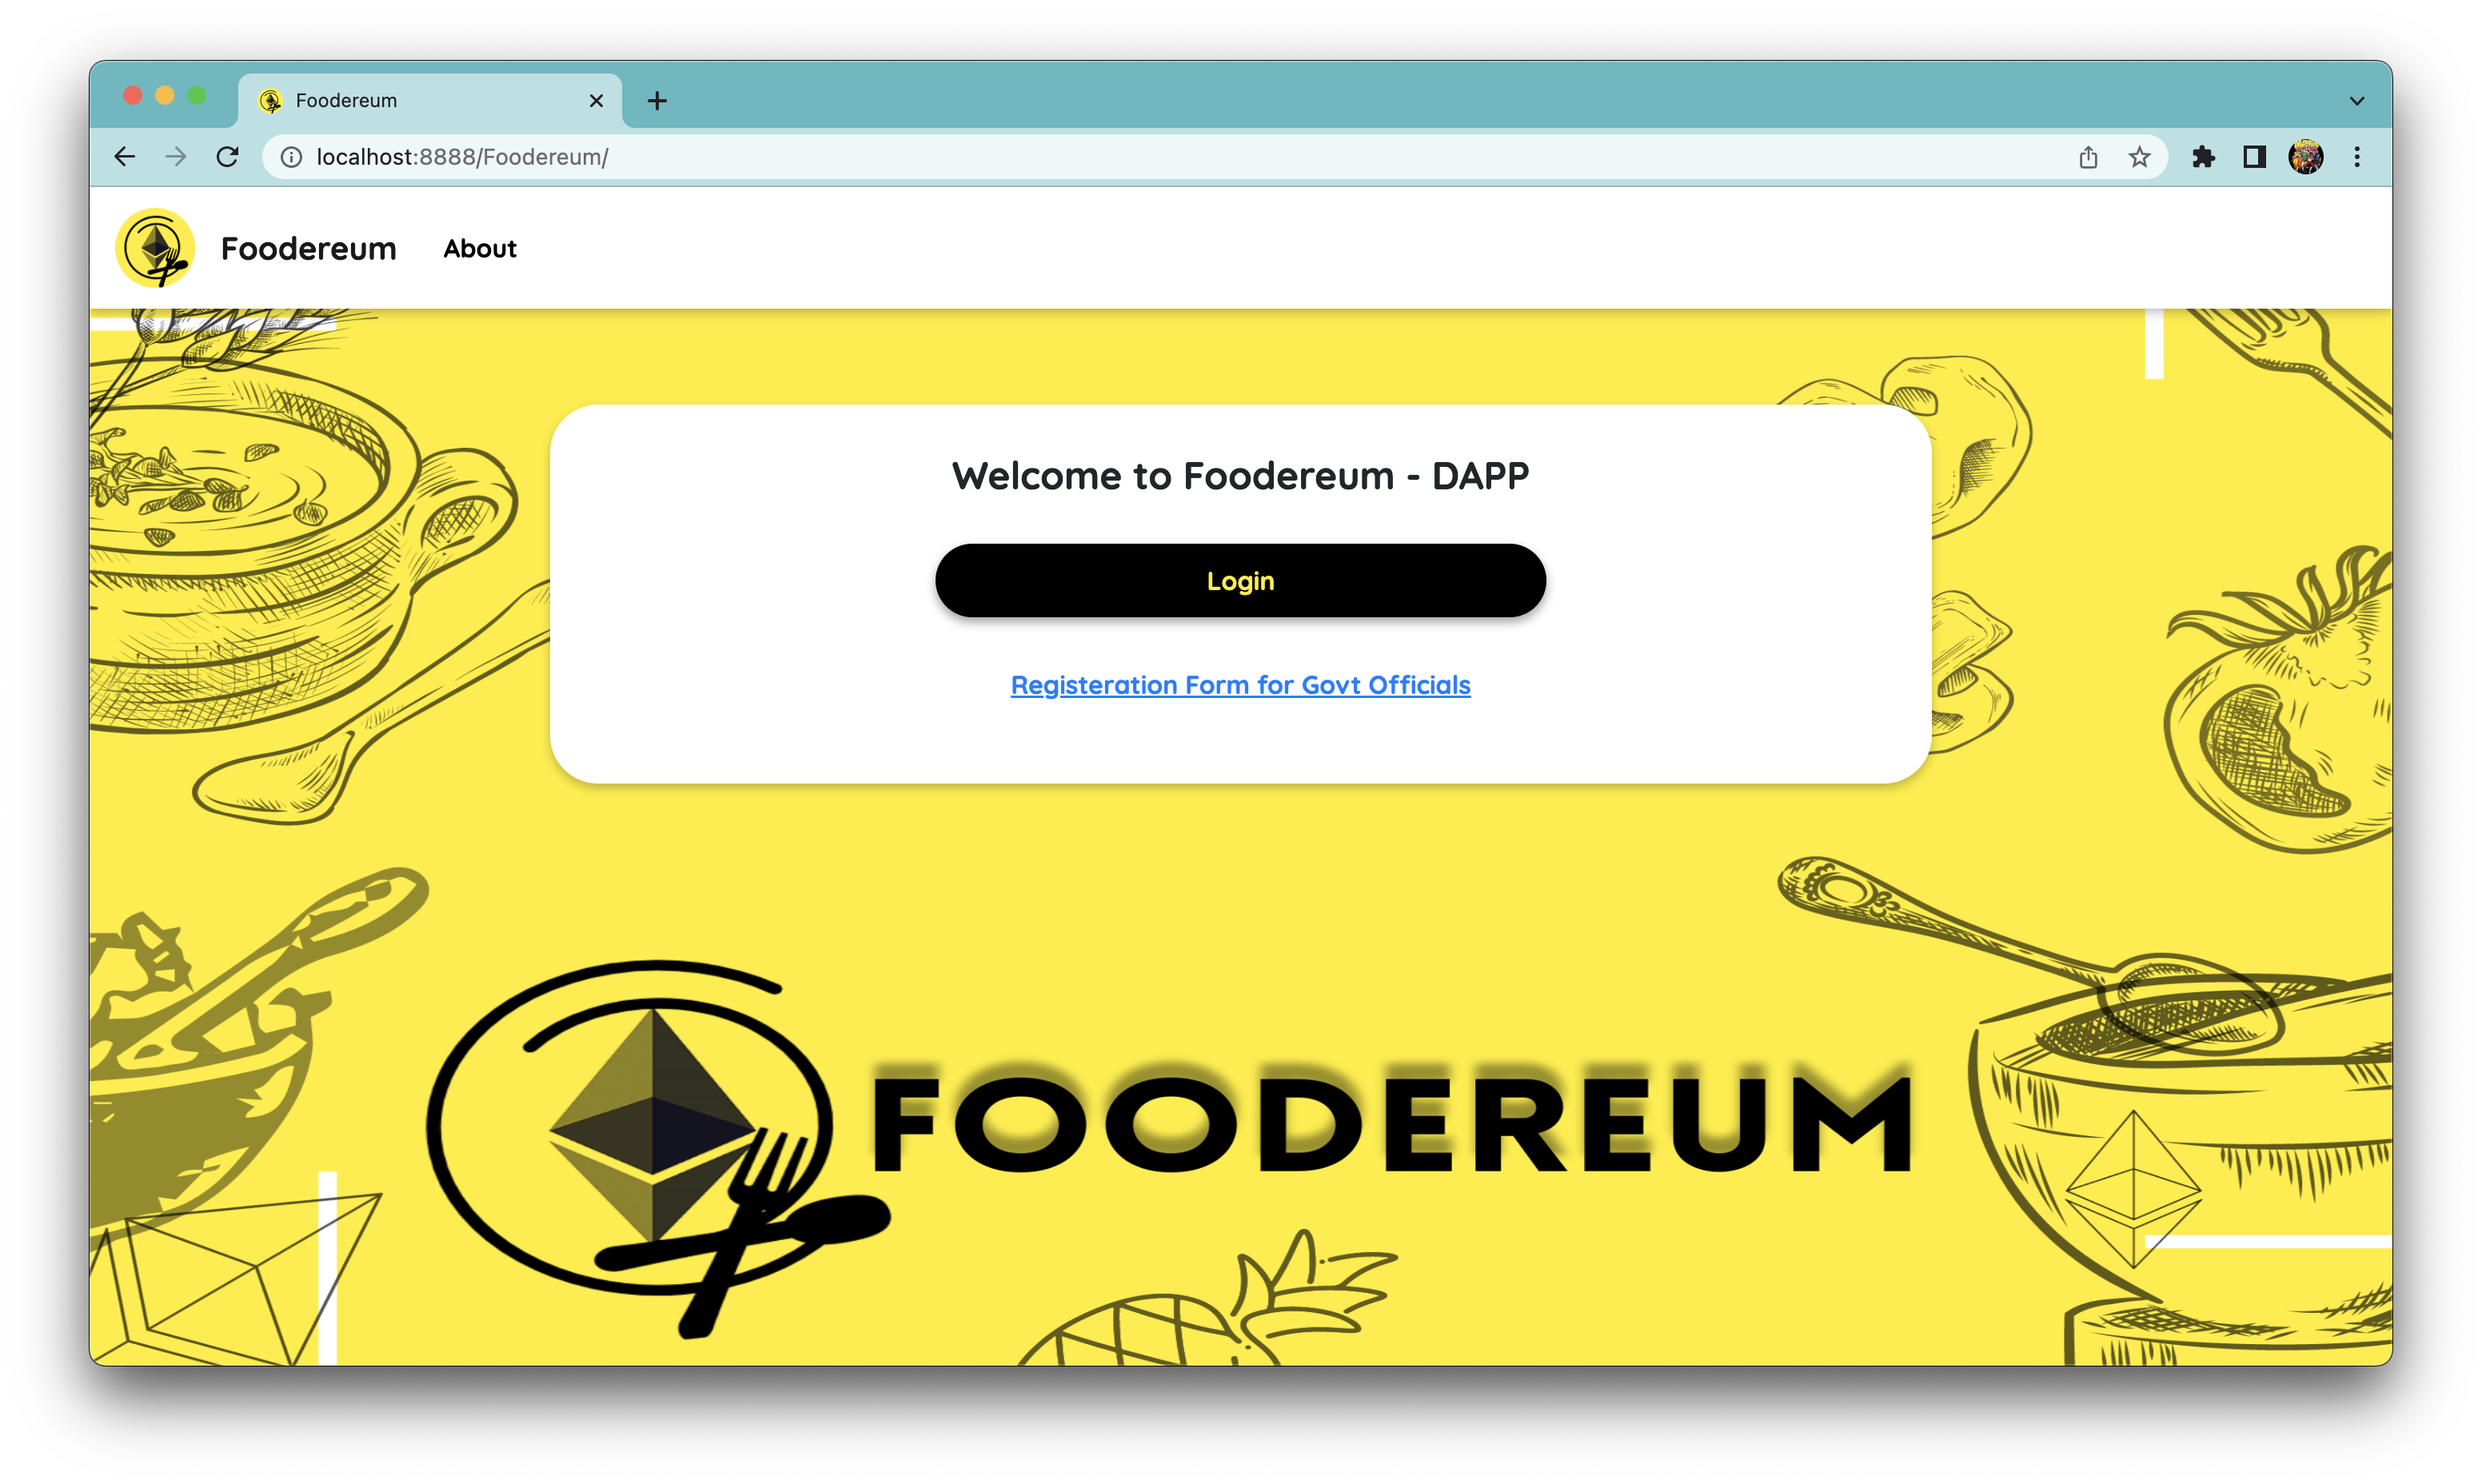
\includegraphics[width=15cm]{media/Login_Page.png}
\centering
\caption{Login Page}
\end{figure}
\begin{figure} [H]
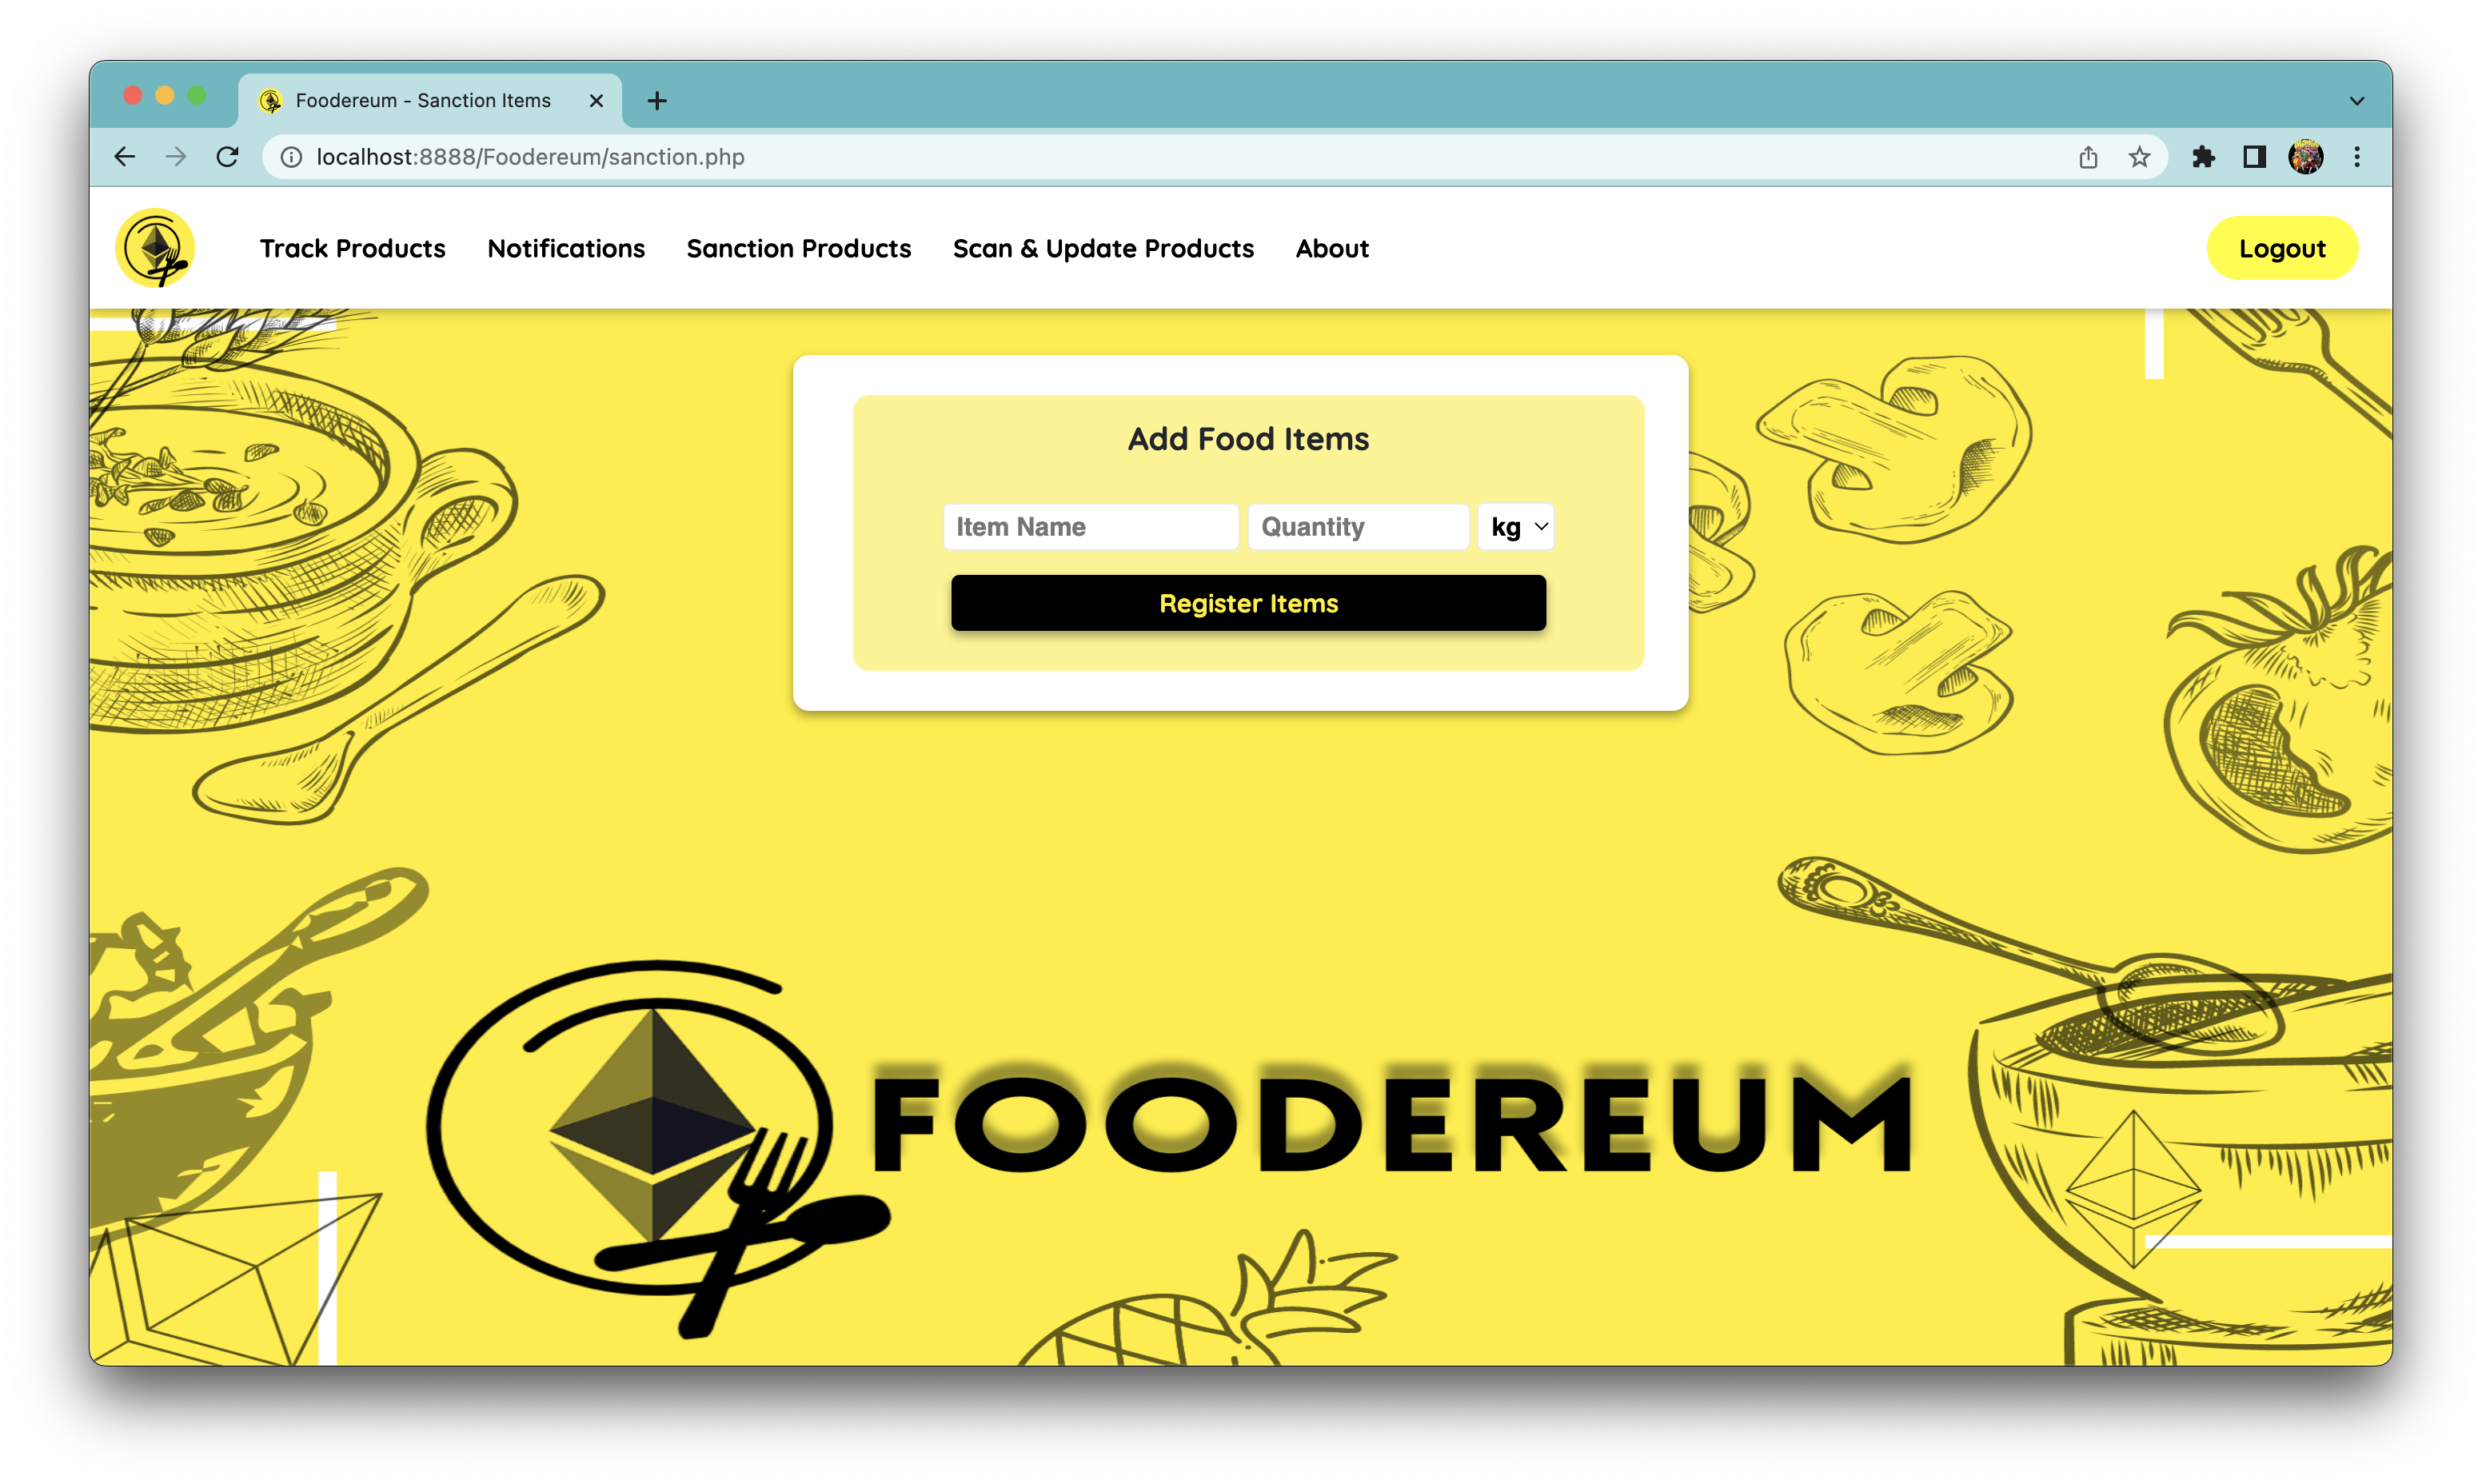
\includegraphics[width=15cm]{media/Sanction_Product.png}
\centering
\caption{Sanction Products Page}
\end{figure}
\begin{figure} [H]
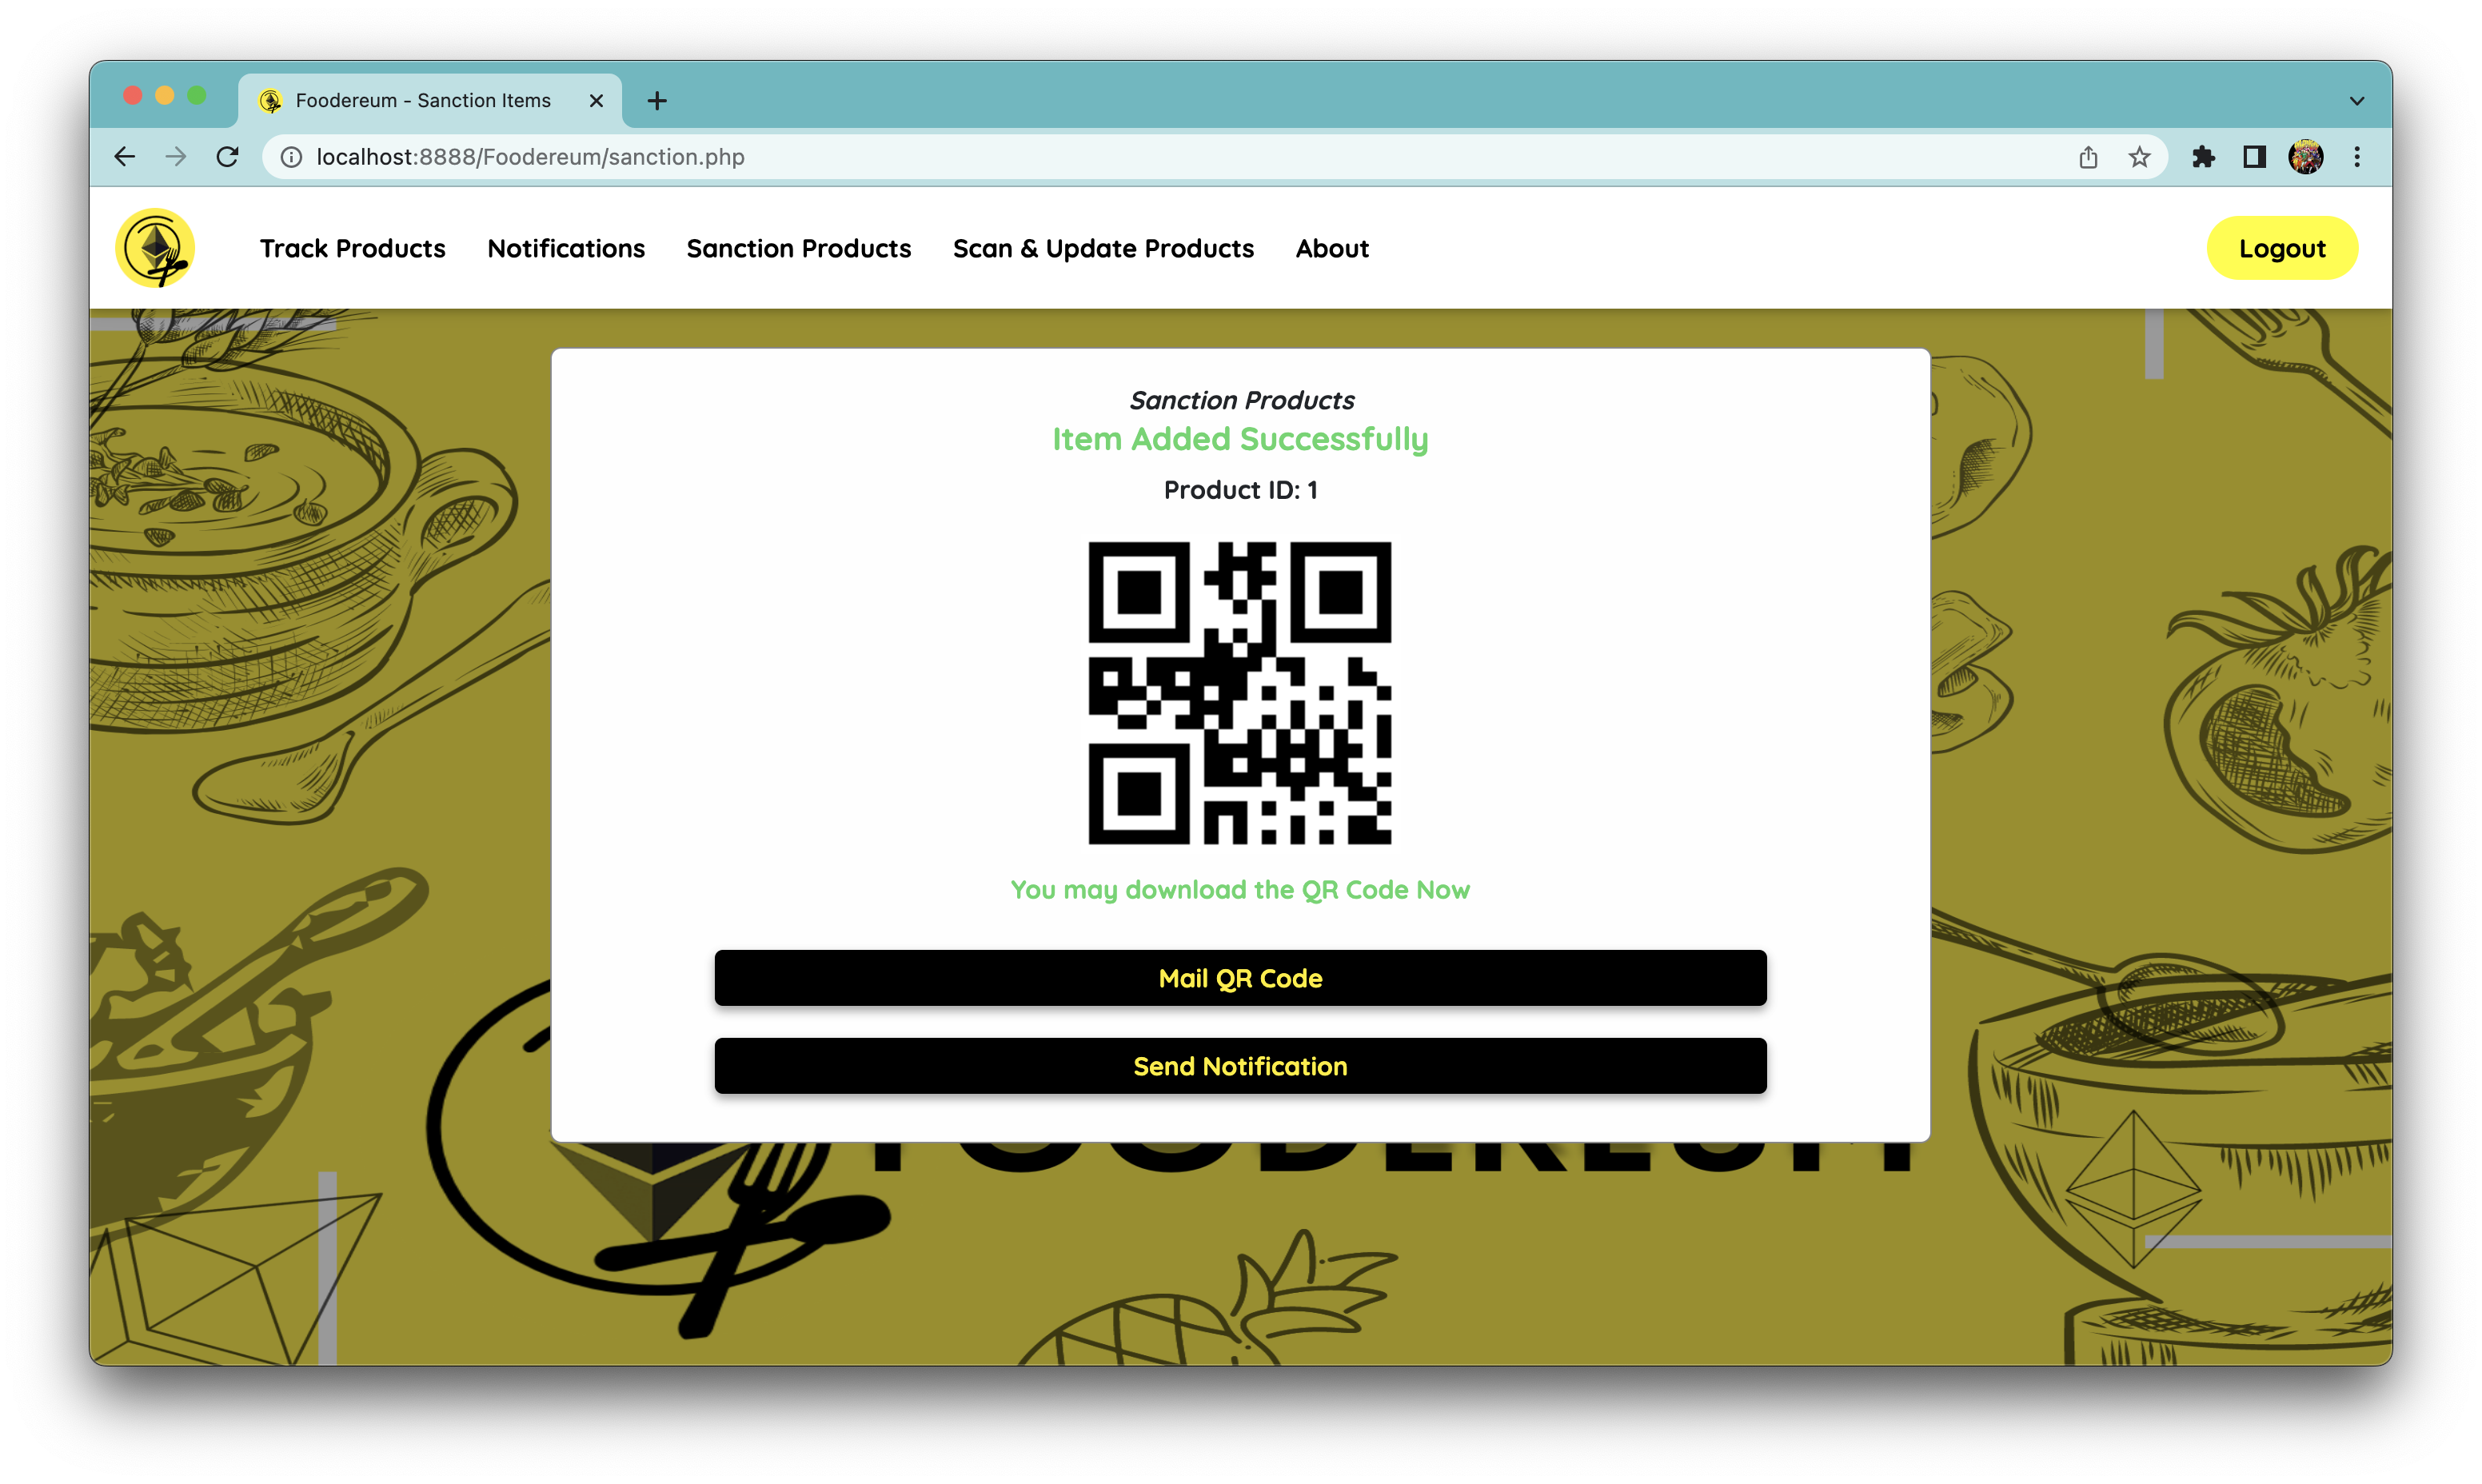
\includegraphics[width=15cm]{media/Rice_Sanctioned.png}
\centering
\caption{Sanctioning Rice}
\end{figure}
\begin{figure} [H]
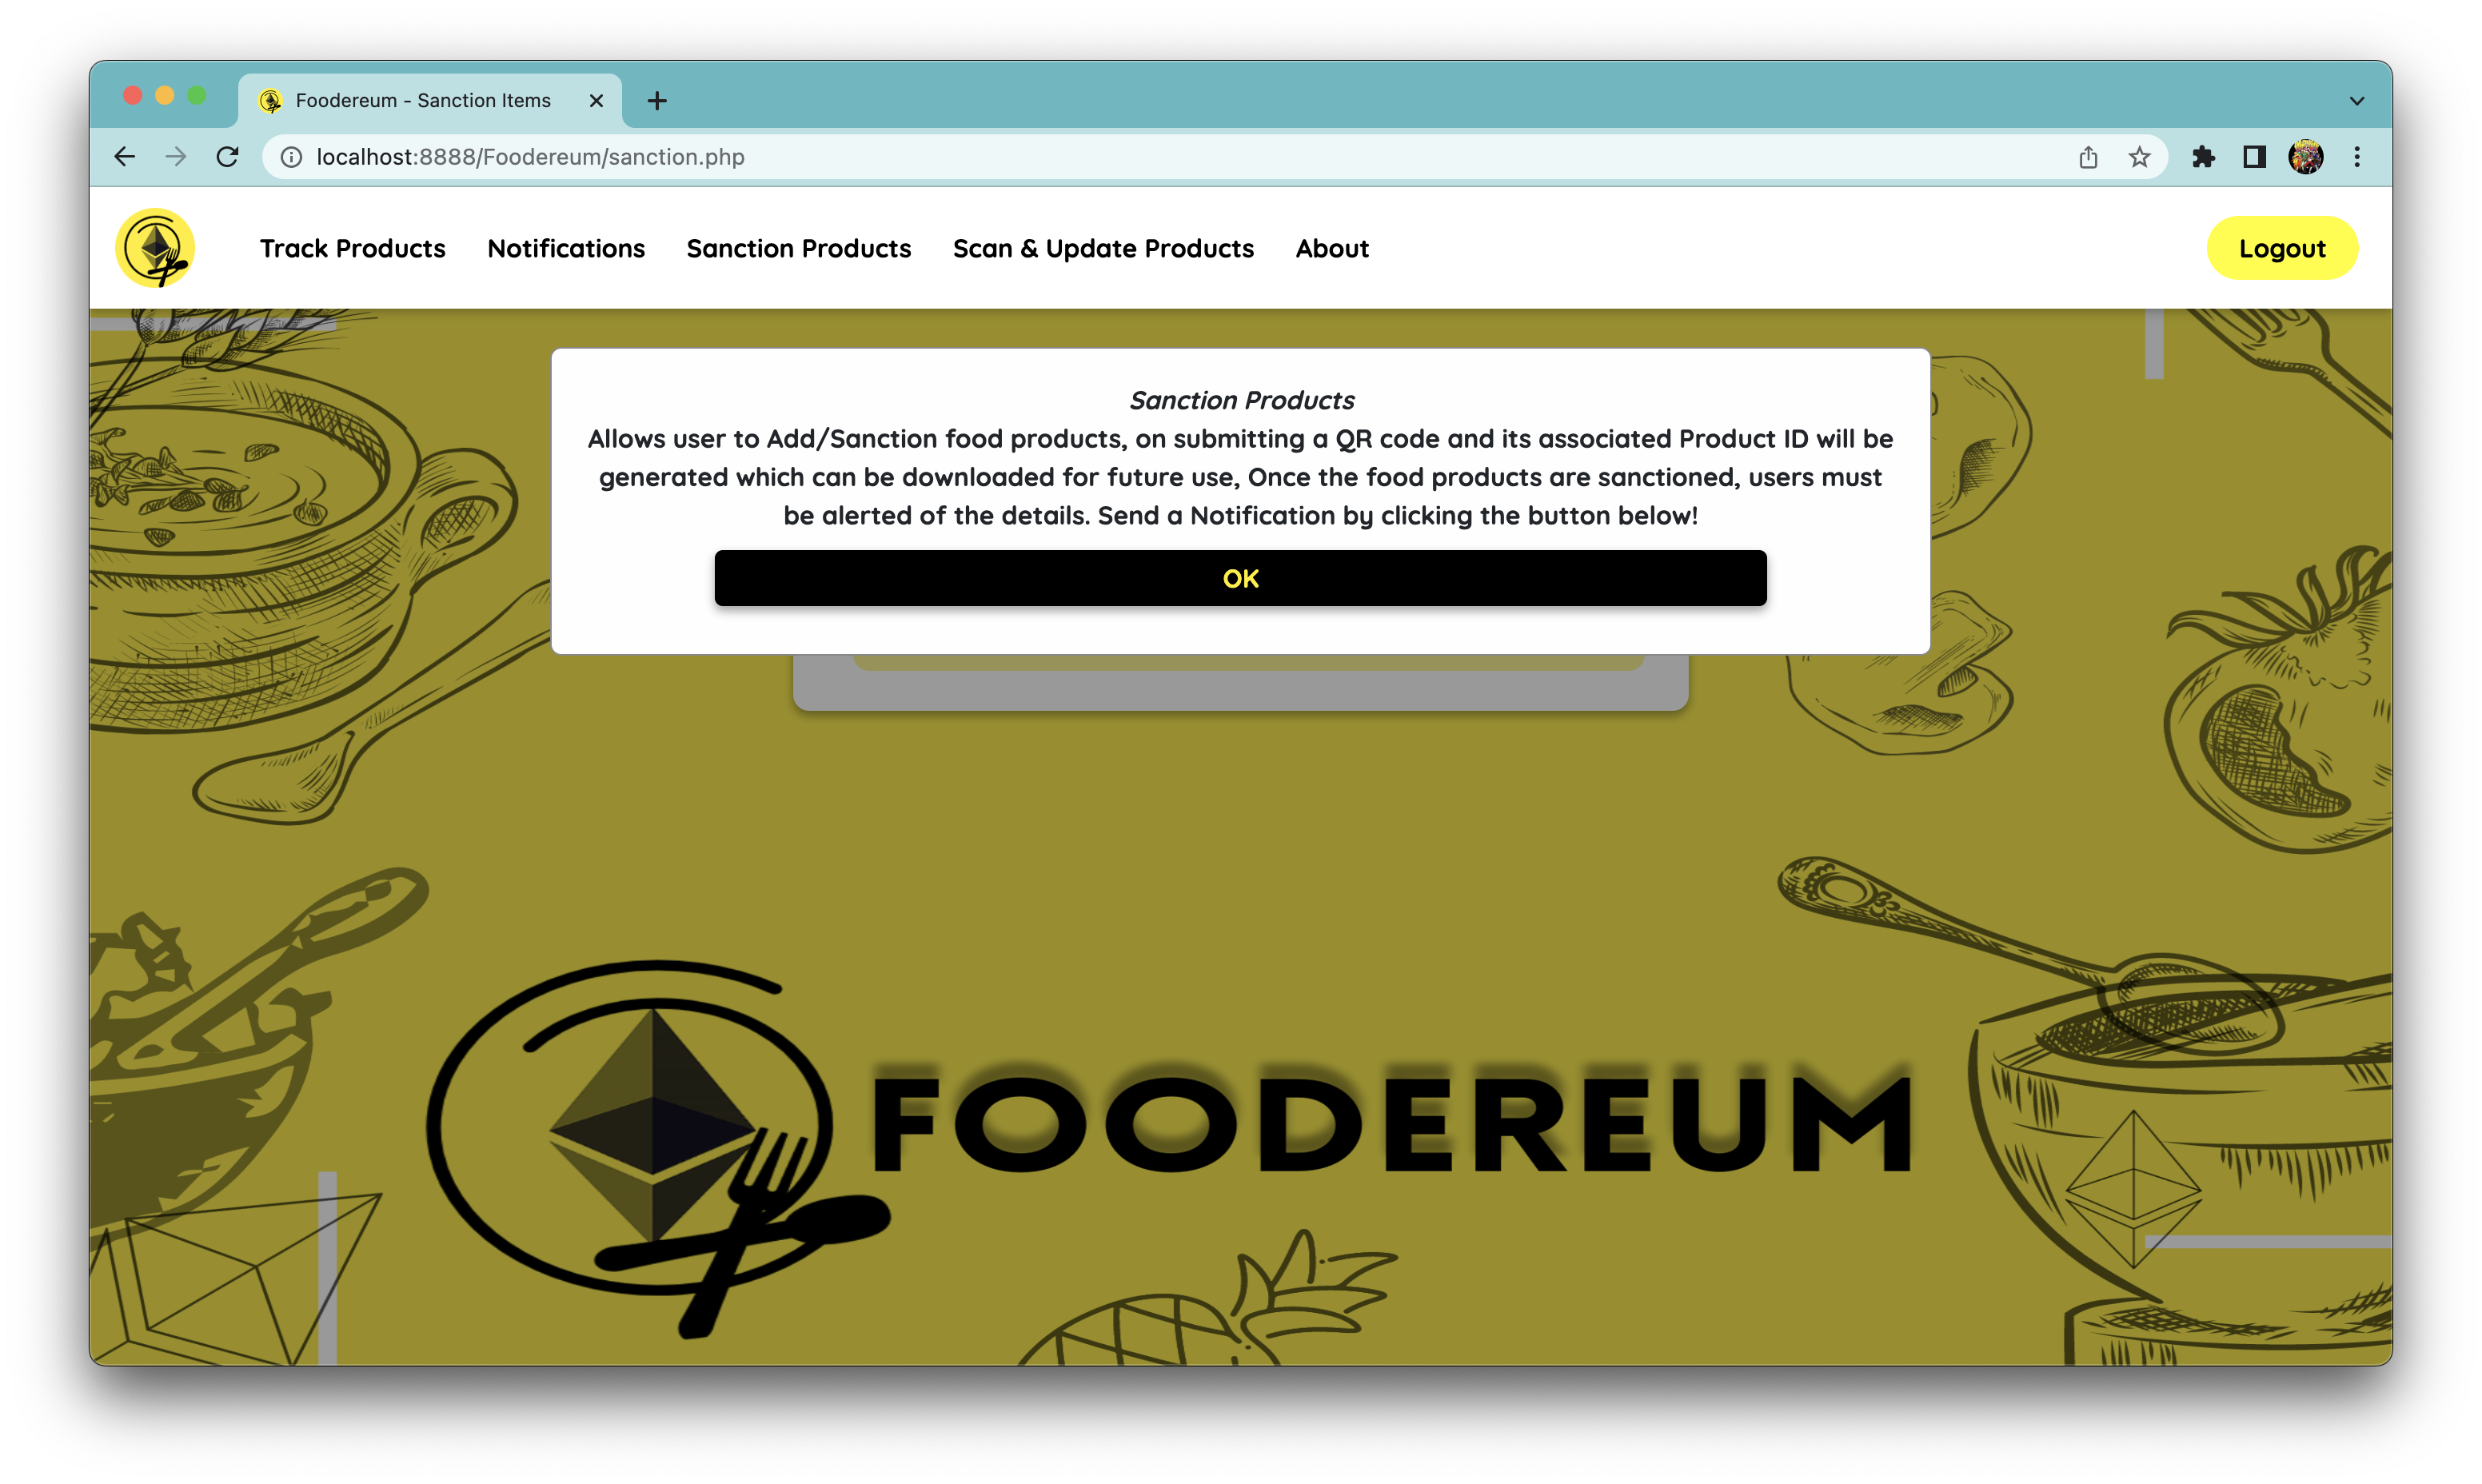
\includegraphics[width=15cm]{media/Sanction_About.png}
\centering
\caption{Sanction Products About Page}
\end{figure}
\begin{figure} [H]
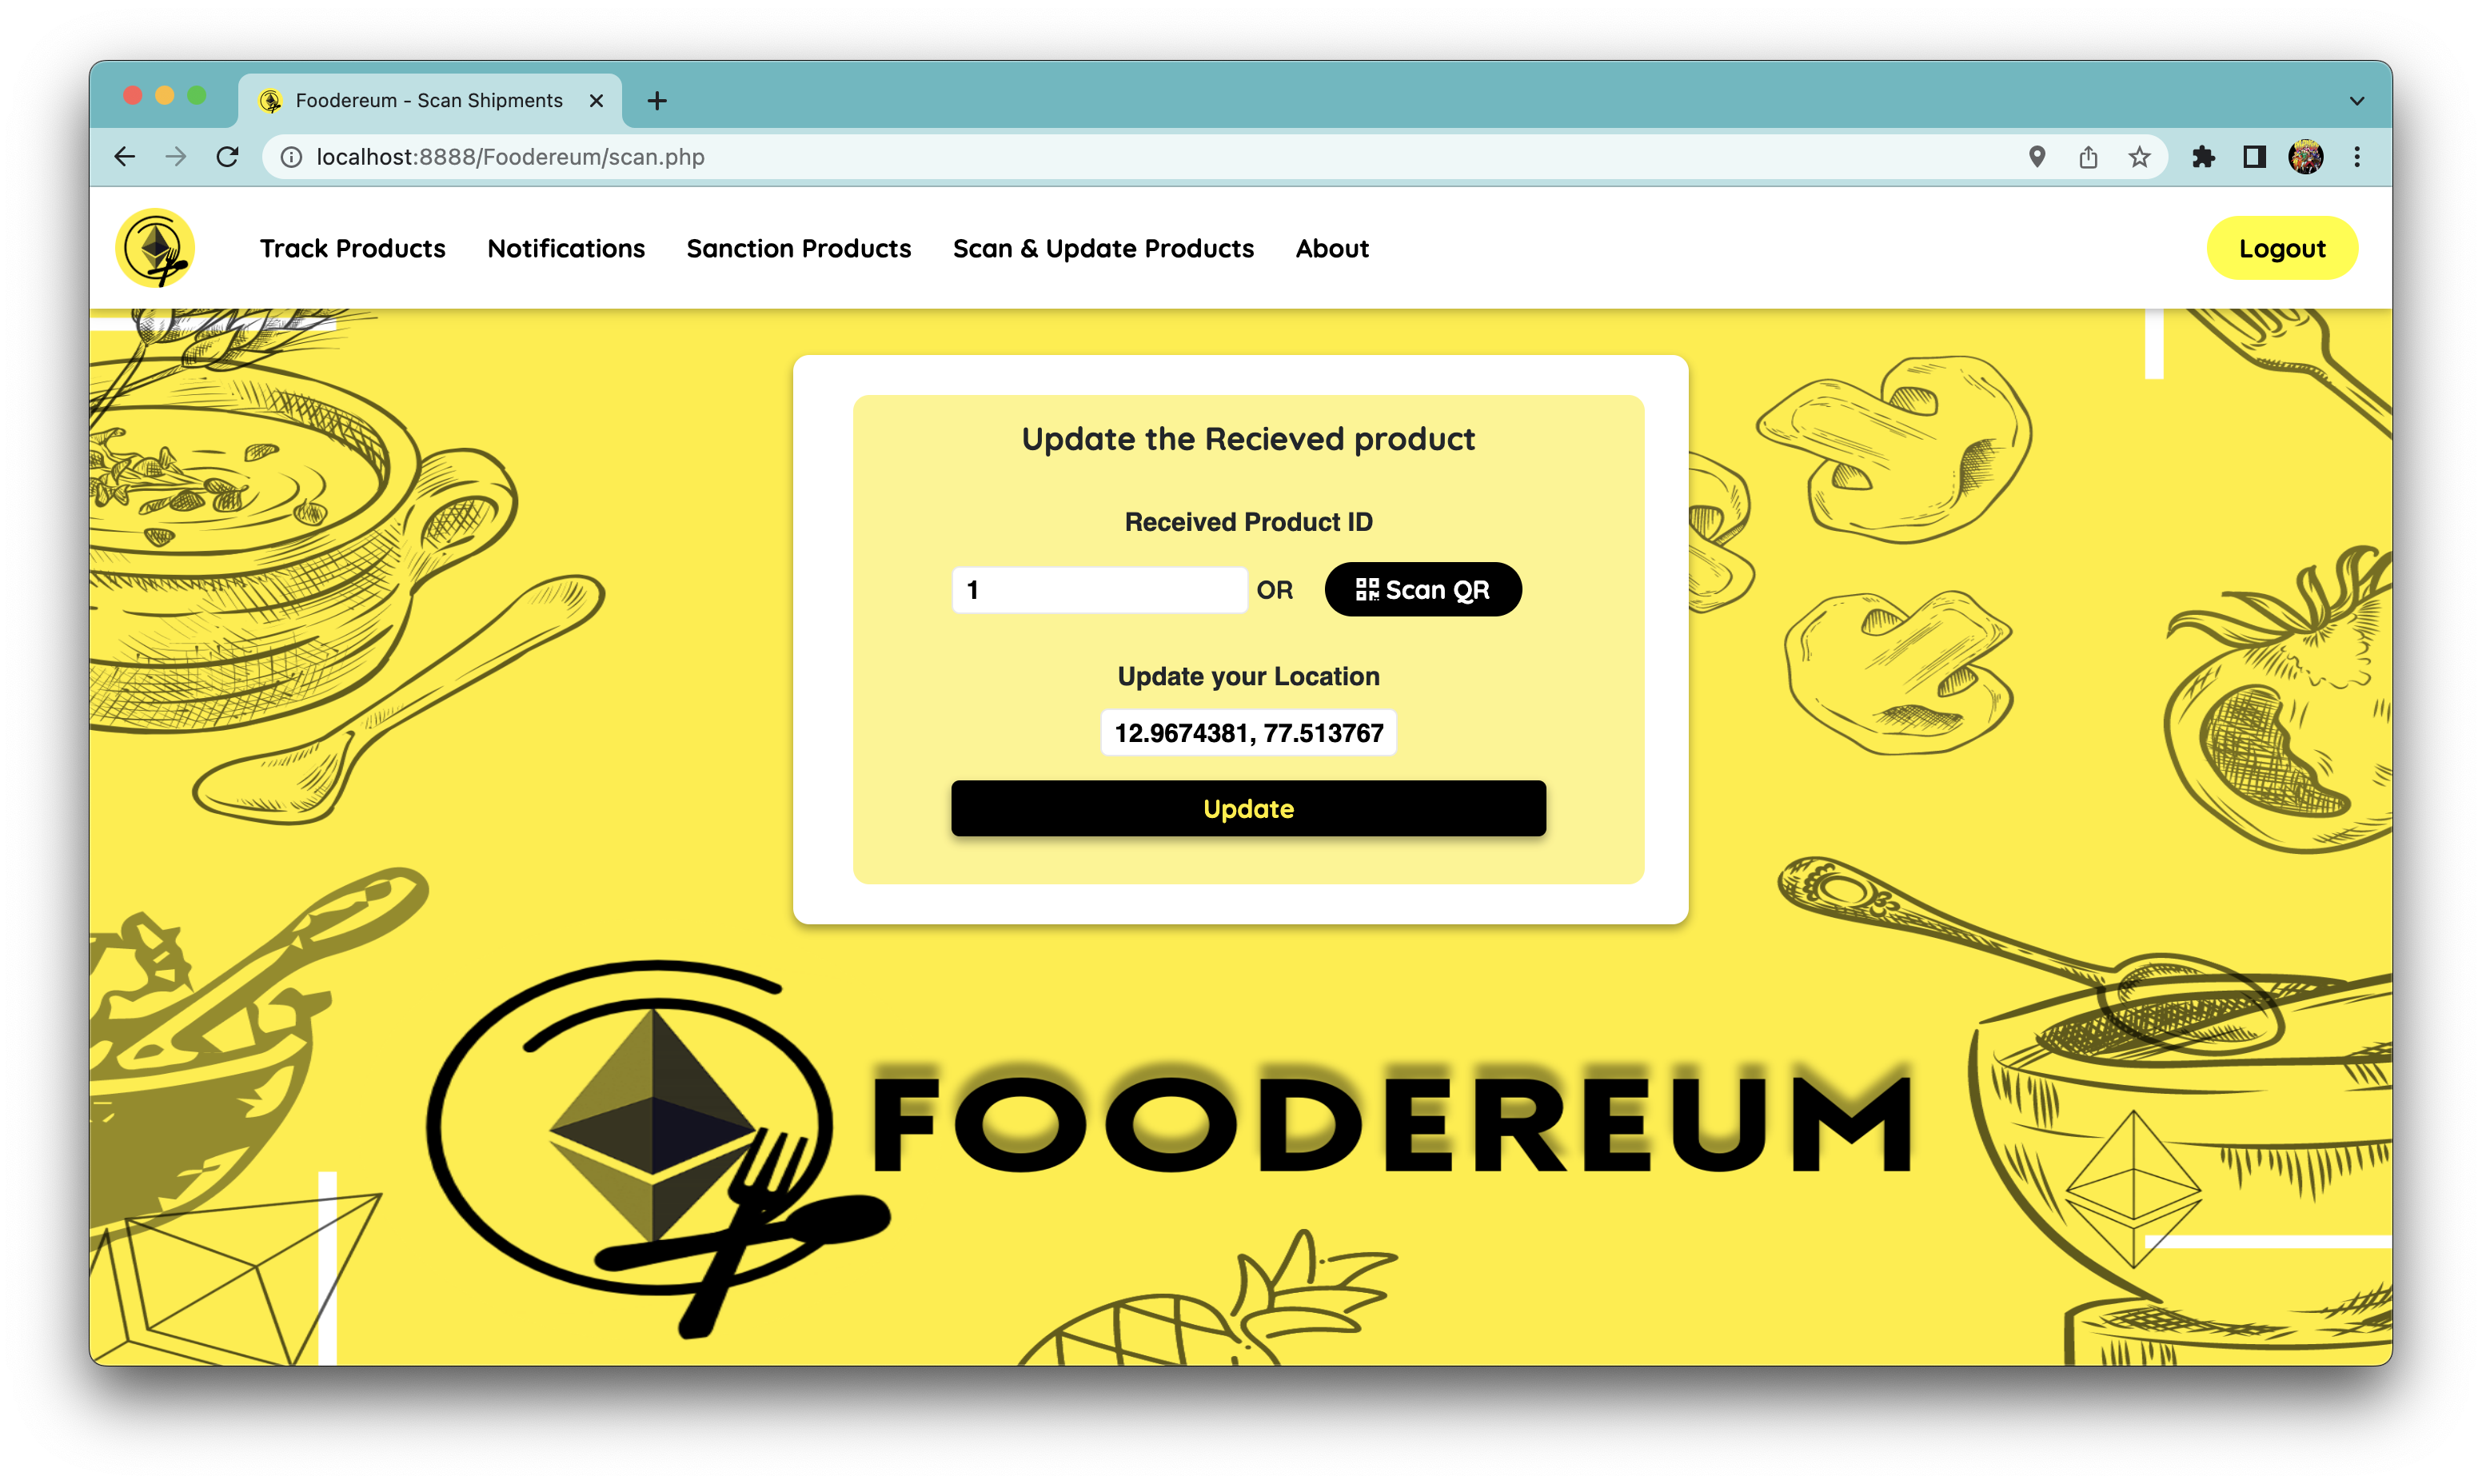
\includegraphics[width=15cm]{media/Scan.png}
\centering
\caption{Scan \& Update Products Page}
\end{figure}
\begin{figure} [H]
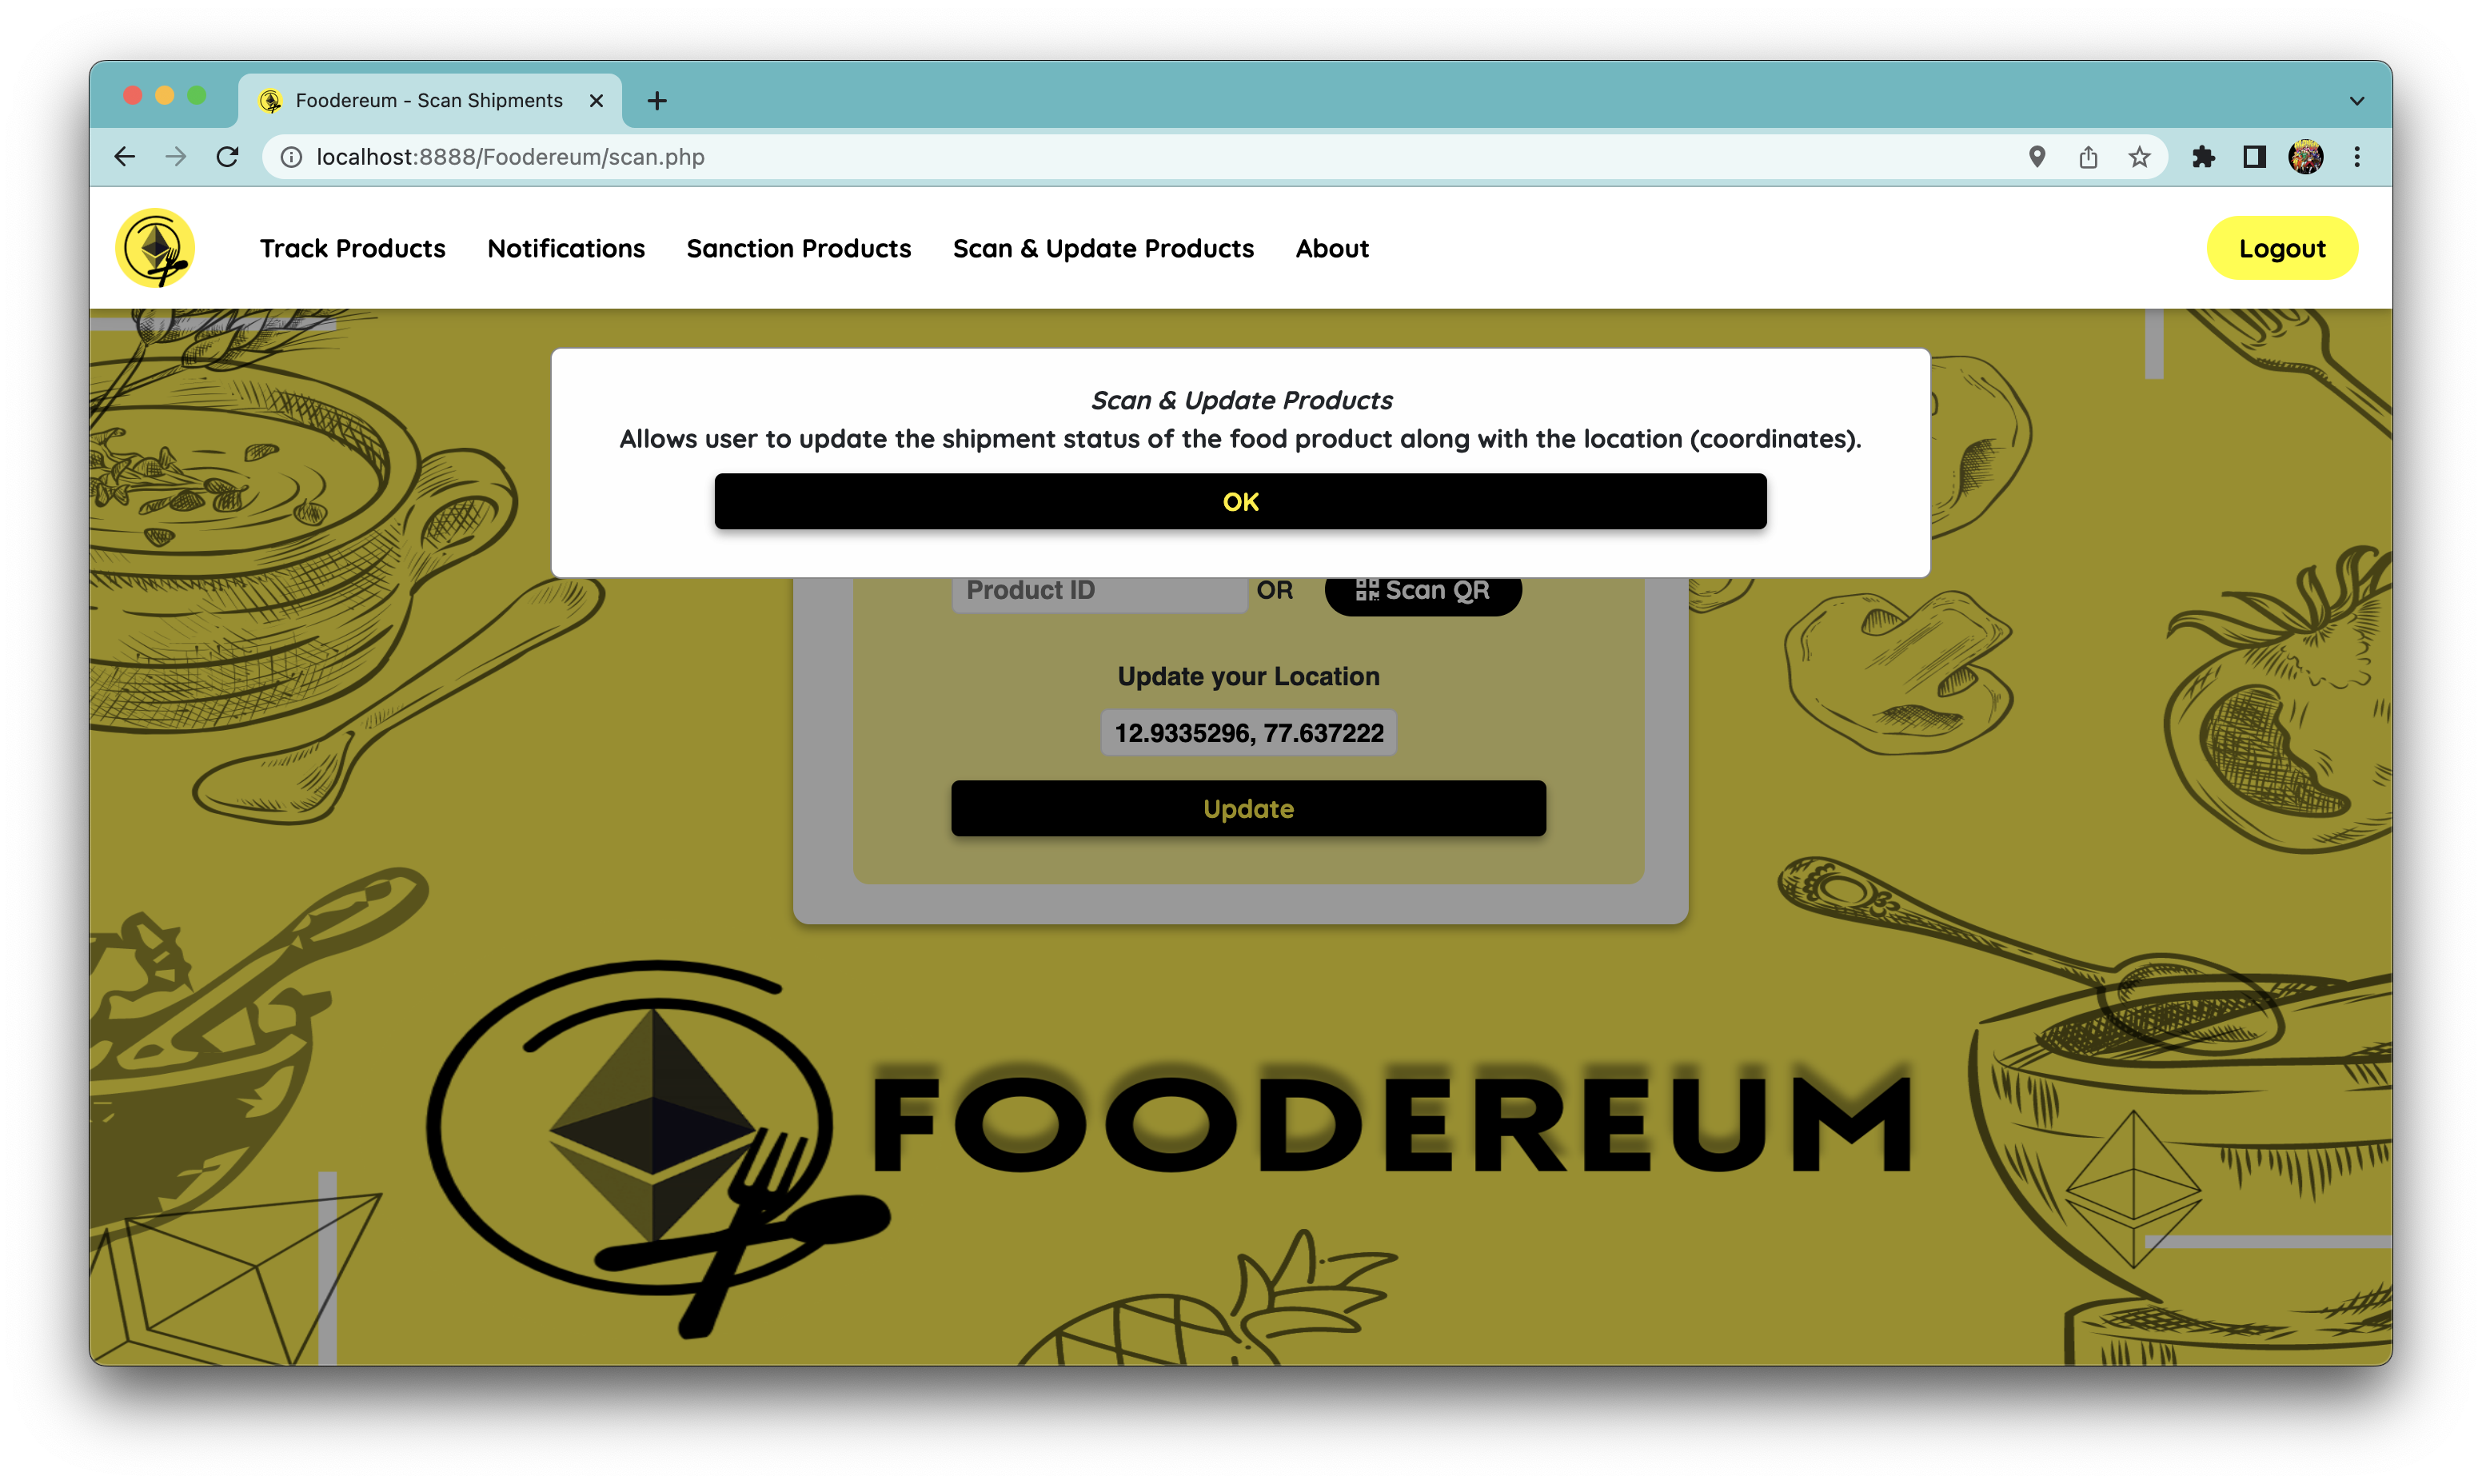
\includegraphics[width=15cm]{media/Scan_About.png}
\centering
\caption{Scan \& Update Products About Page}
\end{figure}
\begin{figure} [H]
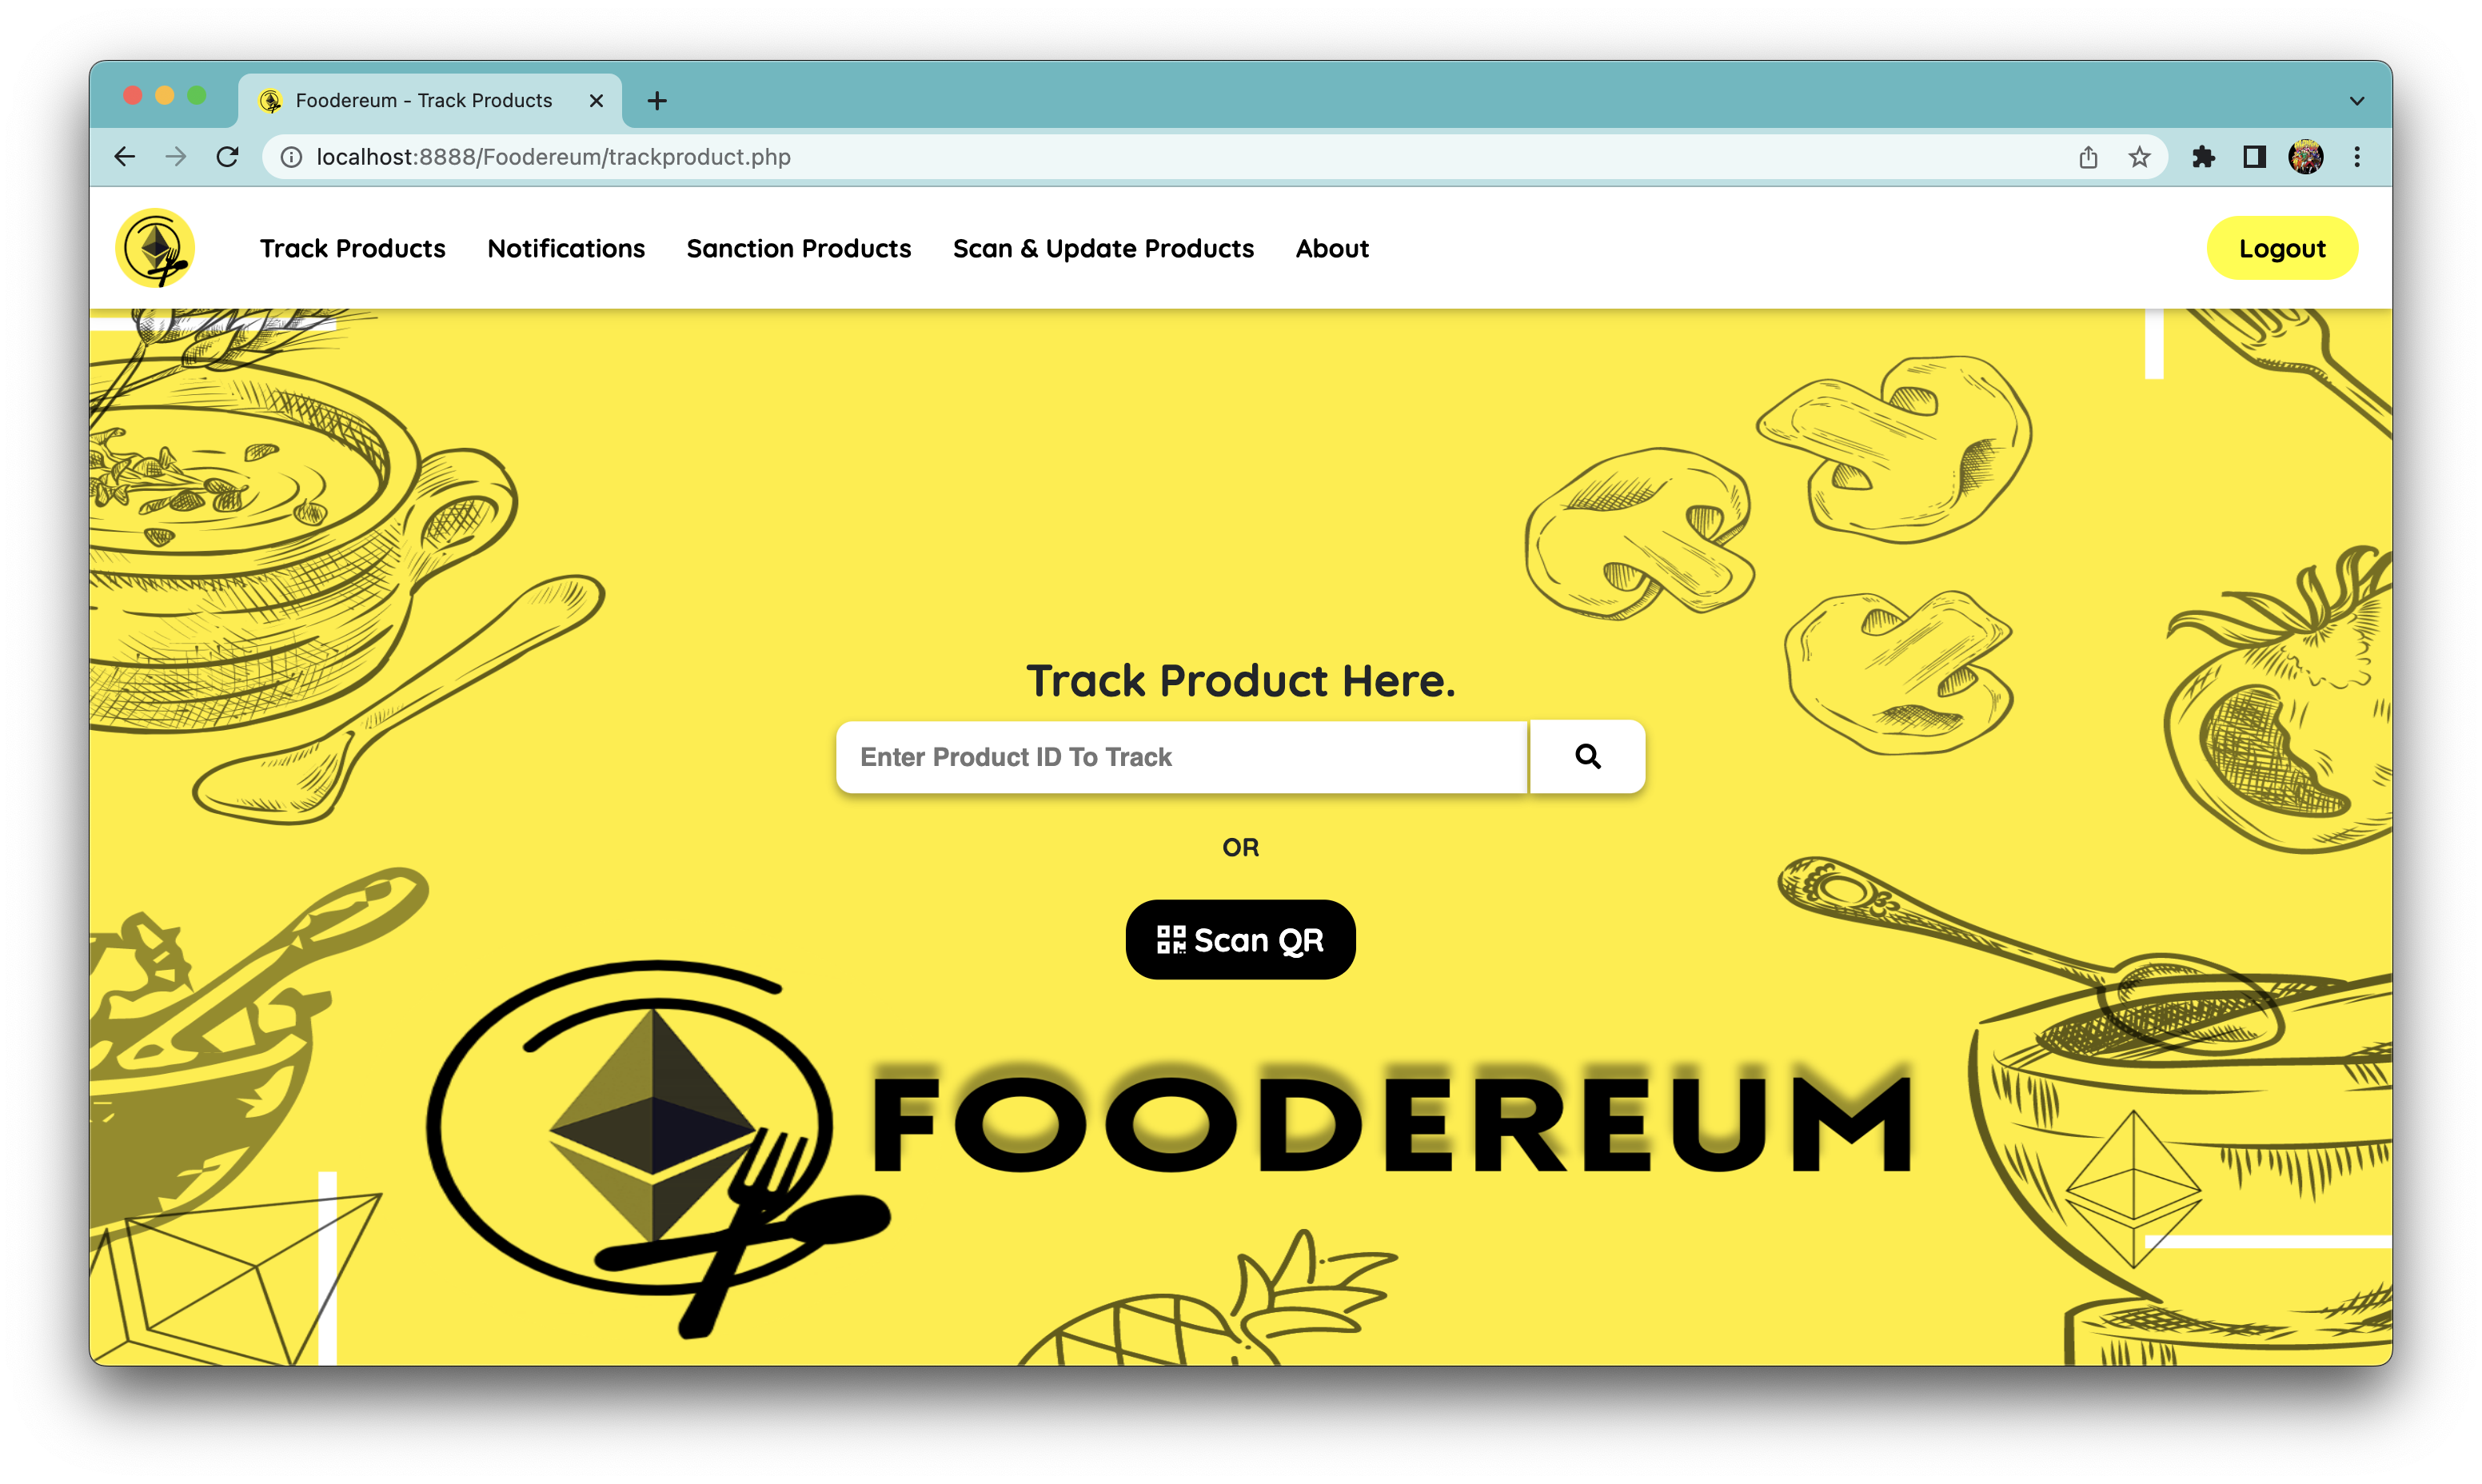
\includegraphics[width=15cm]{media/Track.png}
\centering
\caption{Track Products Page}
\end{figure}
\begin{figure} [H]
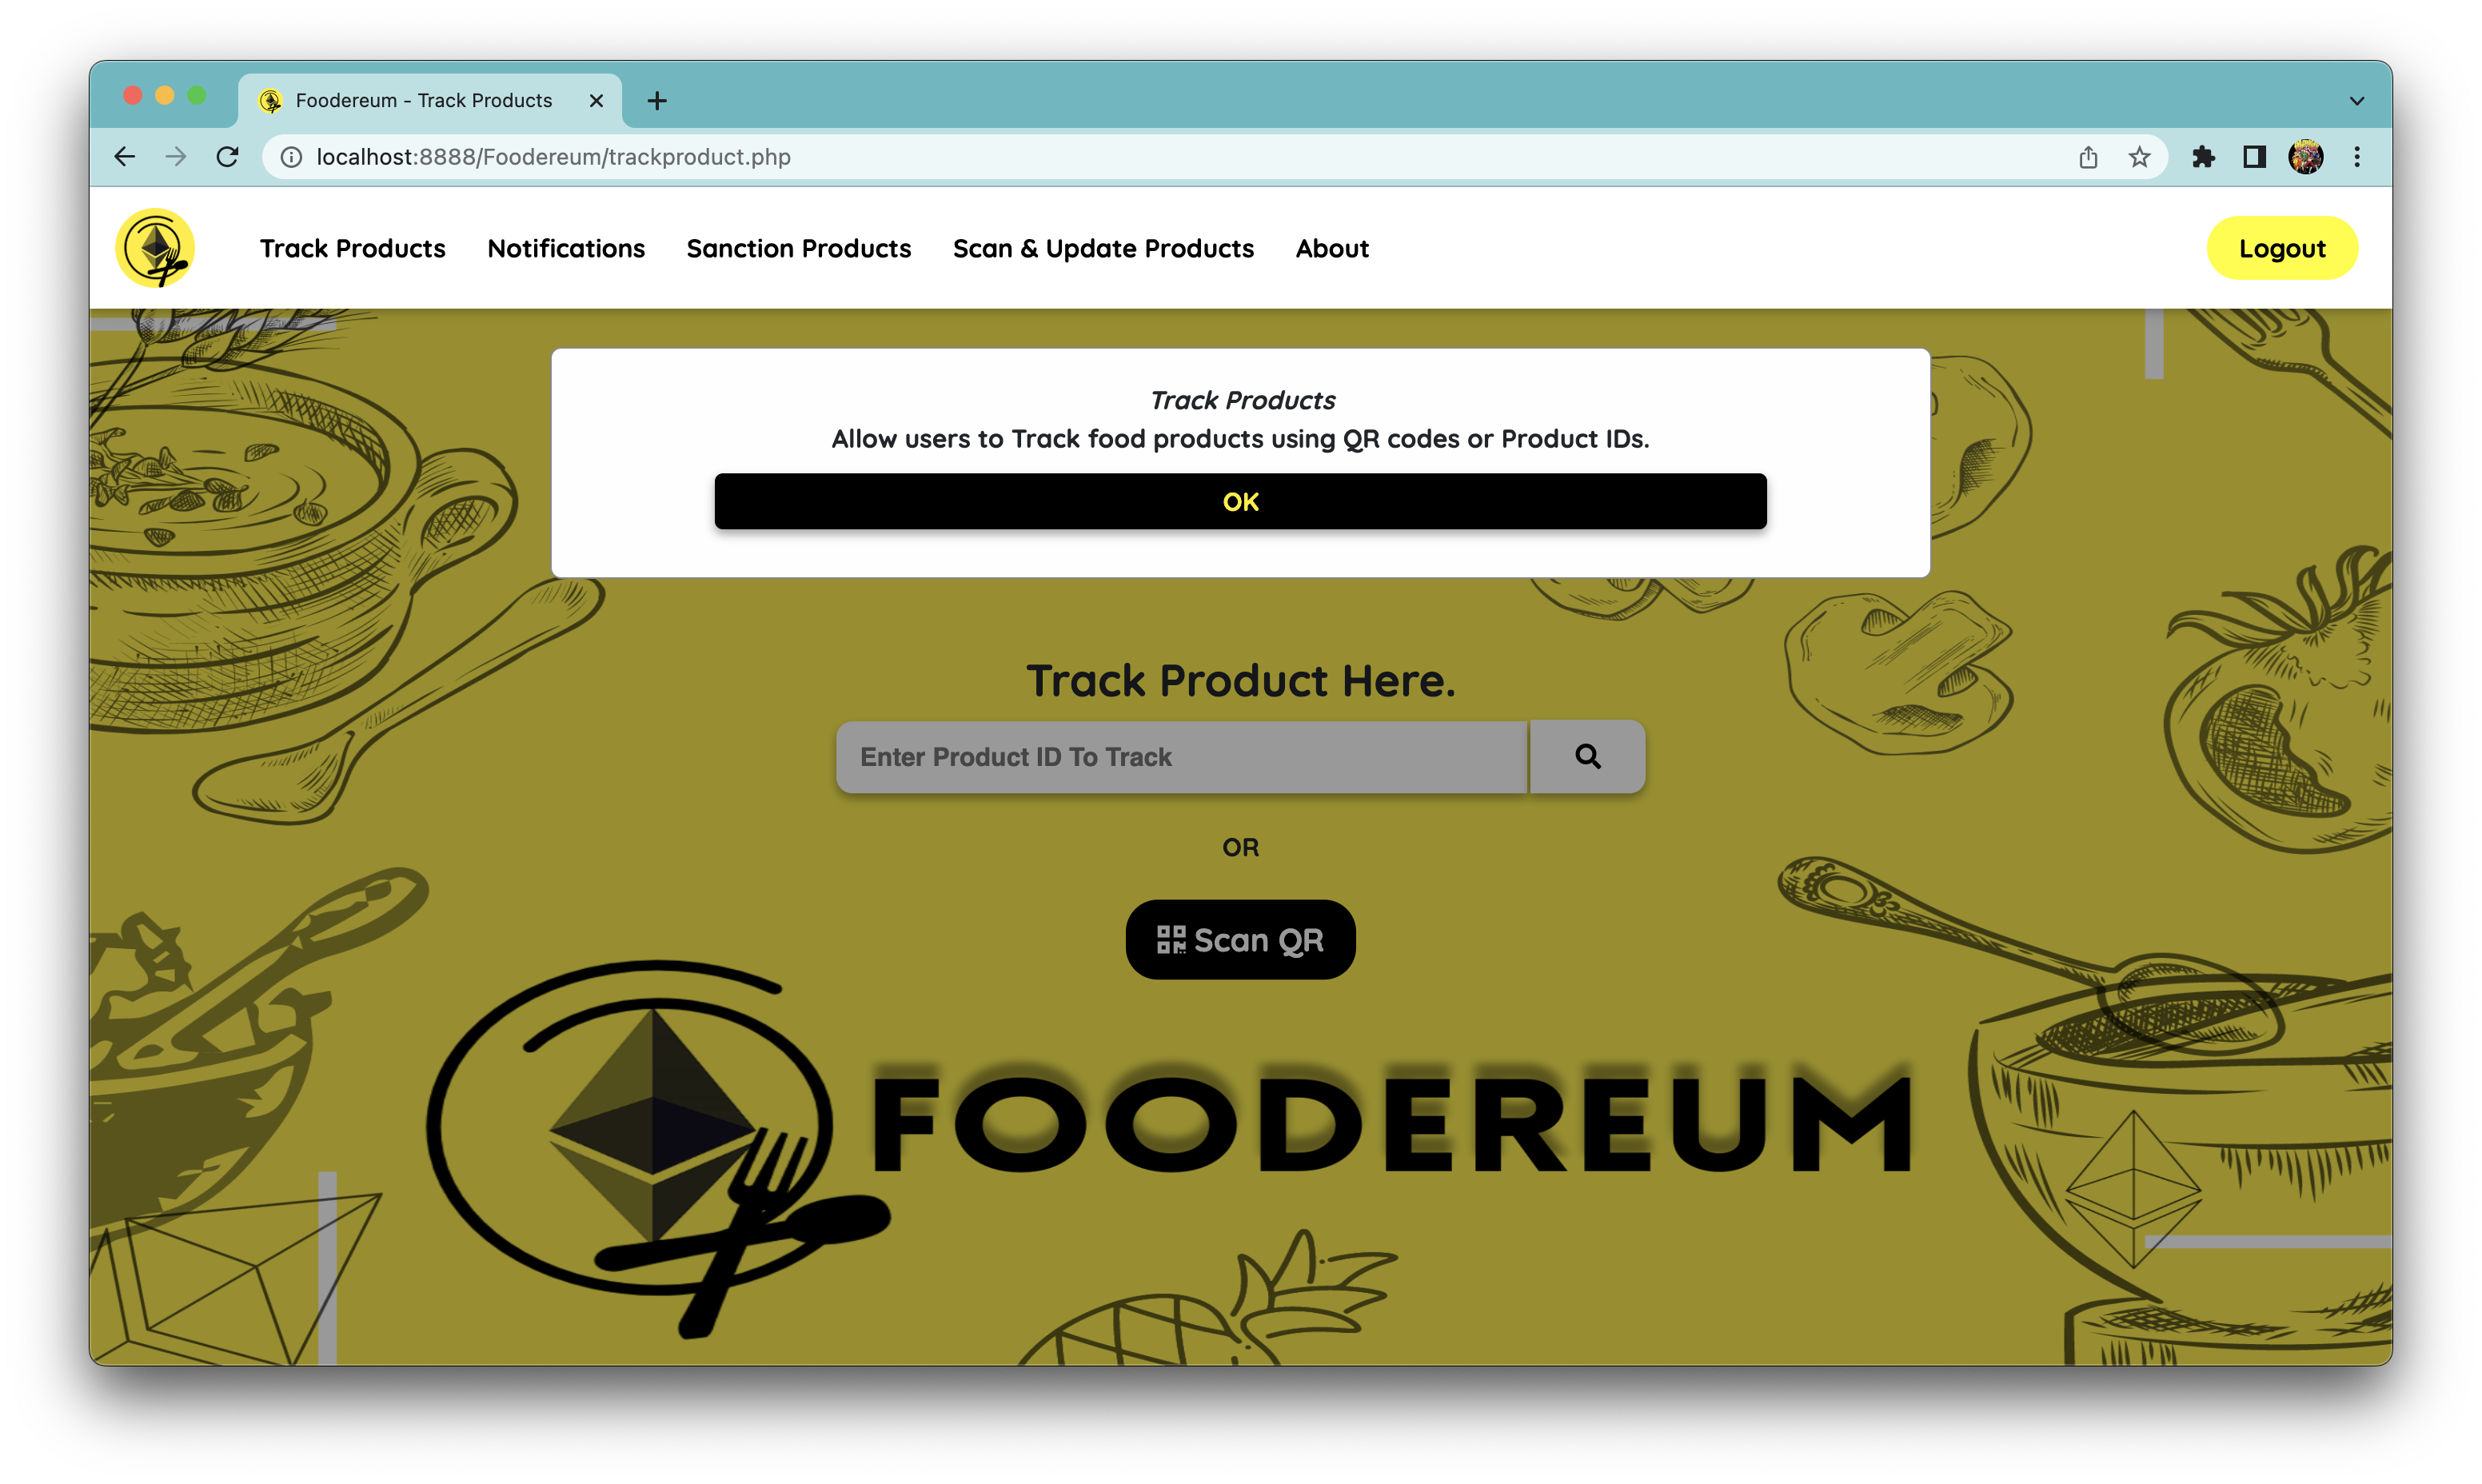
\includegraphics[width=15cm]{media/Track_About.png}
\centering
\caption{Track Products About Page}
\end{figure}
\begin{figure} [H]
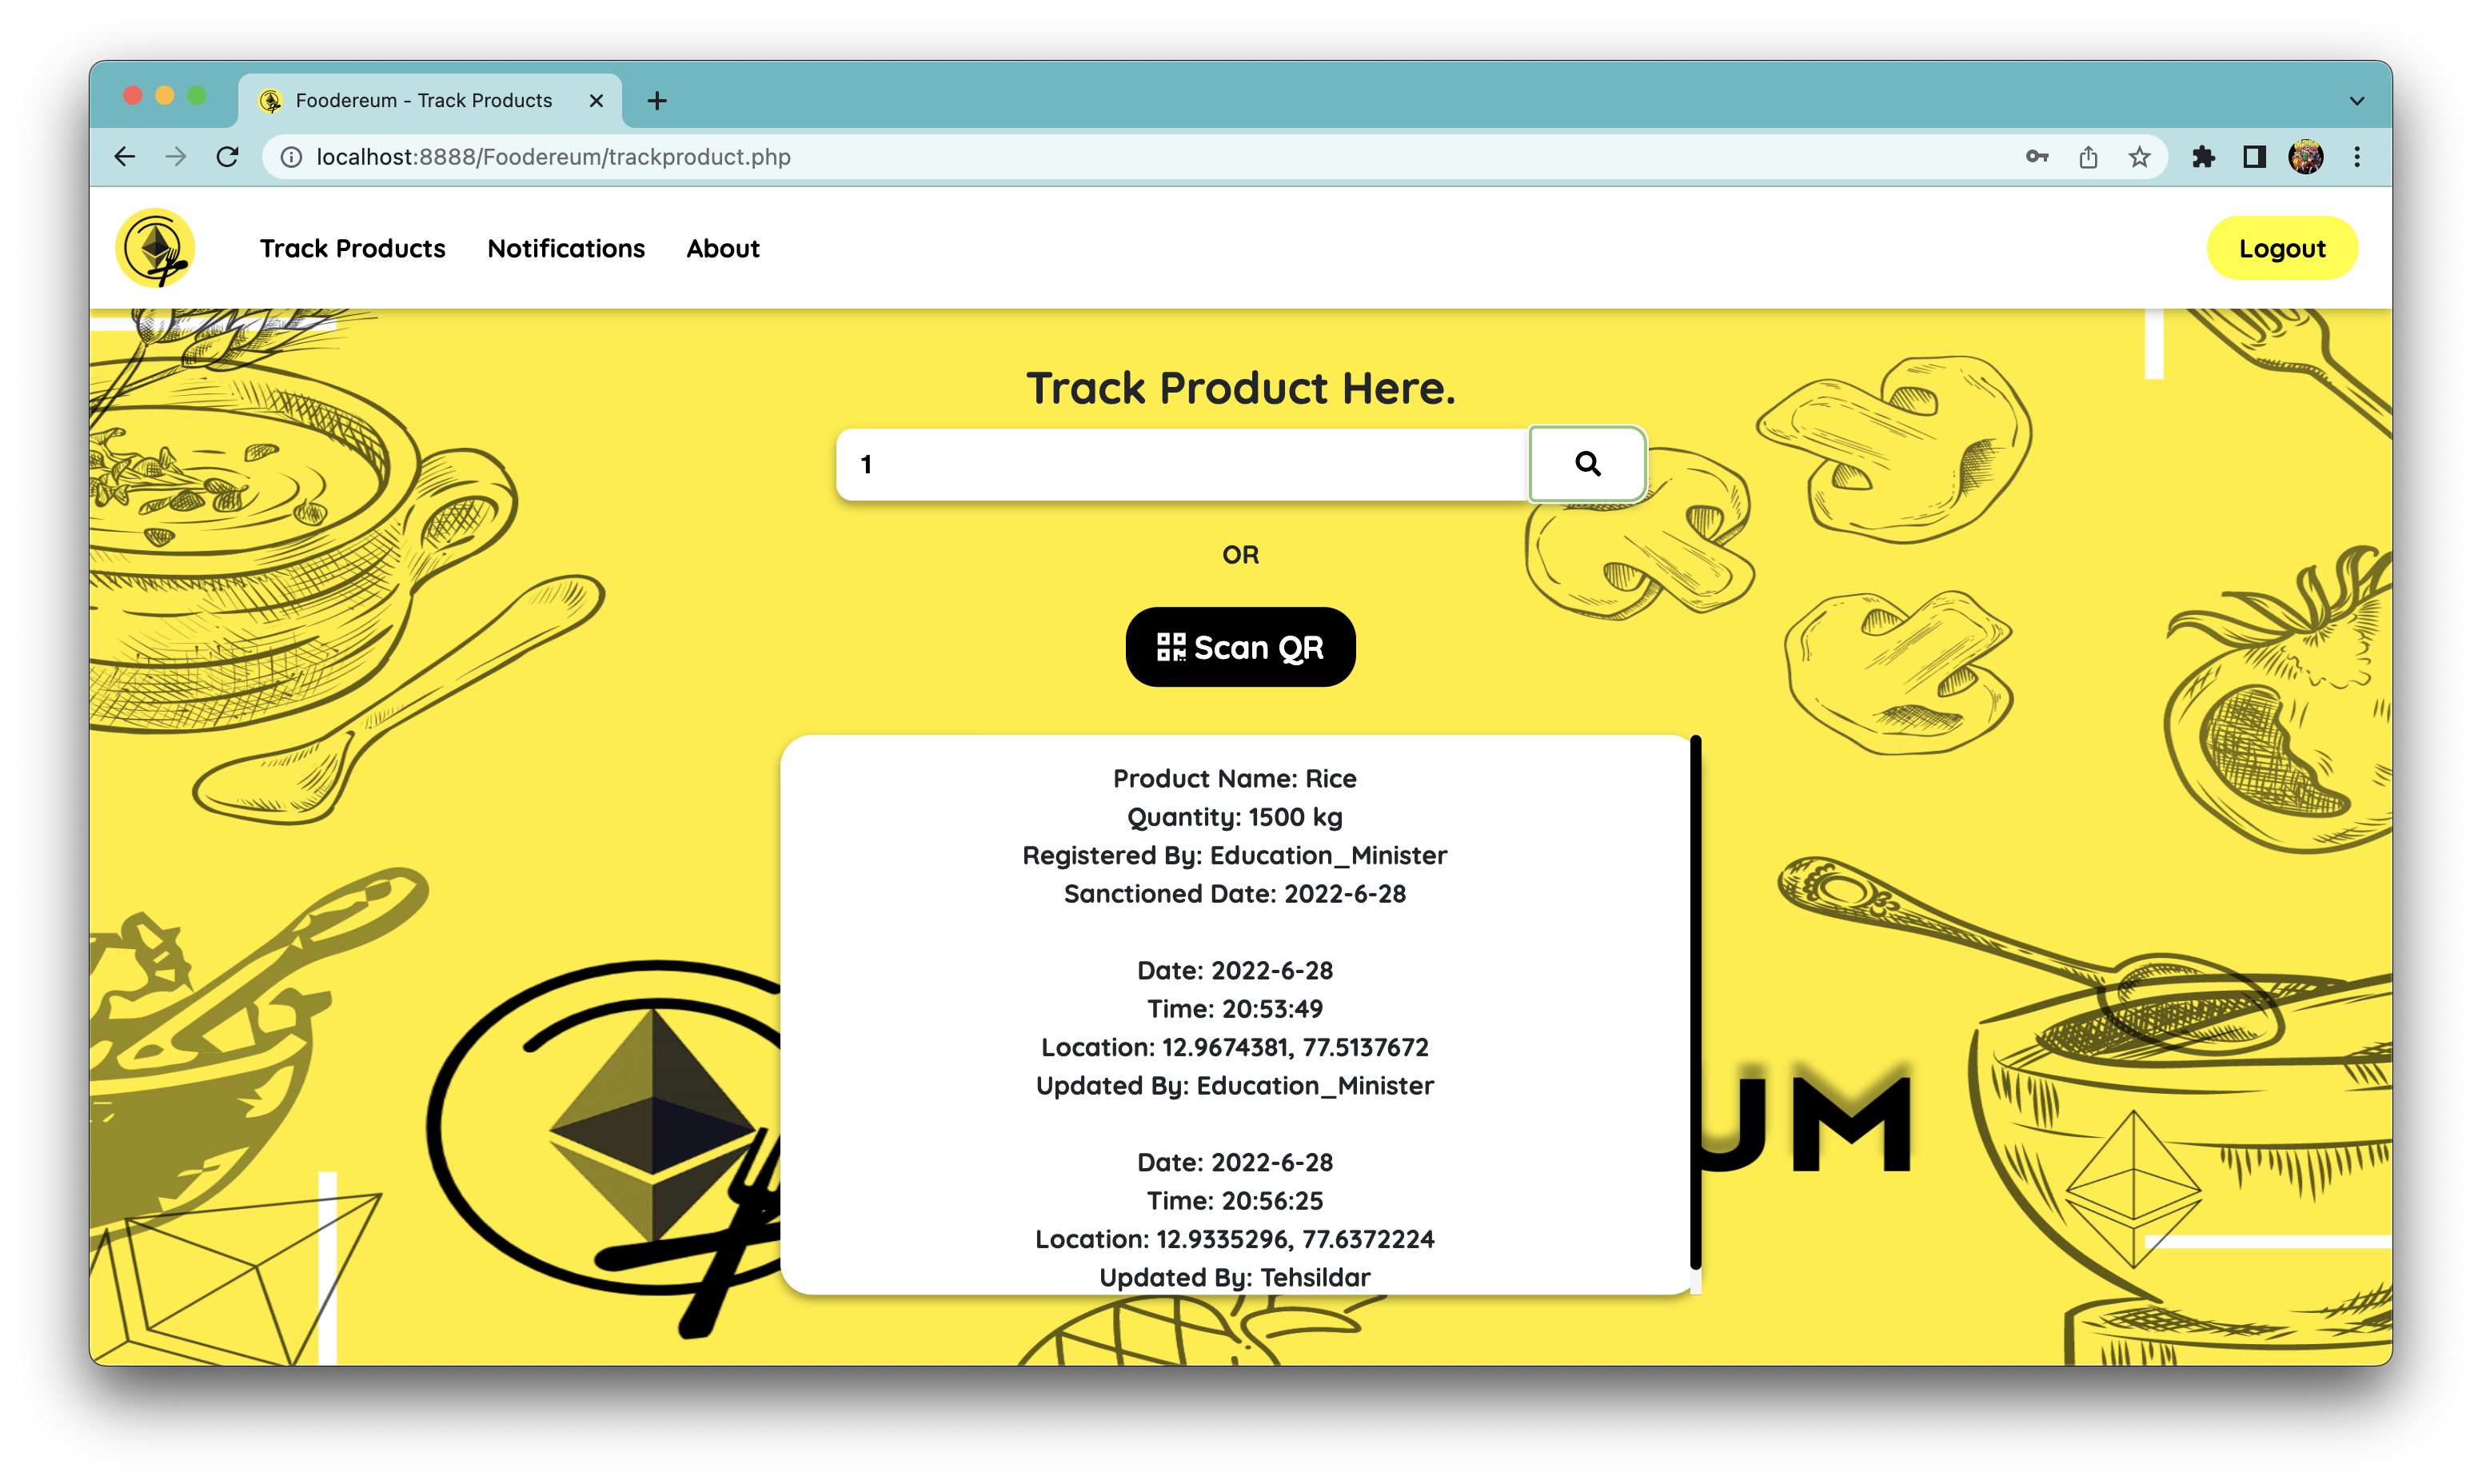
\includegraphics[width=15cm]{media/Rice_Track.png}
\centering
\caption{Tracking Rice}
\end{figure}
\begin{figure} [H]
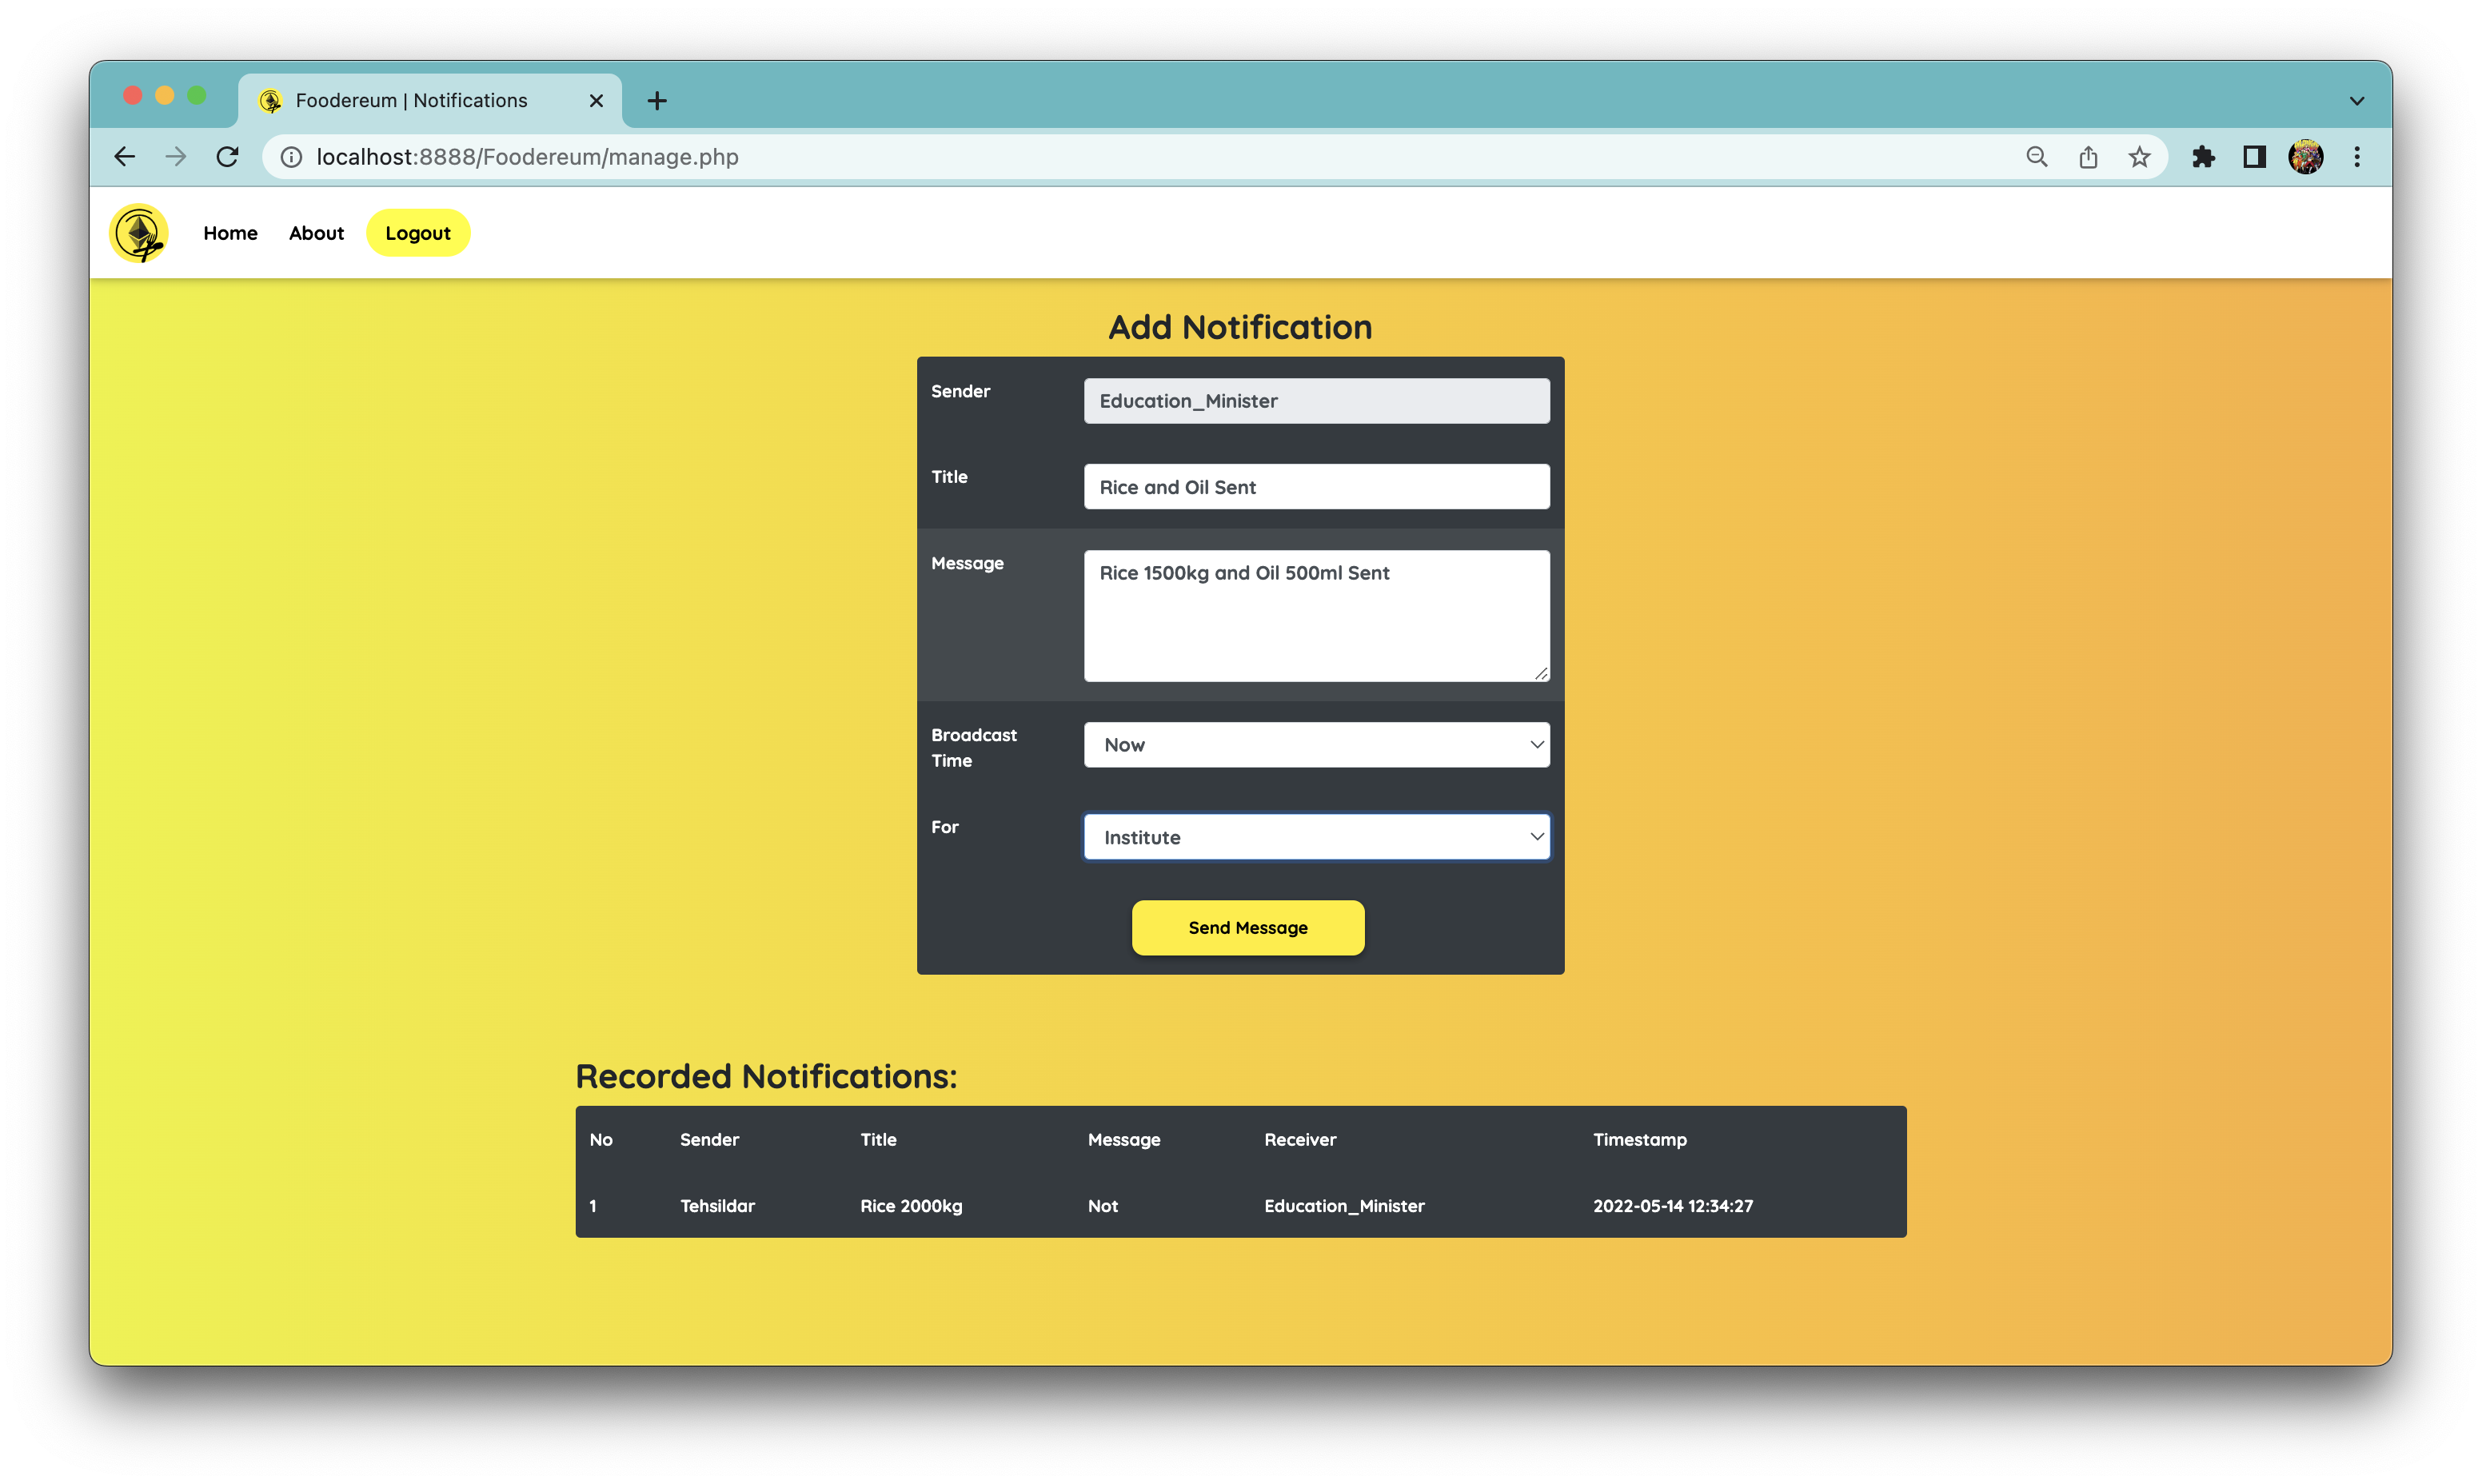
\includegraphics[width=15cm]{media/Notification.png}
\centering
\caption{Notifications Page}
\end{figure}
\begin{figure} [H]
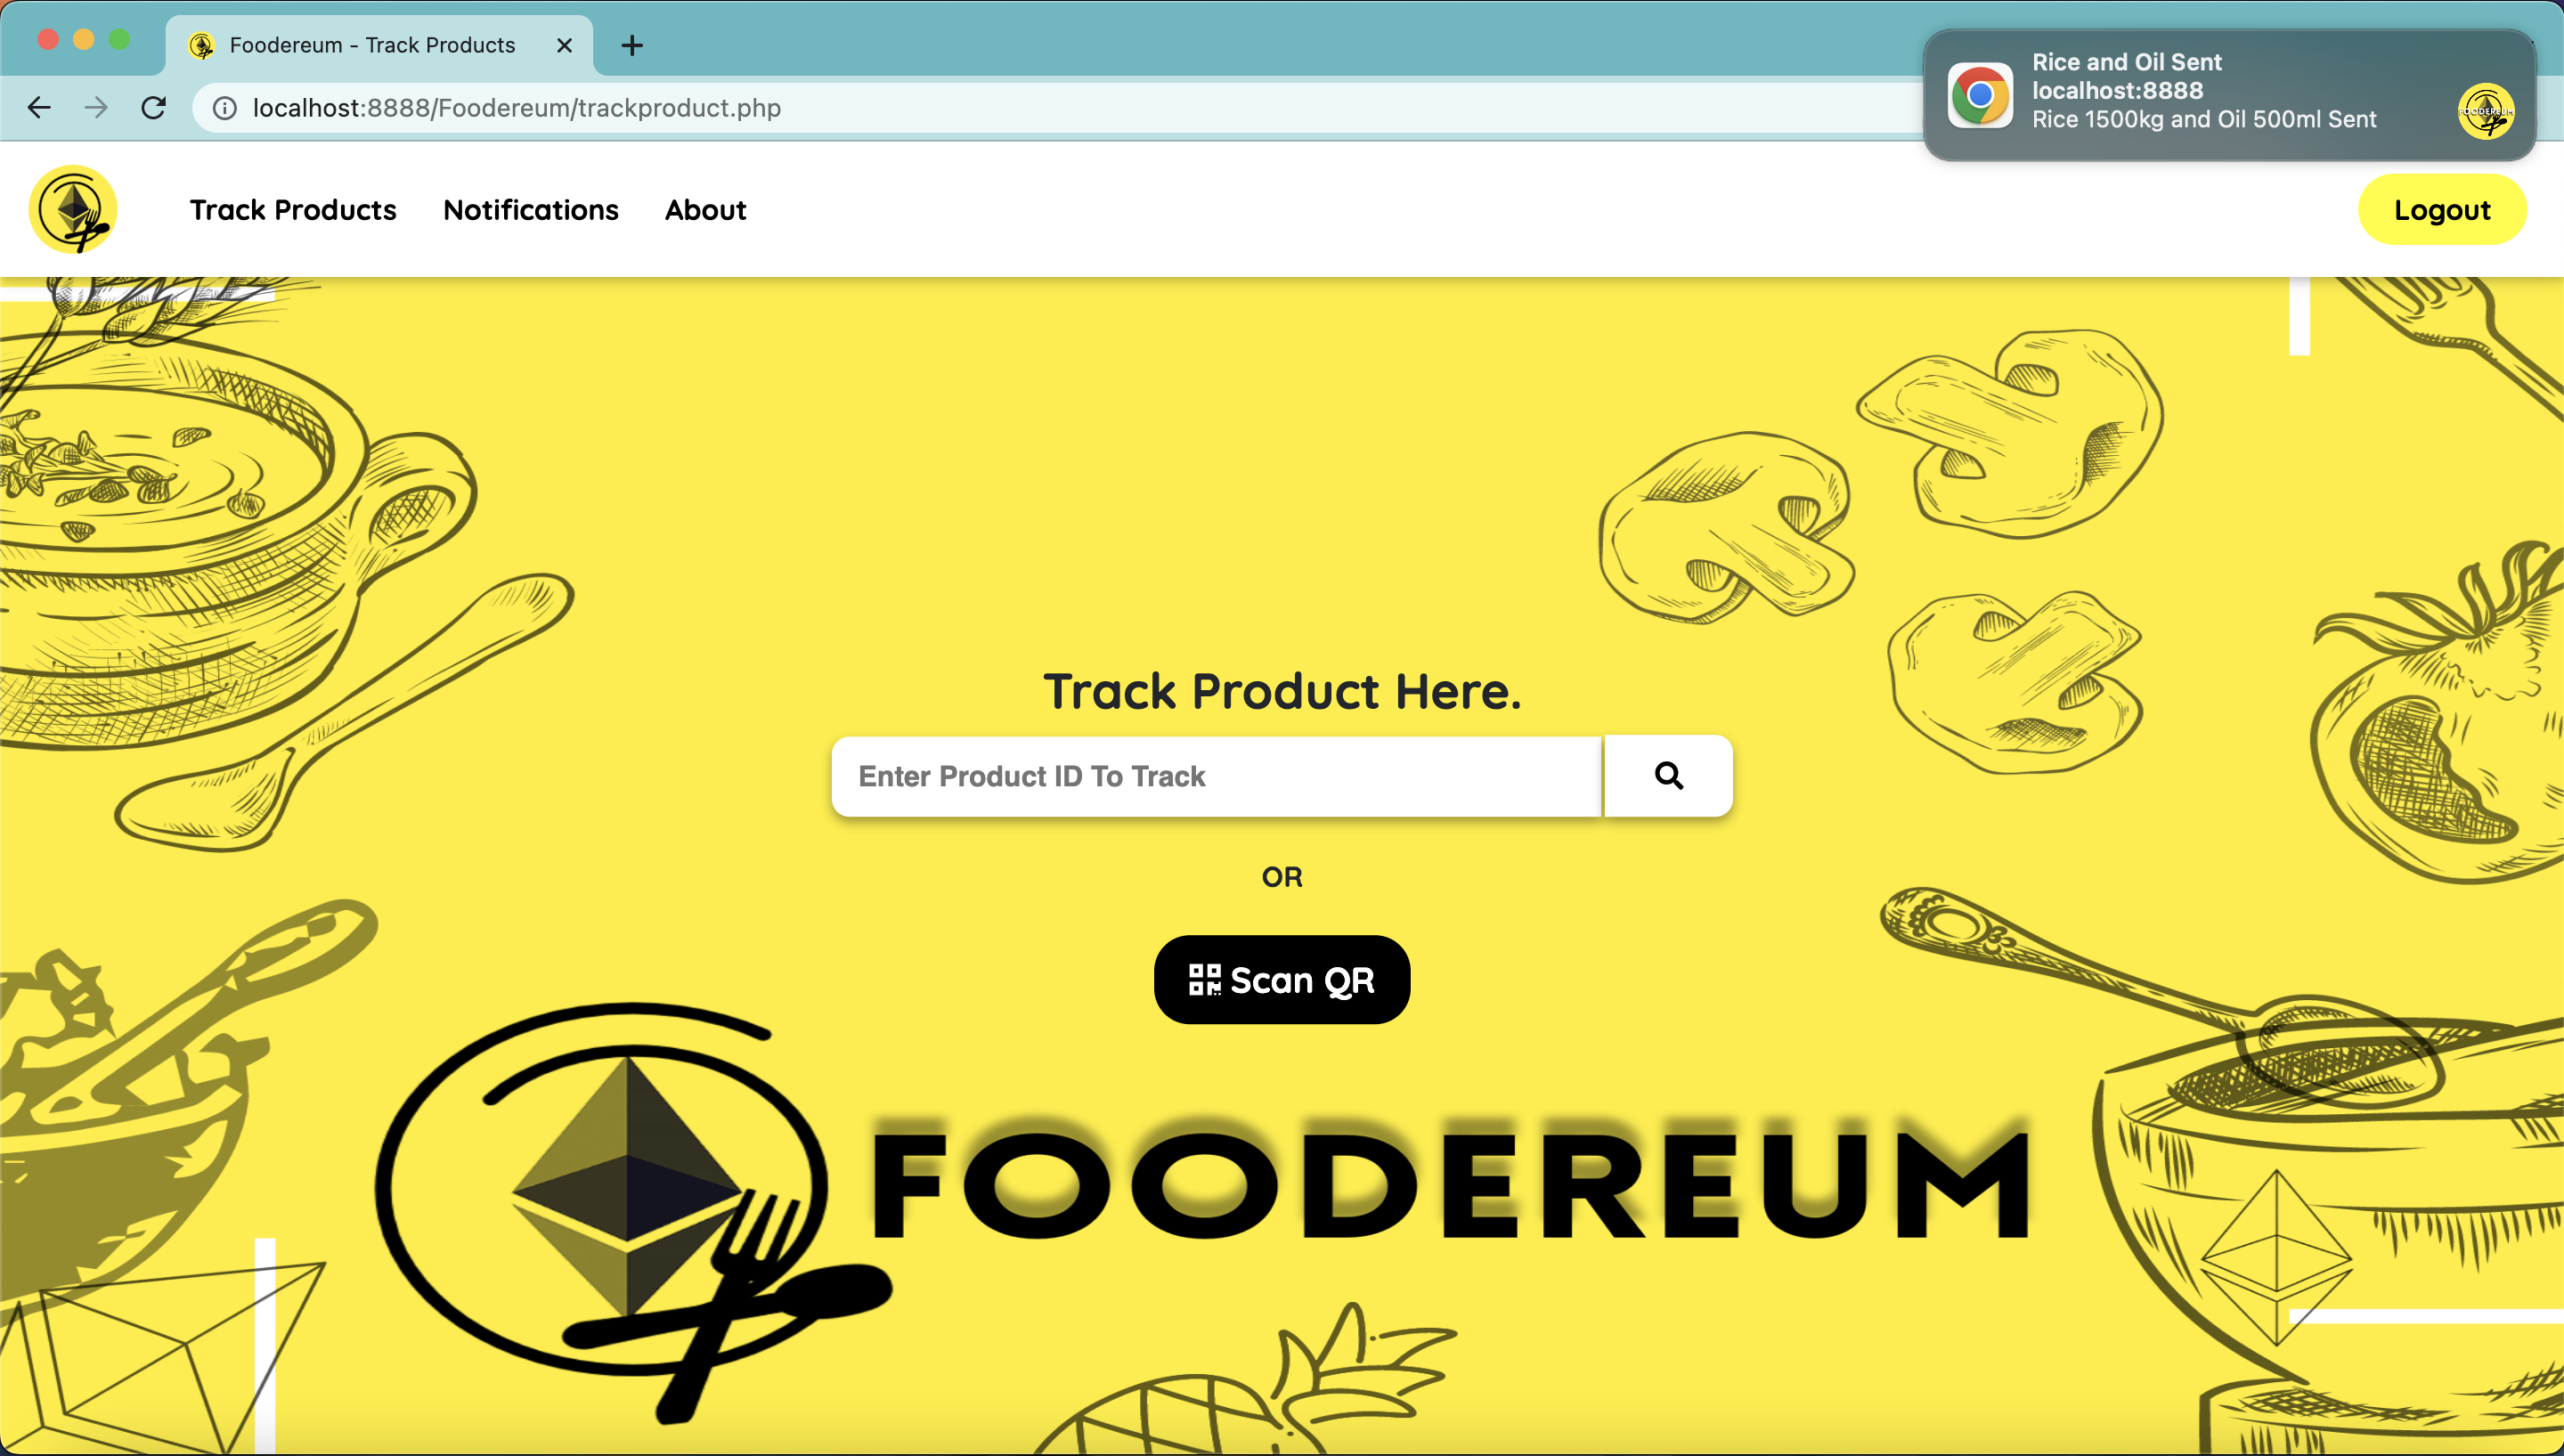
\includegraphics[width=15cm]{media/Notif_Received.png}
\centering
\caption{Push Notification Alert}
\end{figure}
\begin{figure} [H]
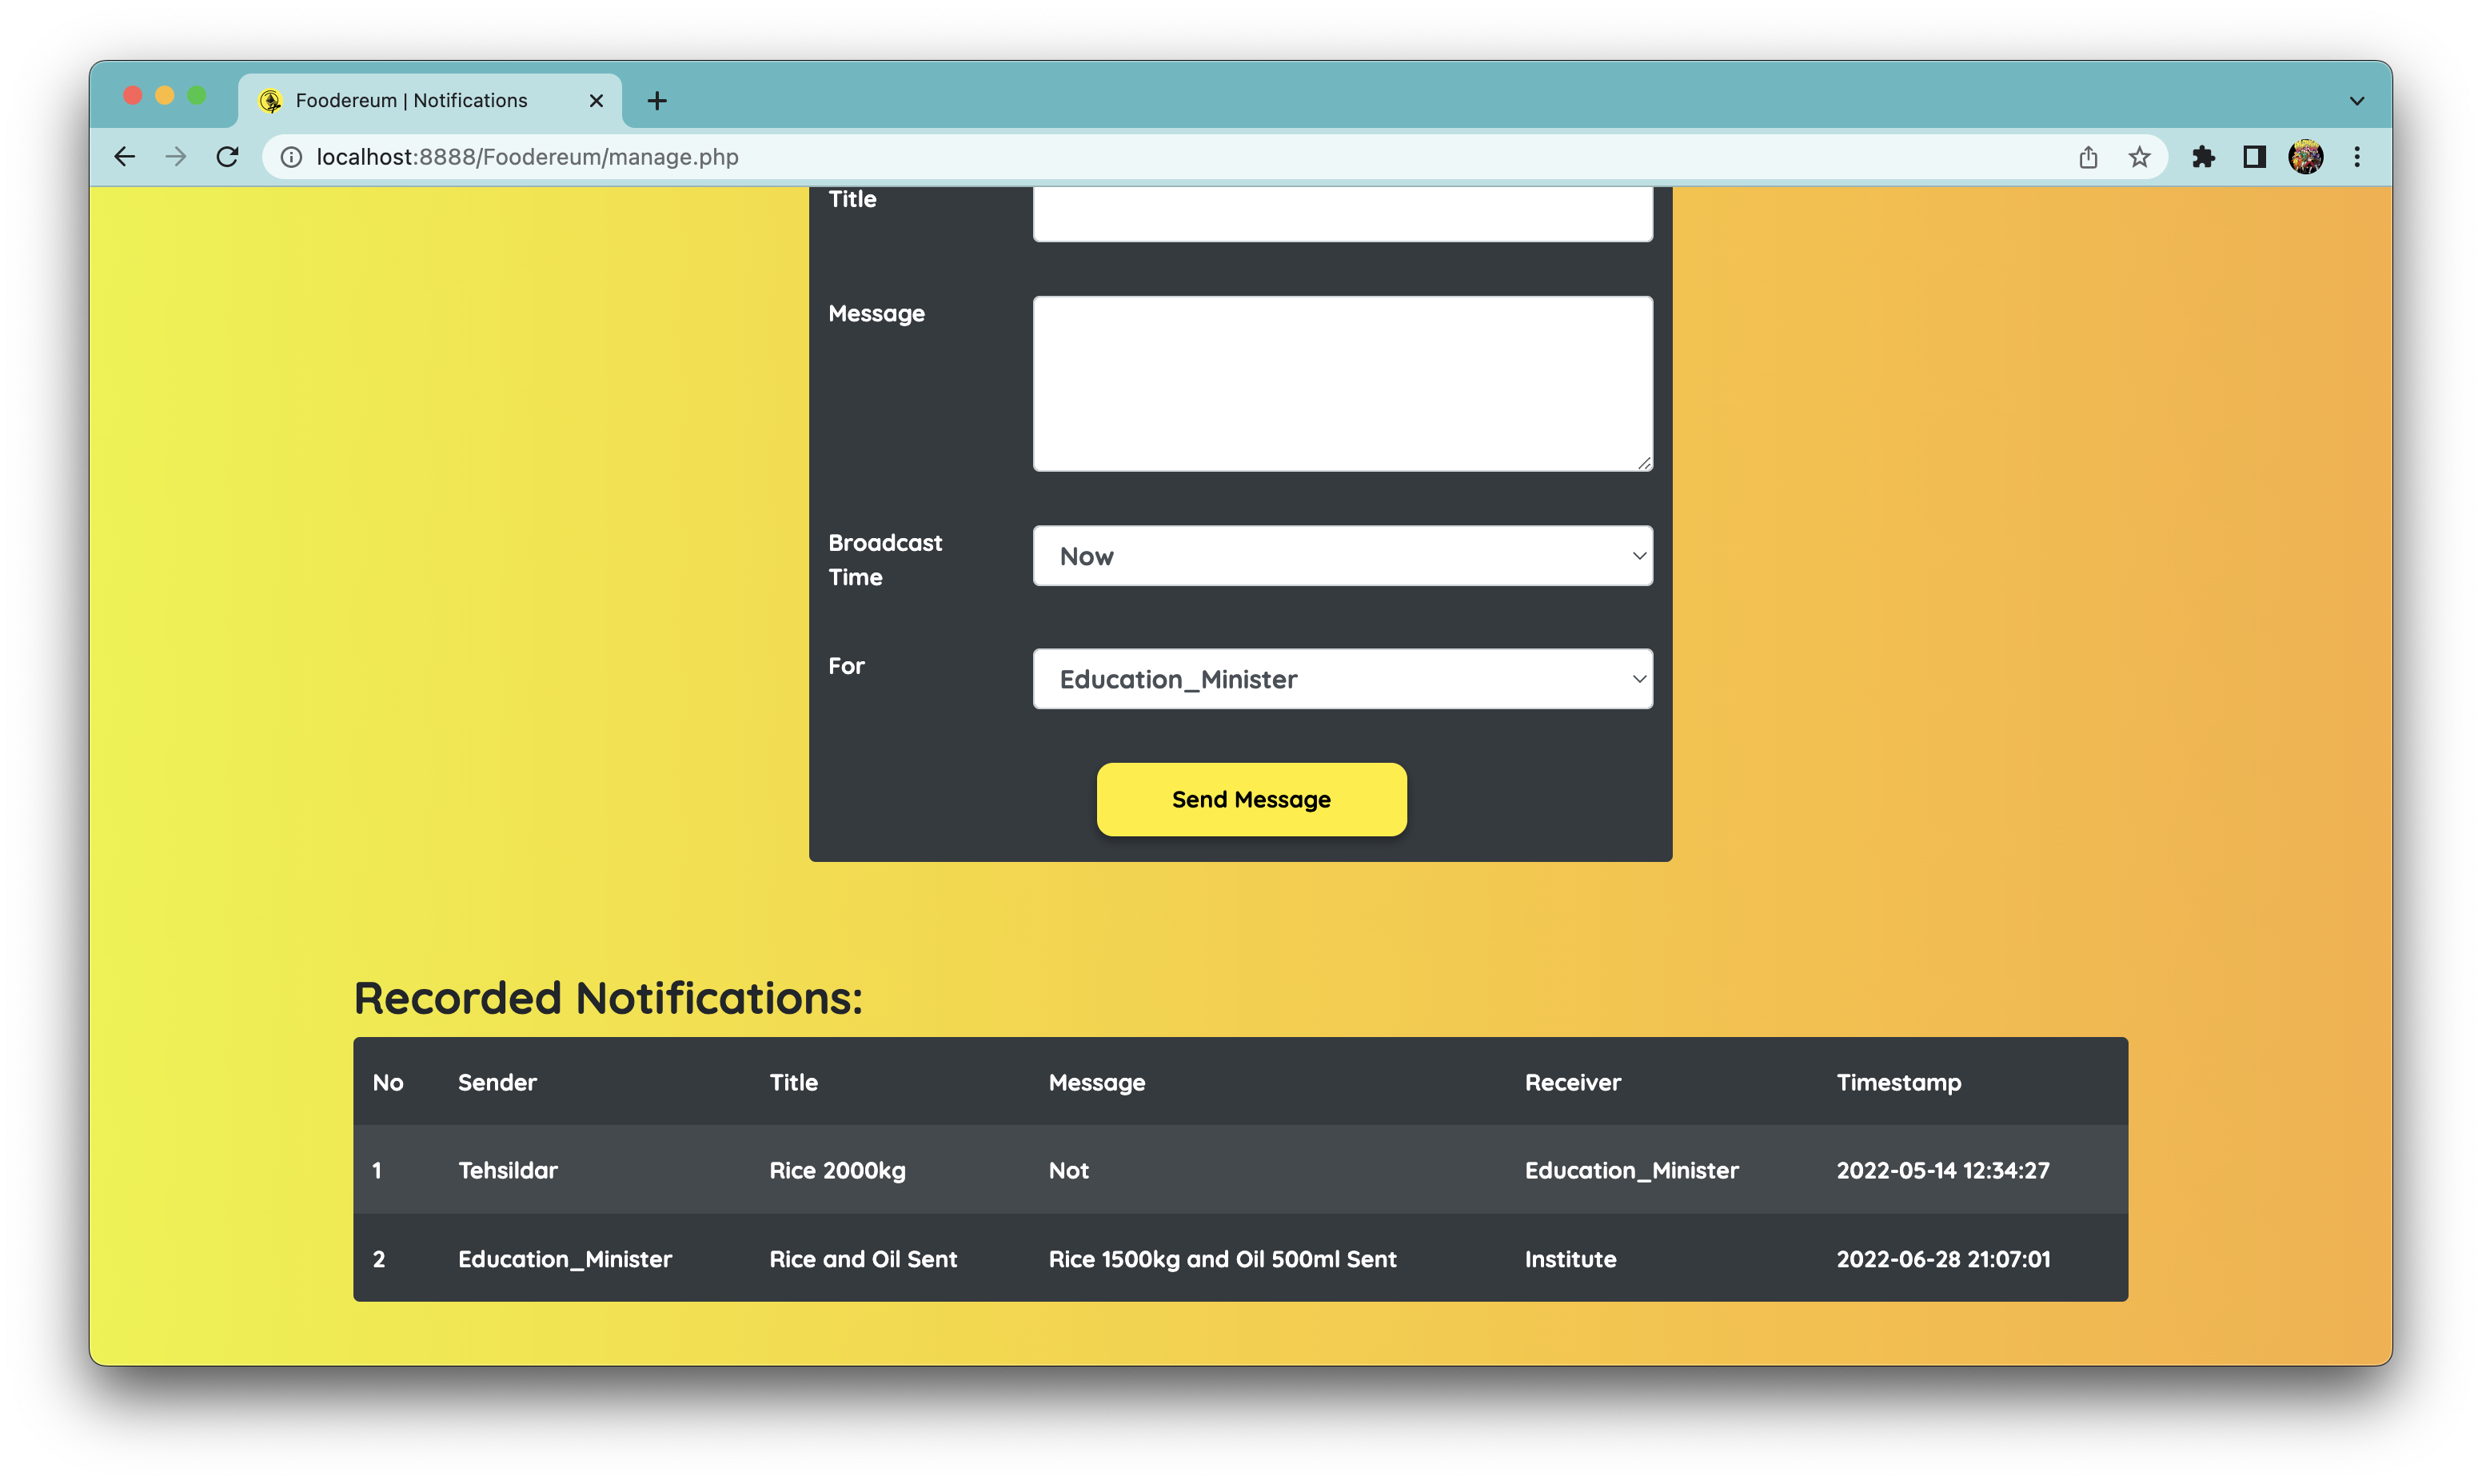
\includegraphics[width=15cm]{media/Notif_List.png}
\centering
\caption{List of Notifications}
\end{figure}
\begin{figure} [H]
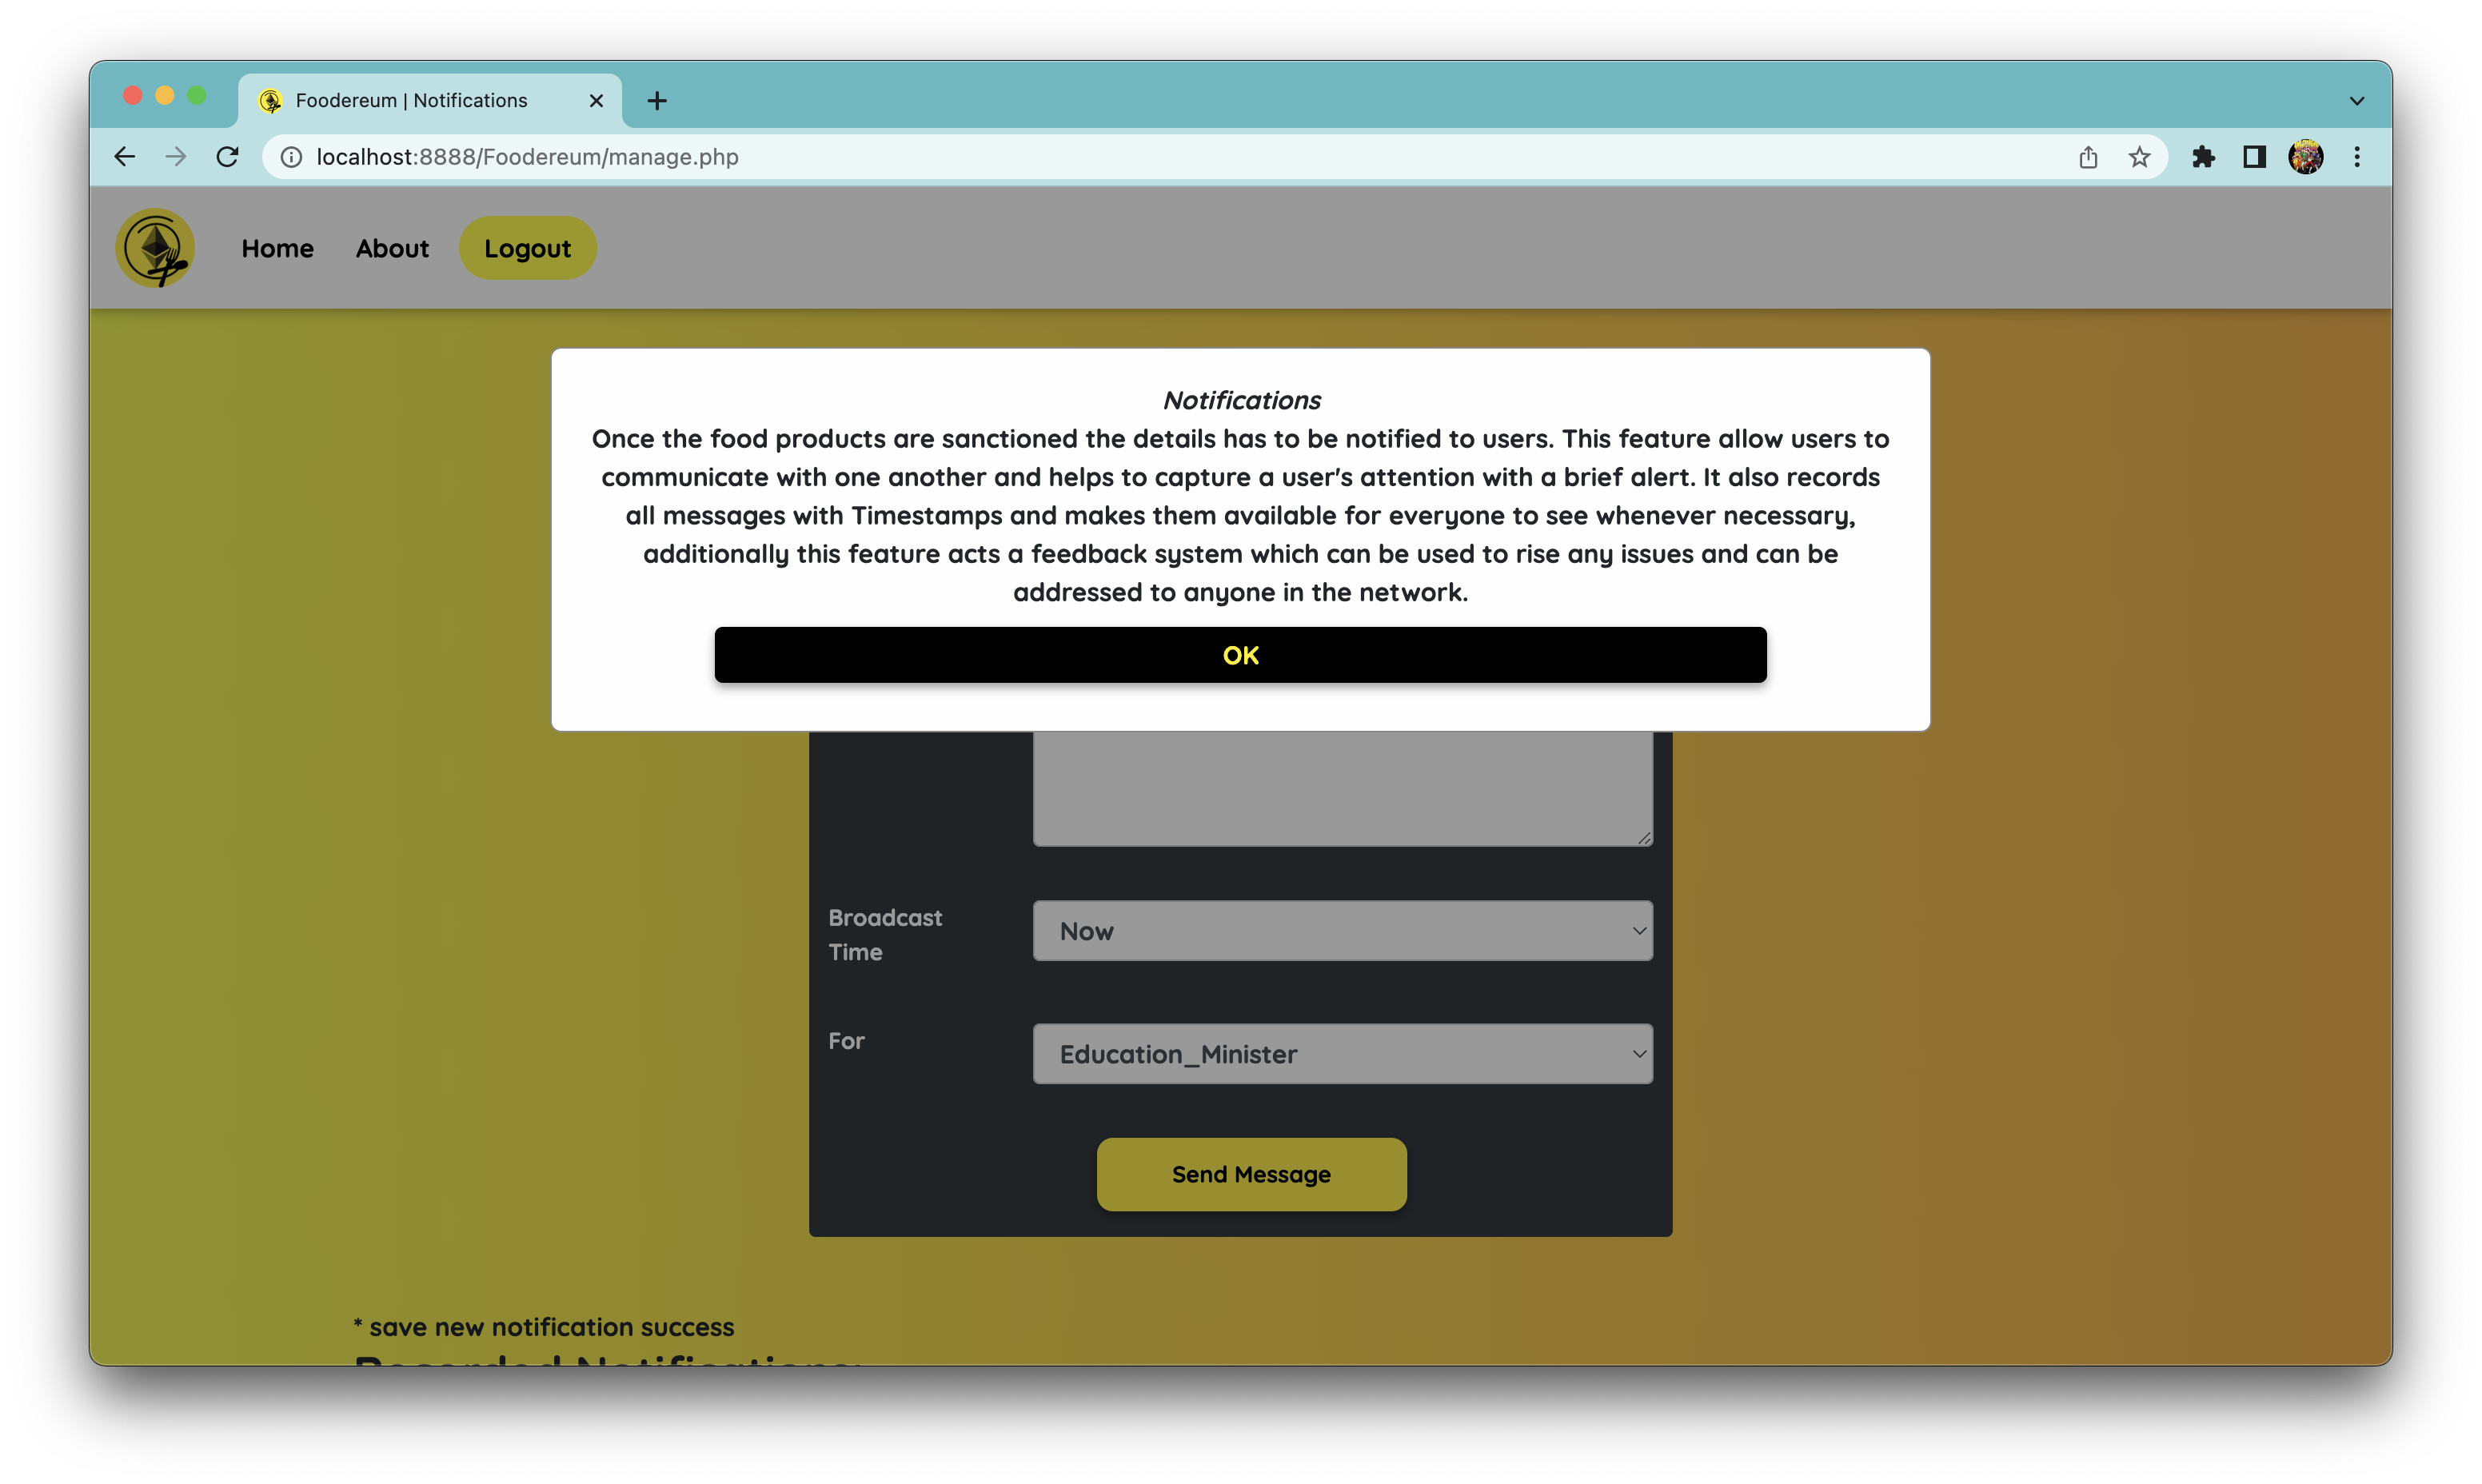
\includegraphics[width=15cm]{media/Notif_About.png}
\centering
\caption{Notifications About Page}
\end{figure}
\subsection{Analysis of Gas Consumption by Smart Contract \& its functions}
\begin{figure} [H]
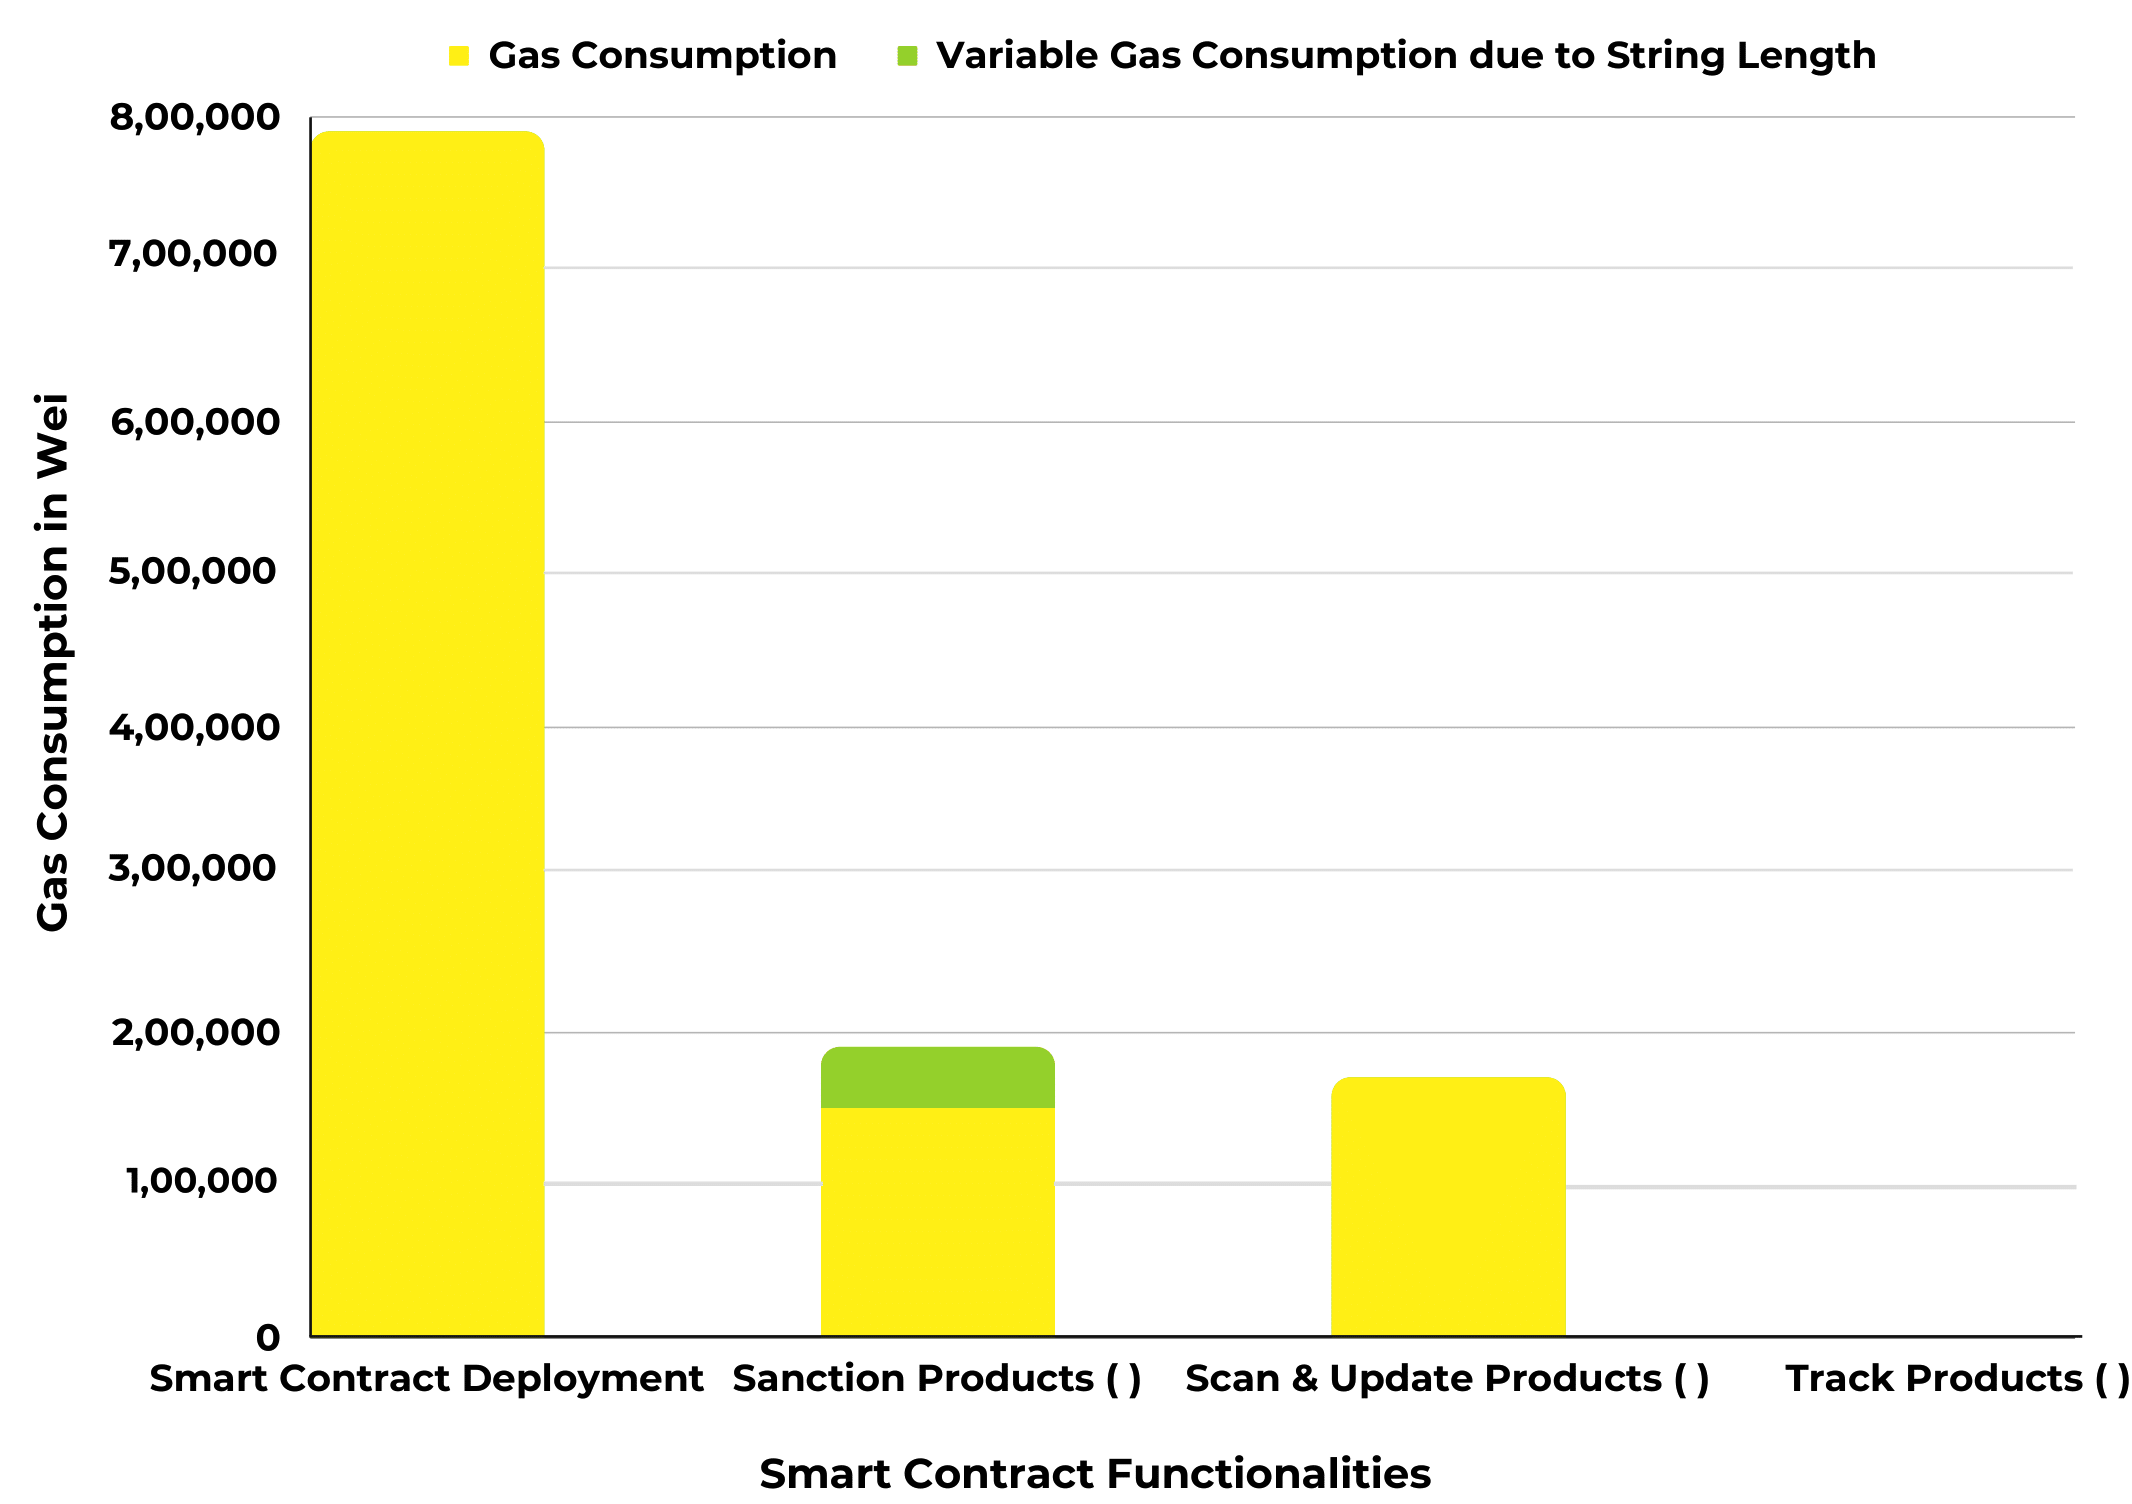
\includegraphics[width=15cm]{media/Gas.png}
\centering
\caption{Gas consumption vs Smart contract and its functions}
\end{figure}
Figure 6.14 depicts a detailed analysis of gas consumption in terms of Wei of the smart contract and its functions. It is clearly evident that deploying the smart contract in the Ethereum Blockchain takes the maximum value in terms of Wei, compared to any other smart contract functions. Our project Foodereum consists of three different smart contract functions, which are: Sanction Products ( ), Scan \& Update Products ( ) and Track Products ( ). 

The Sanction products( ) accepts the Product name and its quantity as inputs in strings, and spends highest gas value compared to the other two smart contract functions, as this function is accounted for registering the food commodities which are sanctioned by the sanctioner in the chain,  and then the products are recorded against the sanctioner’s profile in blockchain. It is observed that, as the input string length increases, the amount of gas spent by the function also increases, thus there is a slight variation in gas consumption with respect to the string length. 

The Scan \& Update products ( ) spends relatively less gas compared to Sanction Products ( ), as this function is used while shipping the products at different regions, for which it contains the details of the products which are sanctioned earlier. There is no considerable variability involved in gas consumption when the function is triggered.

The Track product ( ) is the only functionality that is offered to all the entities in the supply chain, this feature tends to spend no gas in the system. As tracking plays a crucial role in a supply chain environment, and its usage can be very frequent, due to which, to view the details of sanctioned products which are record on blockchain made reliable. This feature ensures complete traceability and transparency in the supply chain.
\newpage
  \pagestyle{fancy}
  \thispagestyle{empty}
  \thispagestyle{plain}
  \fancyhf{}
  \lhead{Foodereum: A Blockchain-based Authenticated Solution for Food Supply Chain $|$}
  \chead{}
  \rhead{Batch No.: 41}
  \renewcommand{\headrulewidth}{0.4pt}%
  \rfoot{Page \thepage \hspace{1pt} of \pageref{LastPage}}
  \lfoot{Dept. of CSE, DSCE}
\renewcommand{\footrulewidth}{0.4pt}%
\normalsize
\section*{Conclusion} 

The conventional Food Supply Chain spanning different nations provides customers with access to fresh and nutritious food. The food industry plays a vital role in supplying the essentials and needs for numerous human activities. However, the present supply chain merely monitor and store orders and shipments without incorporating crucial features such as transparency, traceability, and auditability. A lack of transparency and traceability as a result of centralised systems, third-party involvement during shipment, expensive transportation and storage costs, food waste due to rotting and contamination, insufficient accountability of organisations involved, and communication gaps between supply chain partners highlight the system's inefficiencies. By overcoming these hurdles, food quality and safety will increase, gaining appeal among consumers. \\

In order to help organisations record, track, and verify food goods along the supply chain, we propose an Ethereum-based authentication system for food programmes. Since the blockchain's immutability is one of its benefits, transactions cannot be altered or concealed since they are all recorded in a distributed ledger that can be tracked and made public to everyone with access to the data. This suggests that whenever a product is delivered, a new receiver will have access to the product's whole history on the blockchain network. \\
\subsection*{Future Enhancements:}
\begin{itemize}
    \item Enhancing food product traceability and accountability through the use of Internet of Things-based sensors, cameras, RFIDs, etc.
    \item Supporting distribution across several areas would increase the scalability of the current system.
    \item Simplifying the Decentralized app login process by connecting the platform to a Metamask account. It also provides good security.
\end{itemize}
\newpage
  \pagestyle{fancy}
  \fancyhf{}
  \lhead{Foodereum: A Blockchain-based Authenticated Solution for Food Supply Chain $|$}
  \chead{}
  \rhead{Batch No.: 41}
  \rfoot{Page \thepage \hspace{1pt} of \pageref{LastPage}}
  \lfoot{Dept. of CSE, DSCE}
\renewcommand{\footrulewidth}{0.4pt}% 
\normalsize
\LARGE{\textbf{References}} 
\normalsize
\let\lbrack[
\let\rbrack]
\begin{enumerate}[\lbrack1{\rbrack}]
    \item C. Verdouw, H. Sundmaeker, F. Meyer, J. Wolfert, and J. Verhoosel, “Smart agri-food logistics: requirements for the future internet,” in Dynamics in Logistics. Springer, 2013, pp. 247–257.
    \item M. Fartitchou, K. E. Makkaoui, N. Kannouf and Z. E. Allali, "Security on Blockchain Technology," 2020 3rd International Conference on Advanced Communication Technologies and Networking (CommNet), 2020, pp. 1-7, doi: 10.1109/CommNet49926.2020.9199622.
    \item B. Singhal, G. Dhameja, P. S. Panda, “Beginning Blockchain: A Beginner’s Guide to Building Blockchain Solutions,” Apress, 2018.
    \item D. Mazzei, et al., “A Blockchain Tokenizer for Industrial IOT trustless applications,” Future Generation Computer Systems, vol. 105, pp. 432– 445, 2020.
    \item H. Lee, M. Ma, “Blockchain-based mobility management for 5G,” Future Generation Computer Systems, 2019.
    \item Johar, S.; Ahmad, N.; Asher, W.; Cruickshank, H.; Durrani, A. Research and Applied Perspective to Blockchain Technology: A Comprehensive Survey. Appl. Sci. 2021, 11, 6252. 
    \item M. P. Caro, M. S. Ali, M. Vecchio and R. Giaffreda, "Blockchain-based traceability in Agri-Food supply chain management: A practical implementation," 2018 IoT Vertical and Topical Summit on Agriculture - Tuscany (IOT Tuscany), 2018, pp. 1-4, doi: 10.1109/IOT-TUSCANY.2018.8373021.
    \item B. Thuraisingham, "Blockchain Technologies and Their Applications in Data Science and Cyber Security," 2020 3rd International Conference on Smart BlockChain (SmartBlock), 2020, pp. 1-4, doi: 10.1109/SmartBlock52591.2020.00008.
    \item  Affaf Shahid, Umair Sarfraz, Muhammad Waseem Malik, Muhammad SohaibIftikhar, Abid Jamal, and Nadeem Javaid (2020). Blockchain-based Reputation System in Agri-Food Supply Chain. 
    \item Shivendra, K. Chiranjeevi, M. K. Tripathi and D. D. Maktedar, "Block chain Technology in Agriculture Product Supply Chain," 2021 International Conference on Artificial Intelligence and Smart Systems (ICAIS), 2021, pp. 1325-1329, doi: 10.1109/ICAIS50930.2021.9395886.
\end{enumerate}
\newpage
  \pagestyle{fancy}
  \fancyhf{}
  \lhead{Foodereum: A Blockchain-based Authenticated Solution for Food Supply Chain $|$}
  \chead{}
  \rhead{Batch No.: 41}
  \rfoot{Page \thepage \hspace{1pt} of \pageref{LastPage}}
  \lfoot{Dept. of CSE, DSCE}
\renewcommand{\footrulewidth}{0.4pt}% 
\normalsize
\section{Appendix} 
\subsection*{Solidity Smart Contract Code:} 
\definecolor{dkgreen}{rgb}{0,0.6,0}
\definecolor{gray}{rgb}{0.5,0.5,0.5}
\definecolor{mauve}{rgb}{0.58,0,0.82}

\lstset{frame=tb,
  language=Java,
  aboveskip=3mm,
  belowskip=3mm,
  showstringspaces=false,
  columns=flexible,
  basicstyle={\small\ttfamily},
  numbers=none,
  numberstyle=\tiny\color{gray},
  keywordstyle=\color{blue},
  commentstyle=\color{dkgreen},
  stringstyle=\color{mauve},
  breaklines=true,
  breakatwhitespace=true,
  tabsize=3
}
\begin{lstlisting}
// Foodereum.sol
pragma solidity ^0.6.0;

contract Foodereum {
    event Added(uint256 index);
    
    struct State {
        string details;
        address user;
    }
    
    struct FoodProduct {
        address creator;
        string productName;
        uint256 productId;
        string date;
        uint256 totalStates;
        mapping (uint256 => State) positions;
    }
    
    mapping(uint => FoodProduct) allProducts;
    uint256 items=0;
    
    function concat(string memory a,string memory b) public pure returns (string memory) {
        return string(abi.encodePacked(a,'',b));
    }
    
    
    
    
    function sanction(string memory _text, string memory _date) public returns (bool) {
        FoodProduct memory sanction = FoodProduct({creator: msg.sender, totalStates: 0,productName: _text, productId: items, date: _date});
        allProducts[items]=sanction;
        items = items+1;
        emit Added(items-1);
        return true;
    }
    
    function update(uint _productId, string memory info) public returns (string memory) {
        require(_productId<=items);
        State memory newState = State({user: msg.sender, details: info});
        allProducts[_productId].positions[ allProducts[_productId].totalStates ]=newState;
        allProducts[_productId].totalStates = allProducts[_productId].totalStates +1;
        return info;
    }
    
    function trackProduct(uint _productId) public returns (string memory) {
        require(_productId<=items);
        string memory output="<b>Product Name: </b>";
        output=concat(output, allProducts[_productId].productName);
        output=concat(output, "<br><b>Sanctioned Date: </b>");
        output=concat(output, allProducts[_productId].date);
       
        for (uint256 j=0; j<allProducts[_productId].totalStates; j++){
            output=concat(output, allProducts[_productId].positions[j].details);
        }
        return output;
    }
}
\end{lstlisting}
\end{document}


